\documentclass[twoside]{book}

% Packages required by doxygen
\usepackage{fixltx2e}
\usepackage{calc}
\usepackage{doxygen}
\usepackage[export]{adjustbox} % also loads graphicx
\usepackage{graphicx}
\usepackage[utf8]{inputenc}
\usepackage{makeidx}
\usepackage{multicol}
\usepackage{multirow}
\PassOptionsToPackage{warn}{textcomp}
\usepackage{textcomp}
\usepackage[nointegrals]{wasysym}
\usepackage[table]{xcolor}

% Font selection
\usepackage[T1]{fontenc}
\usepackage[scaled=.90]{helvet}
\usepackage{courier}
\usepackage{amssymb}
\usepackage{sectsty}
\renewcommand{\familydefault}{\sfdefault}
\allsectionsfont{%
  \fontseries{bc}\selectfont%
  \color{darkgray}%
}
\renewcommand{\DoxyLabelFont}{%
  \fontseries{bc}\selectfont%
  \color{darkgray}%
}
\newcommand{\+}{\discretionary{\mbox{\scriptsize$\hookleftarrow$}}{}{}}

% Page & text layout
\usepackage{geometry}
\geometry{%
  a4paper,%
  top=2.5cm,%
  bottom=2.5cm,%
  left=2.5cm,%
  right=2.5cm%
}
\tolerance=750
\hfuzz=15pt
\hbadness=750
\setlength{\emergencystretch}{15pt}
\setlength{\parindent}{0cm}
\setlength{\parskip}{3ex plus 2ex minus 2ex}
\makeatletter
\renewcommand{\paragraph}{%
  \@startsection{paragraph}{4}{0ex}{-1.0ex}{1.0ex}{%
    \normalfont\normalsize\bfseries\SS@parafont%
  }%
}
\renewcommand{\subparagraph}{%
  \@startsection{subparagraph}{5}{0ex}{-1.0ex}{1.0ex}{%
    \normalfont\normalsize\bfseries\SS@subparafont%
  }%
}
\makeatother

% Headers & footers
\usepackage{fancyhdr}
\pagestyle{fancyplain}
\fancyhead[LE]{\fancyplain{}{\bfseries\thepage}}
\fancyhead[CE]{\fancyplain{}{}}
\fancyhead[RE]{\fancyplain{}{\bfseries\leftmark}}
\fancyhead[LO]{\fancyplain{}{\bfseries\rightmark}}
\fancyhead[CO]{\fancyplain{}{}}
\fancyhead[RO]{\fancyplain{}{\bfseries\thepage}}
\fancyfoot[LE]{\fancyplain{}{}}
\fancyfoot[CE]{\fancyplain{}{}}
\fancyfoot[RE]{\fancyplain{}{\bfseries\scriptsize Generated by Doxygen }}
\fancyfoot[LO]{\fancyplain{}{\bfseries\scriptsize Generated by Doxygen }}
\fancyfoot[CO]{\fancyplain{}{}}
\fancyfoot[RO]{\fancyplain{}{}}
\renewcommand{\footrulewidth}{0.4pt}
\renewcommand{\chaptermark}[1]{%
  \markboth{#1}{}%
}
\renewcommand{\sectionmark}[1]{%
  \markright{\thesection\ #1}%
}

% Indices & bibliography
\usepackage{natbib}
\usepackage[titles]{tocloft}
\setcounter{tocdepth}{3}
\setcounter{secnumdepth}{5}
\makeindex

% Hyperlinks (required, but should be loaded last)
\usepackage{ifpdf}
\ifpdf
  \usepackage[pdftex,pagebackref=true]{hyperref}
\else
  \usepackage[ps2pdf,pagebackref=true]{hyperref}
\fi
\hypersetup{%
  colorlinks=true,%
  linkcolor=blue,%
  citecolor=blue,%
  unicode%
}

% Custom commands
\newcommand{\clearemptydoublepage}{%
  \newpage{\pagestyle{empty}\cleardoublepage}%
}

\usepackage{caption}
\captionsetup{labelsep=space,justification=centering,font={bf},singlelinecheck=off,skip=4pt,position=top}

%===== C O N T E N T S =====

\begin{document}

% Titlepage & ToC
\hypersetup{pageanchor=false,
             bookmarksnumbered=true,
             pdfencoding=unicode
            }
\pagenumbering{alph}
\begin{titlepage}
\vspace*{7cm}
\begin{center}%
{\Large Faded \\[1ex]\large 0.\+0.\+1 }\\
\vspace*{1cm}
{\large Generated by Doxygen 1.8.13}\\
\end{center}
\end{titlepage}
\clearemptydoublepage
\pagenumbering{roman}
\tableofcontents
\clearemptydoublepage
\pagenumbering{arabic}
\hypersetup{pageanchor=true}

%--- Begin generated contents ---
\chapter{Data Structure Index}
\section{Data Structures}
Here are the data structures with brief descriptions\+:\begin{DoxyCompactList}
\item\contentsline{section}{\hyperlink{structChrono}{Chrono} }{\pageref{structChrono}}{}
\item\contentsline{section}{\hyperlink{structEnnemy}{Ennemy} }{\pageref{structEnnemy}}{}
\item\contentsline{section}{\hyperlink{structgame}{game} }{\pageref{structgame}}{}
\item\contentsline{section}{\hyperlink{structoptions}{options} }{\pageref{structoptions}}{}
\item\contentsline{section}{\hyperlink{structPlayer}{Player} }{\pageref{structPlayer}}{}
\item\contentsline{section}{\hyperlink{structScroll}{Scroll} }{\pageref{structScroll}}{}
\item\contentsline{section}{\hyperlink{structtexte}{texte} }{\pageref{structtexte}}{}
\item\contentsline{section}{\hyperlink{structVie}{Vie} }{\pageref{structVie}}{}
\end{DoxyCompactList}

\chapter{File Index}
\section{File List}
Here is a list of all files with brief descriptions\+:\begin{DoxyCompactList}
\item\contentsline{section}{\hyperlink{bounding_8c}{bounding.\+c} }{\pageref{bounding_8c}}{}
\item\contentsline{section}{\hyperlink{bounding_8h}{bounding.\+h} }{\pageref{bounding_8h}}{}
\item\contentsline{section}{\hyperlink{chrono_8c}{chrono.\+c} }{\pageref{chrono_8c}}{}
\item\contentsline{section}{\hyperlink{chrono_8h}{chrono.\+h} }{\pageref{chrono_8h}}{}
\item\contentsline{section}{\hyperlink{chronometre_8c}{chronometre.\+c} }{\pageref{chronometre_8c}}{}
\item\contentsline{section}{\hyperlink{collisionparfait_8c}{collisionparfait.\+c} }{\pageref{collisionparfait_8c}}{}
\item\contentsline{section}{\hyperlink{collisionparfait_8h}{collisionparfait.\+h} }{\pageref{collisionparfait_8h}}{}
\item\contentsline{section}{\hyperlink{enigme1_8c}{enigme1.\+c} }{\pageref{enigme1_8c}}{}
\item\contentsline{section}{\hyperlink{enigmes_8c}{enigmes.\+c} \\*Toutes les enigmes }{\pageref{enigmes_8c}}{}
\item\contentsline{section}{\hyperlink{enigmes_8h}{enigmes.\+h} \\*Toutes les enigmes }{\pageref{enigmes_8h}}{}
\item\contentsline{section}{\hyperlink{ennemy_8c}{ennemy.\+c} }{\pageref{ennemy_8c}}{}
\item\contentsline{section}{\hyperlink{ennemy_8h}{ennemy.\+h} }{\pageref{ennemy_8h}}{}
\item\contentsline{section}{\hyperlink{fonctions_8c}{fonctions.\+c} \\*All the menu functions }{\pageref{fonctions_8c}}{}
\item\contentsline{section}{\hyperlink{fonctions_8h}{fonctions.\+h} \\*All the menu functions }{\pageref{fonctions_8h}}{}
\item\contentsline{section}{\hyperlink{game_8c}{game.\+c} }{\pageref{game_8c}}{}
\item\contentsline{section}{\hyperlink{game_8h}{game.\+h} }{\pageref{game_8h}}{}
\item\contentsline{section}{\hyperlink{levels_8c}{levels.\+c} }{\pageref{levels_8c}}{}
\item\contentsline{section}{\hyperlink{menu1_8c}{menu1.\+c} }{\pageref{menu1_8c}}{}
\item\contentsline{section}{\hyperlink{player_8c}{player.\+c} }{\pageref{player_8c}}{}
\item\contentsline{section}{\hyperlink{player_8h}{player.\+h} }{\pageref{player_8h}}{}
\item\contentsline{section}{\hyperlink{scrol_8c}{scrol.\+c} }{\pageref{scrol_8c}}{}
\item\contentsline{section}{\hyperlink{scrol_8h}{scrol.\+h} }{\pageref{scrol_8h}}{}
\item\contentsline{section}{\hyperlink{testmenu_8c}{testmenu.\+c} }{\pageref{testmenu_8c}}{}
\item\contentsline{section}{\hyperlink{vie_8c}{vie.\+c} }{\pageref{vie_8c}}{}
\item\contentsline{section}{\hyperlink{vie_8h}{vie.\+h} }{\pageref{vie_8h}}{}
\end{DoxyCompactList}

\chapter{Data Structure Documentation}
\hypertarget{structChrono}{}\section{Chrono Struct Reference}
\label{structChrono}\index{Chrono@{Chrono}}


{\ttfamily \#include $<$chrono.\+h$>$}

\subsection*{Data Fields}
\begin{DoxyCompactItemize}
\item 
Uint32 \hyperlink{structChrono_a3061de9a7108e54394d1d0e24a0ffc44}{current\+Time}
\item 
Uint32 \hyperlink{structChrono_a5f7678a92f46de2036caacb5b6f1e0a4}{last\+Time}
\item 
int \hyperlink{structChrono_ac3290e54ec8f6209808638edfee599fb}{counter}
\item 
bool \hyperlink{structChrono_a27a67b8bc1f8f46ad870a40aca82894d}{pause}
\item 
S\+D\+L\+\_\+\+Surface $\ast$ \hyperlink{structChrono_aa9e2794c88d9bc44f89aca45c4d7c55a}{texte}
\item 
S\+D\+L\+\_\+\+Rect \hyperlink{structChrono_a87a2242ec61dc7371f4a499a496edb42}{position}
\item 
T\+T\+F\+\_\+\+Font $\ast$ \hyperlink{structChrono_a57542d11a99ebc2675c72b0161ac5ab6}{police}
\item 
S\+D\+L\+\_\+\+Color \hyperlink{structChrono_a4d1eaa788972d858bcc6288b07768b5a}{couleur}
\end{DoxyCompactItemize}


\subsection{Field Documentation}
\mbox{\Hypertarget{structChrono_a4d1eaa788972d858bcc6288b07768b5a}\label{structChrono_a4d1eaa788972d858bcc6288b07768b5a}} 
\index{Chrono@{Chrono}!couleur@{couleur}}
\index{couleur@{couleur}!Chrono@{Chrono}}
\subsubsection{\texorpdfstring{couleur}{couleur}}
{\footnotesize\ttfamily S\+D\+L\+\_\+\+Color Chrono\+::couleur}

\mbox{\Hypertarget{structChrono_ac3290e54ec8f6209808638edfee599fb}\label{structChrono_ac3290e54ec8f6209808638edfee599fb}} 
\index{Chrono@{Chrono}!counter@{counter}}
\index{counter@{counter}!Chrono@{Chrono}}
\subsubsection{\texorpdfstring{counter}{counter}}
{\footnotesize\ttfamily int Chrono\+::counter}

\mbox{\Hypertarget{structChrono_a3061de9a7108e54394d1d0e24a0ffc44}\label{structChrono_a3061de9a7108e54394d1d0e24a0ffc44}} 
\index{Chrono@{Chrono}!current\+Time@{current\+Time}}
\index{current\+Time@{current\+Time}!Chrono@{Chrono}}
\subsubsection{\texorpdfstring{current\+Time}{currentTime}}
{\footnotesize\ttfamily Uint32 Chrono\+::current\+Time}

\mbox{\Hypertarget{structChrono_a5f7678a92f46de2036caacb5b6f1e0a4}\label{structChrono_a5f7678a92f46de2036caacb5b6f1e0a4}} 
\index{Chrono@{Chrono}!last\+Time@{last\+Time}}
\index{last\+Time@{last\+Time}!Chrono@{Chrono}}
\subsubsection{\texorpdfstring{last\+Time}{lastTime}}
{\footnotesize\ttfamily Uint32 Chrono\+::last\+Time}

\mbox{\Hypertarget{structChrono_a27a67b8bc1f8f46ad870a40aca82894d}\label{structChrono_a27a67b8bc1f8f46ad870a40aca82894d}} 
\index{Chrono@{Chrono}!pause@{pause}}
\index{pause@{pause}!Chrono@{Chrono}}
\subsubsection{\texorpdfstring{pause}{pause}}
{\footnotesize\ttfamily bool Chrono\+::pause}

\mbox{\Hypertarget{structChrono_a57542d11a99ebc2675c72b0161ac5ab6}\label{structChrono_a57542d11a99ebc2675c72b0161ac5ab6}} 
\index{Chrono@{Chrono}!police@{police}}
\index{police@{police}!Chrono@{Chrono}}
\subsubsection{\texorpdfstring{police}{police}}
{\footnotesize\ttfamily T\+T\+F\+\_\+\+Font$\ast$ Chrono\+::police}

\mbox{\Hypertarget{structChrono_a87a2242ec61dc7371f4a499a496edb42}\label{structChrono_a87a2242ec61dc7371f4a499a496edb42}} 
\index{Chrono@{Chrono}!position@{position}}
\index{position@{position}!Chrono@{Chrono}}
\subsubsection{\texorpdfstring{position}{position}}
{\footnotesize\ttfamily S\+D\+L\+\_\+\+Rect Chrono\+::position}

\mbox{\Hypertarget{structChrono_aa9e2794c88d9bc44f89aca45c4d7c55a}\label{structChrono_aa9e2794c88d9bc44f89aca45c4d7c55a}} 
\index{Chrono@{Chrono}!texte@{texte}}
\index{texte@{texte}!Chrono@{Chrono}}
\subsubsection{\texorpdfstring{texte}{texte}}
{\footnotesize\ttfamily S\+D\+L\+\_\+\+Surface$\ast$ Chrono\+::texte}



The documentation for this struct was generated from the following file\+:\begin{DoxyCompactItemize}
\item 
\hyperlink{chrono_8h}{chrono.\+h}\end{DoxyCompactItemize}

\hypertarget{structEnnemy}{}\section{Ennemy Struct Reference}
\label{structEnnemy}\index{Ennemy@{Ennemy}}


{\ttfamily \#include $<$ennemy.\+h$>$}

\subsection*{Data Fields}
\begin{DoxyCompactItemize}
\item 
S\+D\+L\+\_\+\+Surface $\ast$ \hyperlink{structEnnemy_a8b4bb002eeade326a908f36f46763490}{Animation\+\_\+G} \mbox{[}4\mbox{]}
\item 
S\+D\+L\+\_\+\+Surface $\ast$ \hyperlink{structEnnemy_a922bd100d0198e663b521dbc7a5289f9}{Animation\+\_\+D} \mbox{[}4\mbox{]}
\item 
int \hyperlink{structEnnemy_a15e3dcbde7c86ebdba79e7936e92dfe1}{Animation}
\item 
S\+D\+L\+\_\+\+Rect \hyperlink{structEnnemy_a37ae489643736f036ddae15bc86d00d0}{Position}
\item 
bool \hyperlink{structEnnemy_ae145eac6d968735d00d6b0426b3f14f4}{Direction}
\end{DoxyCompactItemize}


\subsection{Field Documentation}
\mbox{\Hypertarget{structEnnemy_a15e3dcbde7c86ebdba79e7936e92dfe1}\label{structEnnemy_a15e3dcbde7c86ebdba79e7936e92dfe1}} 
\index{Ennemy@{Ennemy}!Animation@{Animation}}
\index{Animation@{Animation}!Ennemy@{Ennemy}}
\subsubsection{\texorpdfstring{Animation}{Animation}}
{\footnotesize\ttfamily int Ennemy\+::\+Animation}

\mbox{\Hypertarget{structEnnemy_a922bd100d0198e663b521dbc7a5289f9}\label{structEnnemy_a922bd100d0198e663b521dbc7a5289f9}} 
\index{Ennemy@{Ennemy}!Animation\+\_\+D@{Animation\+\_\+D}}
\index{Animation\+\_\+D@{Animation\+\_\+D}!Ennemy@{Ennemy}}
\subsubsection{\texorpdfstring{Animation\+\_\+D}{Animation\_D}}
{\footnotesize\ttfamily S\+D\+L\+\_\+\+Surface$\ast$ Ennemy\+::\+Animation\+\_\+D\mbox{[}4\mbox{]}}

\mbox{\Hypertarget{structEnnemy_a8b4bb002eeade326a908f36f46763490}\label{structEnnemy_a8b4bb002eeade326a908f36f46763490}} 
\index{Ennemy@{Ennemy}!Animation\+\_\+G@{Animation\+\_\+G}}
\index{Animation\+\_\+G@{Animation\+\_\+G}!Ennemy@{Ennemy}}
\subsubsection{\texorpdfstring{Animation\+\_\+G}{Animation\_G}}
{\footnotesize\ttfamily S\+D\+L\+\_\+\+Surface$\ast$ Ennemy\+::\+Animation\+\_\+G\mbox{[}4\mbox{]}}

\mbox{\Hypertarget{structEnnemy_ae145eac6d968735d00d6b0426b3f14f4}\label{structEnnemy_ae145eac6d968735d00d6b0426b3f14f4}} 
\index{Ennemy@{Ennemy}!Direction@{Direction}}
\index{Direction@{Direction}!Ennemy@{Ennemy}}
\subsubsection{\texorpdfstring{Direction}{Direction}}
{\footnotesize\ttfamily bool Ennemy\+::\+Direction}

\mbox{\Hypertarget{structEnnemy_a37ae489643736f036ddae15bc86d00d0}\label{structEnnemy_a37ae489643736f036ddae15bc86d00d0}} 
\index{Ennemy@{Ennemy}!Position@{Position}}
\index{Position@{Position}!Ennemy@{Ennemy}}
\subsubsection{\texorpdfstring{Position}{Position}}
{\footnotesize\ttfamily S\+D\+L\+\_\+\+Rect Ennemy\+::\+Position}



The documentation for this struct was generated from the following file\+:\begin{DoxyCompactItemize}
\item 
\hyperlink{ennemy_8h}{ennemy.\+h}\end{DoxyCompactItemize}

\hypertarget{structgame}{}\section{game Struct Reference}
\label{structgame}\index{game@{game}}


{\ttfamily \#include $<$game.\+h$>$}



Collaboration diagram for game\+:\nopagebreak
\begin{figure}[H]
\begin{center}
\leavevmode
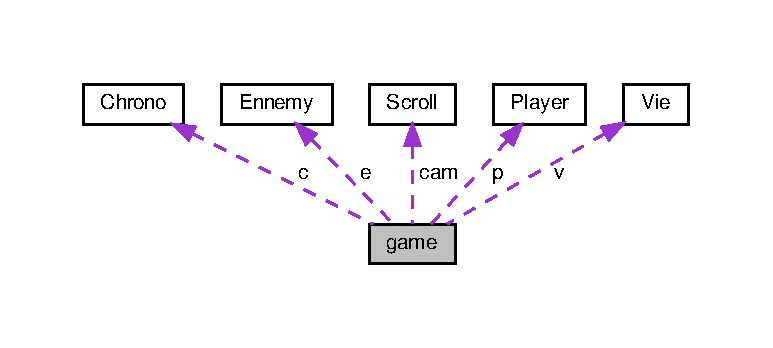
\includegraphics[width=350pt]{structgame__coll__graph}
\end{center}
\end{figure}
\subsection*{Data Fields}
\begin{DoxyCompactItemize}
\item 
\hyperlink{structEnnemy}{Ennemy} \hyperlink{structgame_a9a6f9c4dbbed53b3db30408494f16c86}{e}
\item 
\hyperlink{structVie}{Vie} \hyperlink{structgame_ace63f61e0876a3bcf5285db08b43cb36}{v}
\item 
\hyperlink{structPlayer}{Player} \hyperlink{structgame_a1089163f69974caccc1b3fd9cdb2618f}{p}
\item 
\hyperlink{structChrono}{Chrono} \hyperlink{structgame_acbb63e13f36a1a563e71f3c5585d535b}{c}
\item 
\hyperlink{structScroll}{Scroll} \hyperlink{structgame_a049a316142be533b4ac476db39e73b18}{cam}
\item 
bool \hyperlink{structgame_a2d4f5ae14a366168dd19da1e83cd8ad7}{Game\+Enigme}
\item 
int \hyperlink{structgame_ae06e10da51741dbe8cf2977512e81c94}{sc}
\item 
int \hyperlink{structgame_a6e10d564623857f7732c73dc10a8ec1d}{time}
\item 
S\+D\+L\+\_\+\+Rect \hyperlink{structgame_a4b5119efed4eee7a84685a7272921439}{pos\+\_\+real}
\item 
S\+D\+L\+\_\+\+Surface $\ast$ \hyperlink{structgame_ab299a67ca3fdaf9ca8c4b1dd5c99129b}{background}
\item 
S\+D\+L\+\_\+\+Surface $\ast$ \hyperlink{structgame_a16cce3e91de3f657879f73af44aa7a25}{backmask}
\item 
S\+D\+L\+\_\+\+Rect \hyperlink{structgame_aaf6e725d199a2b7e3b1ebecdf64b4614}{pos\+\_\+souris}
\item 
bool \hyperlink{structgame_a5a1947382819a3b6182741f70ec7916b}{Game\+Over}
\item 
bool \hyperlink{structgame_a054464e92ab87658ffa7935942e5c4ed}{collision}
\item 
int \hyperlink{structgame_a9c565166ec535e0abed46299c525a607}{col\+Parfait}
\item 
bool \hyperlink{structgame_ac0f89bfe27ab94ee9bdb23d028449b60}{kill}
\end{DoxyCompactItemize}


\subsection{Field Documentation}
\mbox{\Hypertarget{structgame_ab299a67ca3fdaf9ca8c4b1dd5c99129b}\label{structgame_ab299a67ca3fdaf9ca8c4b1dd5c99129b}} 
\index{game@{game}!background@{background}}
\index{background@{background}!game@{game}}
\subsubsection{\texorpdfstring{background}{background}}
{\footnotesize\ttfamily S\+D\+L\+\_\+\+Surface$\ast$ game\+::background}

\mbox{\Hypertarget{structgame_a16cce3e91de3f657879f73af44aa7a25}\label{structgame_a16cce3e91de3f657879f73af44aa7a25}} 
\index{game@{game}!backmask@{backmask}}
\index{backmask@{backmask}!game@{game}}
\subsubsection{\texorpdfstring{backmask}{backmask}}
{\footnotesize\ttfamily S\+D\+L\+\_\+\+Surface$\ast$ game\+::backmask}

\mbox{\Hypertarget{structgame_acbb63e13f36a1a563e71f3c5585d535b}\label{structgame_acbb63e13f36a1a563e71f3c5585d535b}} 
\index{game@{game}!c@{c}}
\index{c@{c}!game@{game}}
\subsubsection{\texorpdfstring{c}{c}}
{\footnotesize\ttfamily \hyperlink{structChrono}{Chrono} game\+::c}

\mbox{\Hypertarget{structgame_a049a316142be533b4ac476db39e73b18}\label{structgame_a049a316142be533b4ac476db39e73b18}} 
\index{game@{game}!cam@{cam}}
\index{cam@{cam}!game@{game}}
\subsubsection{\texorpdfstring{cam}{cam}}
{\footnotesize\ttfamily \hyperlink{structScroll}{Scroll} game\+::cam}

\mbox{\Hypertarget{structgame_a054464e92ab87658ffa7935942e5c4ed}\label{structgame_a054464e92ab87658ffa7935942e5c4ed}} 
\index{game@{game}!collision@{collision}}
\index{collision@{collision}!game@{game}}
\subsubsection{\texorpdfstring{collision}{collision}}
{\footnotesize\ttfamily bool game\+::collision}

\mbox{\Hypertarget{structgame_a9c565166ec535e0abed46299c525a607}\label{structgame_a9c565166ec535e0abed46299c525a607}} 
\index{game@{game}!col\+Parfait@{col\+Parfait}}
\index{col\+Parfait@{col\+Parfait}!game@{game}}
\subsubsection{\texorpdfstring{col\+Parfait}{colParfait}}
{\footnotesize\ttfamily int game\+::col\+Parfait}

\mbox{\Hypertarget{structgame_a9a6f9c4dbbed53b3db30408494f16c86}\label{structgame_a9a6f9c4dbbed53b3db30408494f16c86}} 
\index{game@{game}!e@{e}}
\index{e@{e}!game@{game}}
\subsubsection{\texorpdfstring{e}{e}}
{\footnotesize\ttfamily \hyperlink{structEnnemy}{Ennemy} game\+::e}

\mbox{\Hypertarget{structgame_a2d4f5ae14a366168dd19da1e83cd8ad7}\label{structgame_a2d4f5ae14a366168dd19da1e83cd8ad7}} 
\index{game@{game}!Game\+Enigme@{Game\+Enigme}}
\index{Game\+Enigme@{Game\+Enigme}!game@{game}}
\subsubsection{\texorpdfstring{Game\+Enigme}{GameEnigme}}
{\footnotesize\ttfamily bool game\+::\+Game\+Enigme}

\mbox{\Hypertarget{structgame_a5a1947382819a3b6182741f70ec7916b}\label{structgame_a5a1947382819a3b6182741f70ec7916b}} 
\index{game@{game}!Game\+Over@{Game\+Over}}
\index{Game\+Over@{Game\+Over}!game@{game}}
\subsubsection{\texorpdfstring{Game\+Over}{GameOver}}
{\footnotesize\ttfamily bool game\+::\+Game\+Over}

\mbox{\Hypertarget{structgame_ac0f89bfe27ab94ee9bdb23d028449b60}\label{structgame_ac0f89bfe27ab94ee9bdb23d028449b60}} 
\index{game@{game}!kill@{kill}}
\index{kill@{kill}!game@{game}}
\subsubsection{\texorpdfstring{kill}{kill}}
{\footnotesize\ttfamily bool game\+::kill}

\mbox{\Hypertarget{structgame_a1089163f69974caccc1b3fd9cdb2618f}\label{structgame_a1089163f69974caccc1b3fd9cdb2618f}} 
\index{game@{game}!p@{p}}
\index{p@{p}!game@{game}}
\subsubsection{\texorpdfstring{p}{p}}
{\footnotesize\ttfamily \hyperlink{structPlayer}{Player} game\+::p}

\mbox{\Hypertarget{structgame_a4b5119efed4eee7a84685a7272921439}\label{structgame_a4b5119efed4eee7a84685a7272921439}} 
\index{game@{game}!pos\+\_\+real@{pos\+\_\+real}}
\index{pos\+\_\+real@{pos\+\_\+real}!game@{game}}
\subsubsection{\texorpdfstring{pos\+\_\+real}{pos\_real}}
{\footnotesize\ttfamily S\+D\+L\+\_\+\+Rect game\+::pos\+\_\+real}

\mbox{\Hypertarget{structgame_aaf6e725d199a2b7e3b1ebecdf64b4614}\label{structgame_aaf6e725d199a2b7e3b1ebecdf64b4614}} 
\index{game@{game}!pos\+\_\+souris@{pos\+\_\+souris}}
\index{pos\+\_\+souris@{pos\+\_\+souris}!game@{game}}
\subsubsection{\texorpdfstring{pos\+\_\+souris}{pos\_souris}}
{\footnotesize\ttfamily S\+D\+L\+\_\+\+Rect game\+::pos\+\_\+souris}

\mbox{\Hypertarget{structgame_ae06e10da51741dbe8cf2977512e81c94}\label{structgame_ae06e10da51741dbe8cf2977512e81c94}} 
\index{game@{game}!sc@{sc}}
\index{sc@{sc}!game@{game}}
\subsubsection{\texorpdfstring{sc}{sc}}
{\footnotesize\ttfamily int game\+::sc}

\mbox{\Hypertarget{structgame_a6e10d564623857f7732c73dc10a8ec1d}\label{structgame_a6e10d564623857f7732c73dc10a8ec1d}} 
\index{game@{game}!time@{time}}
\index{time@{time}!game@{game}}
\subsubsection{\texorpdfstring{time}{time}}
{\footnotesize\ttfamily int game\+::time}

\mbox{\Hypertarget{structgame_ace63f61e0876a3bcf5285db08b43cb36}\label{structgame_ace63f61e0876a3bcf5285db08b43cb36}} 
\index{game@{game}!v@{v}}
\index{v@{v}!game@{game}}
\subsubsection{\texorpdfstring{v}{v}}
{\footnotesize\ttfamily \hyperlink{structVie}{Vie} game\+::v}



The documentation for this struct was generated from the following file\+:\begin{DoxyCompactItemize}
\item 
\hyperlink{game_8h}{game.\+h}\end{DoxyCompactItemize}

\hypertarget{structoptions}{}\section{options Struct Reference}
\label{structoptions}\index{options@{options}}


{\ttfamily \#include $<$fonctions.\+h$>$}

\subsection*{Data Fields}
\begin{DoxyCompactItemize}
\item 
S\+D\+L\+\_\+\+Surface $\ast$ \hyperlink{structoptions_a712af86841757c3f520dc5fe50edc5cb}{boutton}
\item 
S\+D\+L\+\_\+\+Rect \hyperlink{structoptions_af6da4211a6cb028c103f9471a374bb6e}{positionboutton}
\end{DoxyCompactItemize}


\subsection{Field Documentation}
\mbox{\Hypertarget{structoptions_a712af86841757c3f520dc5fe50edc5cb}\label{structoptions_a712af86841757c3f520dc5fe50edc5cb}} 
\index{options@{options}!boutton@{boutton}}
\index{boutton@{boutton}!options@{options}}
\subsubsection{\texorpdfstring{boutton}{boutton}}
{\footnotesize\ttfamily S\+D\+L\+\_\+\+Surface$\ast$ options\+::boutton}

\mbox{\Hypertarget{structoptions_af6da4211a6cb028c103f9471a374bb6e}\label{structoptions_af6da4211a6cb028c103f9471a374bb6e}} 
\index{options@{options}!positionboutton@{positionboutton}}
\index{positionboutton@{positionboutton}!options@{options}}
\subsubsection{\texorpdfstring{positionboutton}{positionboutton}}
{\footnotesize\ttfamily S\+D\+L\+\_\+\+Rect options\+::positionboutton}



The documentation for this struct was generated from the following file\+:\begin{DoxyCompactItemize}
\item 
\hyperlink{fonctions_8h}{fonctions.\+h}\end{DoxyCompactItemize}

\hypertarget{structPlayer}{}\section{Player Struct Reference}
\label{structPlayer}\index{Player@{Player}}


{\ttfamily \#include $<$player.\+h$>$}

\subsection*{Data Fields}
\begin{DoxyCompactItemize}
\item 
S\+D\+L\+\_\+\+Surface $\ast$ \hyperlink{structPlayer_a9dabac85ae31980a1b912694d89d95de}{DeplacementG} \mbox{[}6\mbox{]}
\item 
S\+D\+L\+\_\+\+Surface $\ast$ \hyperlink{structPlayer_acb3399f7e60d2be41d7aa1cee3ec4e66}{DeplacementD} \mbox{[}6\mbox{]}
\item 
S\+D\+L\+\_\+\+Surface $\ast$ \hyperlink{structPlayer_a6608c060fd0e9def58e13bad4f19d500}{AnimationG} \mbox{[}5\mbox{]}
\item 
S\+D\+L\+\_\+\+Surface $\ast$ \hyperlink{structPlayer_a5122ccb8f74095c280a24bfa19d390a7}{AnimationD} \mbox{[}5\mbox{]}
\item 
S\+D\+L\+\_\+\+Surface $\ast$ \hyperlink{structPlayer_a97acdb37024b80bb43aa293589ba2b22}{AttackG} \mbox{[}7\mbox{]}
\item 
S\+D\+L\+\_\+\+Surface $\ast$ \hyperlink{structPlayer_ae7482c585104ebbeb49fa60a8d6362f6}{AttackD} \mbox{[}7\mbox{]}
\item 
int \hyperlink{structPlayer_a3b144e1fee7b4f1baae1f26374416a85}{Animation}
\item 
S\+D\+L\+\_\+\+Rect \hyperlink{structPlayer_a790577b95757d4f7b27442264fdee116}{Position}
\item 
bool \hyperlink{structPlayer_ade89420a62ced088d3fd382af791cec3}{Direction}
\item 
bool \hyperlink{structPlayer_ac078c2779ae4431e571b6062d5e27c52}{Etat\+\_\+\+Mv}
\item 
bool \hyperlink{structPlayer_a38cd0b30353c30c150faa071198f5413}{Etat\+\_\+\+MvC}
\item 
int \hyperlink{structPlayer_adc1d5ec9edec35b7ed2a9eebc6d69d40}{Deplacement}
\item 
int \hyperlink{structPlayer_a0edea7ee3c5c7ef5d934fcafd9536c4f}{Ground}
\item 
int \hyperlink{structPlayer_a990b8343eb6aec2ce445f37b741c536f}{Jump}
\item 
int \hyperlink{structPlayer_a5282fb2b8a94ae294d5ed86a91a58d0d}{Attack}
\item 
int \hyperlink{structPlayer_af831c1c11251f76c63e99cc069517885}{attack}
\end{DoxyCompactItemize}


\subsection{Field Documentation}
\mbox{\Hypertarget{structPlayer_a3b144e1fee7b4f1baae1f26374416a85}\label{structPlayer_a3b144e1fee7b4f1baae1f26374416a85}} 
\index{Player@{Player}!Animation@{Animation}}
\index{Animation@{Animation}!Player@{Player}}
\subsubsection{\texorpdfstring{Animation}{Animation}}
{\footnotesize\ttfamily int Player\+::\+Animation}

\mbox{\Hypertarget{structPlayer_a5122ccb8f74095c280a24bfa19d390a7}\label{structPlayer_a5122ccb8f74095c280a24bfa19d390a7}} 
\index{Player@{Player}!AnimationD@{AnimationD}}
\index{AnimationD@{AnimationD}!Player@{Player}}
\subsubsection{\texorpdfstring{AnimationD}{AnimationD}}
{\footnotesize\ttfamily S\+D\+L\+\_\+\+Surface$\ast$ Player\+::\+AnimationD\mbox{[}5\mbox{]}}

\mbox{\Hypertarget{structPlayer_a6608c060fd0e9def58e13bad4f19d500}\label{structPlayer_a6608c060fd0e9def58e13bad4f19d500}} 
\index{Player@{Player}!AnimationG@{AnimationG}}
\index{AnimationG@{AnimationG}!Player@{Player}}
\subsubsection{\texorpdfstring{AnimationG}{AnimationG}}
{\footnotesize\ttfamily S\+D\+L\+\_\+\+Surface$\ast$ Player\+::\+AnimationG\mbox{[}5\mbox{]}}

\mbox{\Hypertarget{structPlayer_a5282fb2b8a94ae294d5ed86a91a58d0d}\label{structPlayer_a5282fb2b8a94ae294d5ed86a91a58d0d}} 
\index{Player@{Player}!Attack@{Attack}}
\index{Attack@{Attack}!Player@{Player}}
\subsubsection{\texorpdfstring{Attack}{Attack}}
{\footnotesize\ttfamily int Player\+::\+Attack}

\mbox{\Hypertarget{structPlayer_af831c1c11251f76c63e99cc069517885}\label{structPlayer_af831c1c11251f76c63e99cc069517885}} 
\index{Player@{Player}!attack@{attack}}
\index{attack@{attack}!Player@{Player}}
\subsubsection{\texorpdfstring{attack}{attack}}
{\footnotesize\ttfamily int Player\+::attack}

\mbox{\Hypertarget{structPlayer_ae7482c585104ebbeb49fa60a8d6362f6}\label{structPlayer_ae7482c585104ebbeb49fa60a8d6362f6}} 
\index{Player@{Player}!AttackD@{AttackD}}
\index{AttackD@{AttackD}!Player@{Player}}
\subsubsection{\texorpdfstring{AttackD}{AttackD}}
{\footnotesize\ttfamily S\+D\+L\+\_\+\+Surface$\ast$ Player\+::\+AttackD\mbox{[}7\mbox{]}}

\mbox{\Hypertarget{structPlayer_a97acdb37024b80bb43aa293589ba2b22}\label{structPlayer_a97acdb37024b80bb43aa293589ba2b22}} 
\index{Player@{Player}!AttackG@{AttackG}}
\index{AttackG@{AttackG}!Player@{Player}}
\subsubsection{\texorpdfstring{AttackG}{AttackG}}
{\footnotesize\ttfamily S\+D\+L\+\_\+\+Surface$\ast$ Player\+::\+AttackG\mbox{[}7\mbox{]}}

\mbox{\Hypertarget{structPlayer_adc1d5ec9edec35b7ed2a9eebc6d69d40}\label{structPlayer_adc1d5ec9edec35b7ed2a9eebc6d69d40}} 
\index{Player@{Player}!Deplacement@{Deplacement}}
\index{Deplacement@{Deplacement}!Player@{Player}}
\subsubsection{\texorpdfstring{Deplacement}{Deplacement}}
{\footnotesize\ttfamily int Player\+::\+Deplacement}

\mbox{\Hypertarget{structPlayer_acb3399f7e60d2be41d7aa1cee3ec4e66}\label{structPlayer_acb3399f7e60d2be41d7aa1cee3ec4e66}} 
\index{Player@{Player}!DeplacementD@{DeplacementD}}
\index{DeplacementD@{DeplacementD}!Player@{Player}}
\subsubsection{\texorpdfstring{DeplacementD}{DeplacementD}}
{\footnotesize\ttfamily S\+D\+L\+\_\+\+Surface$\ast$ Player\+::\+DeplacementD\mbox{[}6\mbox{]}}

\mbox{\Hypertarget{structPlayer_a9dabac85ae31980a1b912694d89d95de}\label{structPlayer_a9dabac85ae31980a1b912694d89d95de}} 
\index{Player@{Player}!DeplacementG@{DeplacementG}}
\index{DeplacementG@{DeplacementG}!Player@{Player}}
\subsubsection{\texorpdfstring{DeplacementG}{DeplacementG}}
{\footnotesize\ttfamily S\+D\+L\+\_\+\+Surface$\ast$ Player\+::\+DeplacementG\mbox{[}6\mbox{]}}

\mbox{\Hypertarget{structPlayer_ade89420a62ced088d3fd382af791cec3}\label{structPlayer_ade89420a62ced088d3fd382af791cec3}} 
\index{Player@{Player}!Direction@{Direction}}
\index{Direction@{Direction}!Player@{Player}}
\subsubsection{\texorpdfstring{Direction}{Direction}}
{\footnotesize\ttfamily bool Player\+::\+Direction}

\mbox{\Hypertarget{structPlayer_ac078c2779ae4431e571b6062d5e27c52}\label{structPlayer_ac078c2779ae4431e571b6062d5e27c52}} 
\index{Player@{Player}!Etat\+\_\+\+Mv@{Etat\+\_\+\+Mv}}
\index{Etat\+\_\+\+Mv@{Etat\+\_\+\+Mv}!Player@{Player}}
\subsubsection{\texorpdfstring{Etat\+\_\+\+Mv}{Etat\_Mv}}
{\footnotesize\ttfamily bool Player\+::\+Etat\+\_\+\+Mv}

\mbox{\Hypertarget{structPlayer_a38cd0b30353c30c150faa071198f5413}\label{structPlayer_a38cd0b30353c30c150faa071198f5413}} 
\index{Player@{Player}!Etat\+\_\+\+MvC@{Etat\+\_\+\+MvC}}
\index{Etat\+\_\+\+MvC@{Etat\+\_\+\+MvC}!Player@{Player}}
\subsubsection{\texorpdfstring{Etat\+\_\+\+MvC}{Etat\_MvC}}
{\footnotesize\ttfamily bool Player\+::\+Etat\+\_\+\+MvC}

\mbox{\Hypertarget{structPlayer_a0edea7ee3c5c7ef5d934fcafd9536c4f}\label{structPlayer_a0edea7ee3c5c7ef5d934fcafd9536c4f}} 
\index{Player@{Player}!Ground@{Ground}}
\index{Ground@{Ground}!Player@{Player}}
\subsubsection{\texorpdfstring{Ground}{Ground}}
{\footnotesize\ttfamily int Player\+::\+Ground}

\mbox{\Hypertarget{structPlayer_a990b8343eb6aec2ce445f37b741c536f}\label{structPlayer_a990b8343eb6aec2ce445f37b741c536f}} 
\index{Player@{Player}!Jump@{Jump}}
\index{Jump@{Jump}!Player@{Player}}
\subsubsection{\texorpdfstring{Jump}{Jump}}
{\footnotesize\ttfamily int Player\+::\+Jump}

\mbox{\Hypertarget{structPlayer_a790577b95757d4f7b27442264fdee116}\label{structPlayer_a790577b95757d4f7b27442264fdee116}} 
\index{Player@{Player}!Position@{Position}}
\index{Position@{Position}!Player@{Player}}
\subsubsection{\texorpdfstring{Position}{Position}}
{\footnotesize\ttfamily S\+D\+L\+\_\+\+Rect Player\+::\+Position}



The documentation for this struct was generated from the following file\+:\begin{DoxyCompactItemize}
\item 
\hyperlink{player_8h}{player.\+h}\end{DoxyCompactItemize}

\hypertarget{structScroll}{}\section{Scroll Struct Reference}
\label{structScroll}\index{Scroll@{Scroll}}


{\ttfamily \#include $<$scrol.\+h$>$}

\subsection*{Data Fields}
\begin{DoxyCompactItemize}
\item 
S\+D\+L\+\_\+\+Rect \hyperlink{structScroll_ad00cab44701da688910ad56b377d63f5}{scroll}
\item 
S\+D\+L\+\_\+\+Rect \hyperlink{structScroll_a80e96e14f6ff603064a3c0a6b6677844}{pos\+\_\+real}
\end{DoxyCompactItemize}


\subsection{Field Documentation}
\mbox{\Hypertarget{structScroll_a80e96e14f6ff603064a3c0a6b6677844}\label{structScroll_a80e96e14f6ff603064a3c0a6b6677844}} 
\index{Scroll@{Scroll}!pos\+\_\+real@{pos\+\_\+real}}
\index{pos\+\_\+real@{pos\+\_\+real}!Scroll@{Scroll}}
\subsubsection{\texorpdfstring{pos\+\_\+real}{pos\_real}}
{\footnotesize\ttfamily S\+D\+L\+\_\+\+Rect Scroll\+::pos\+\_\+real}

\mbox{\Hypertarget{structScroll_ad00cab44701da688910ad56b377d63f5}\label{structScroll_ad00cab44701da688910ad56b377d63f5}} 
\index{Scroll@{Scroll}!scroll@{scroll}}
\index{scroll@{scroll}!Scroll@{Scroll}}
\subsubsection{\texorpdfstring{scroll}{scroll}}
{\footnotesize\ttfamily S\+D\+L\+\_\+\+Rect Scroll\+::scroll}



The documentation for this struct was generated from the following file\+:\begin{DoxyCompactItemize}
\item 
\hyperlink{scrol_8h}{scrol.\+h}\end{DoxyCompactItemize}

\hypertarget{structtexte}{}\section{texte Struct Reference}
\label{structtexte}\index{texte@{texte}}


{\ttfamily \#include $<$fonctions.\+h$>$}

\subsection*{Data Fields}
\begin{DoxyCompactItemize}
\item 
S\+D\+L\+\_\+\+Surface $\ast$ \hyperlink{structtexte_aa9035dd40a1043d6af3de77bb3c3acb3}{text}
\item 
S\+D\+L\+\_\+\+Rect \hyperlink{structtexte_abffbec7038436946441db9a70902e93a}{positiontext}
\end{DoxyCompactItemize}


\subsection{Field Documentation}
\mbox{\Hypertarget{structtexte_abffbec7038436946441db9a70902e93a}\label{structtexte_abffbec7038436946441db9a70902e93a}} 
\index{texte@{texte}!positiontext@{positiontext}}
\index{positiontext@{positiontext}!texte@{texte}}
\subsubsection{\texorpdfstring{positiontext}{positiontext}}
{\footnotesize\ttfamily S\+D\+L\+\_\+\+Rect texte\+::positiontext}

\mbox{\Hypertarget{structtexte_aa9035dd40a1043d6af3de77bb3c3acb3}\label{structtexte_aa9035dd40a1043d6af3de77bb3c3acb3}} 
\index{texte@{texte}!text@{text}}
\index{text@{text}!texte@{texte}}
\subsubsection{\texorpdfstring{text}{text}}
{\footnotesize\ttfamily S\+D\+L\+\_\+\+Surface$\ast$ texte\+::text}



The documentation for this struct was generated from the following file\+:\begin{DoxyCompactItemize}
\item 
\hyperlink{fonctions_8h}{fonctions.\+h}\end{DoxyCompactItemize}

\hypertarget{structVie}{}\section{Vie Struct Reference}
\label{structVie}\index{Vie@{Vie}}


{\ttfamily \#include $<$vie.\+h$>$}

\subsection*{Data Fields}
\begin{DoxyCompactItemize}
\item 
S\+D\+L\+\_\+\+Surface $\ast$ \hyperlink{structVie_a770abc90d338d1ed76963effe535ee8b}{Barre} \mbox{[}4\mbox{]}
\item 
int \hyperlink{structVie_ac4c6d3dc278ec9e765a3be8cf2155280}{vie}
\item 
bool \hyperlink{structVie_a317b753a4d1e84443101b85fd85e4962}{survie}
\end{DoxyCompactItemize}


\subsection{Field Documentation}
\mbox{\Hypertarget{structVie_a770abc90d338d1ed76963effe535ee8b}\label{structVie_a770abc90d338d1ed76963effe535ee8b}} 
\index{Vie@{Vie}!Barre@{Barre}}
\index{Barre@{Barre}!Vie@{Vie}}
\subsubsection{\texorpdfstring{Barre}{Barre}}
{\footnotesize\ttfamily S\+D\+L\+\_\+\+Surface$\ast$ Vie\+::\+Barre\mbox{[}4\mbox{]}}

\mbox{\Hypertarget{structVie_a317b753a4d1e84443101b85fd85e4962}\label{structVie_a317b753a4d1e84443101b85fd85e4962}} 
\index{Vie@{Vie}!survie@{survie}}
\index{survie@{survie}!Vie@{Vie}}
\subsubsection{\texorpdfstring{survie}{survie}}
{\footnotesize\ttfamily bool Vie\+::survie}

\mbox{\Hypertarget{structVie_ac4c6d3dc278ec9e765a3be8cf2155280}\label{structVie_ac4c6d3dc278ec9e765a3be8cf2155280}} 
\index{Vie@{Vie}!vie@{vie}}
\index{vie@{vie}!Vie@{Vie}}
\subsubsection{\texorpdfstring{vie}{vie}}
{\footnotesize\ttfamily int Vie\+::vie}



The documentation for this struct was generated from the following file\+:\begin{DoxyCompactItemize}
\item 
\hyperlink{vie_8h}{vie.\+h}\end{DoxyCompactItemize}

\chapter{File Documentation}
\hypertarget{bounding_8c}{}\section{bounding.\+c File Reference}
\label{bounding_8c}\index{bounding.\+c@{bounding.\+c}}
{\ttfamily \#include \char`\"{}bounding.\+h\char`\"{}}\newline
Include dependency graph for bounding.\+c\+:\nopagebreak
\begin{figure}[H]
\begin{center}
\leavevmode
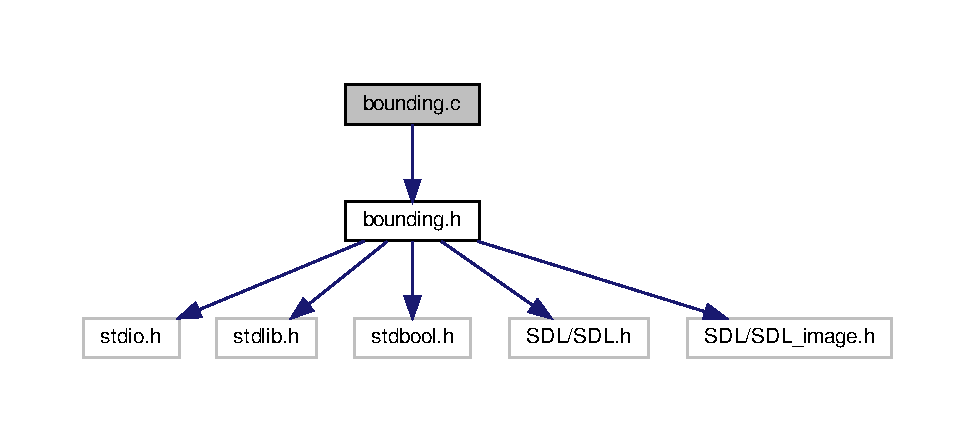
\includegraphics[width=350pt]{bounding_8c__incl}
\end{center}
\end{figure}
\subsection*{Functions}
\begin{DoxyCompactItemize}
\item 
bool \hyperlink{bounding_8c_a329bf2f9e06490e6864352e0d0deabba}{collision} (S\+D\+L\+\_\+\+Rect position1, S\+D\+L\+\_\+\+Rect position2)
\end{DoxyCompactItemize}


\subsection{Function Documentation}
\mbox{\Hypertarget{bounding_8c_a329bf2f9e06490e6864352e0d0deabba}\label{bounding_8c_a329bf2f9e06490e6864352e0d0deabba}} 
\index{bounding.\+c@{bounding.\+c}!collision@{collision}}
\index{collision@{collision}!bounding.\+c@{bounding.\+c}}
\subsubsection{\texorpdfstring{collision()}{collision()}}
{\footnotesize\ttfamily bool collision (\begin{DoxyParamCaption}\item[{S\+D\+L\+\_\+\+Rect}]{position1,  }\item[{S\+D\+L\+\_\+\+Rect}]{position2 }\end{DoxyParamCaption})}

Here is the caller graph for this function\+:\nopagebreak
\begin{figure}[H]
\begin{center}
\leavevmode
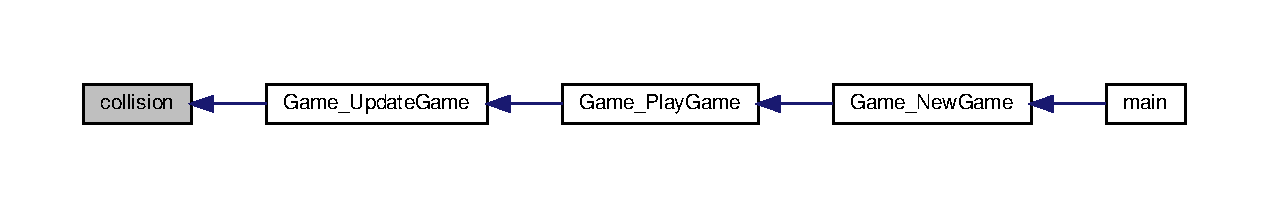
\includegraphics[width=350pt]{bounding_8c_a329bf2f9e06490e6864352e0d0deabba_icgraph}
\end{center}
\end{figure}

\hypertarget{bounding_8h}{}\section{bounding.\+h File Reference}
\label{bounding_8h}\index{bounding.\+h@{bounding.\+h}}
{\ttfamily \#include $<$stdio.\+h$>$}\newline
{\ttfamily \#include $<$stdlib.\+h$>$}\newline
{\ttfamily \#include $<$stdbool.\+h$>$}\newline
{\ttfamily \#include $<$S\+D\+L/\+S\+D\+L.\+h$>$}\newline
{\ttfamily \#include $<$S\+D\+L/\+S\+D\+L\+\_\+image.\+h$>$}\newline
Include dependency graph for bounding.\+h\+:\nopagebreak
\begin{figure}[H]
\begin{center}
\leavevmode
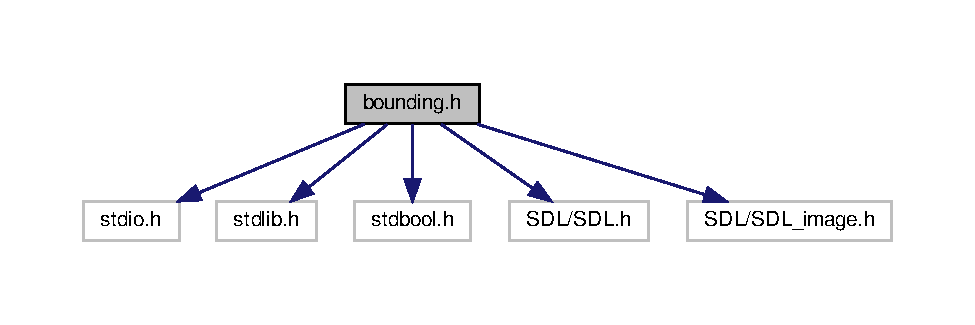
\includegraphics[width=350pt]{bounding_8h__incl}
\end{center}
\end{figure}
This graph shows which files directly or indirectly include this file\+:\nopagebreak
\begin{figure}[H]
\begin{center}
\leavevmode
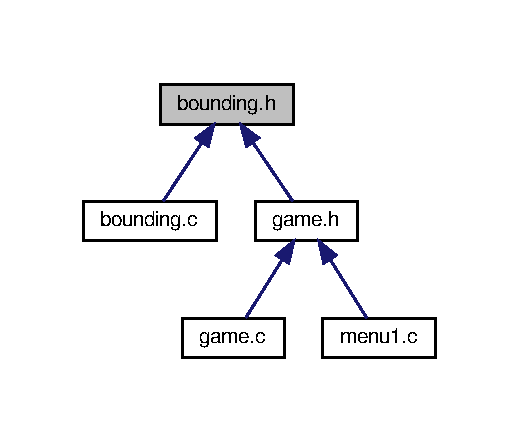
\includegraphics[width=249pt]{bounding_8h__dep__incl}
\end{center}
\end{figure}
\subsection*{Functions}
\begin{DoxyCompactItemize}
\item 
bool \hyperlink{bounding_8h_a329bf2f9e06490e6864352e0d0deabba}{collision} (S\+D\+L\+\_\+\+Rect position1, S\+D\+L\+\_\+\+Rect position2)
\end{DoxyCompactItemize}


\subsection{Function Documentation}
\mbox{\Hypertarget{bounding_8h_a329bf2f9e06490e6864352e0d0deabba}\label{bounding_8h_a329bf2f9e06490e6864352e0d0deabba}} 
\index{bounding.\+h@{bounding.\+h}!collision@{collision}}
\index{collision@{collision}!bounding.\+h@{bounding.\+h}}
\subsubsection{\texorpdfstring{collision()}{collision()}}
{\footnotesize\ttfamily bool collision (\begin{DoxyParamCaption}\item[{S\+D\+L\+\_\+\+Rect}]{position1,  }\item[{S\+D\+L\+\_\+\+Rect}]{position2 }\end{DoxyParamCaption})}

Here is the caller graph for this function\+:\nopagebreak
\begin{figure}[H]
\begin{center}
\leavevmode
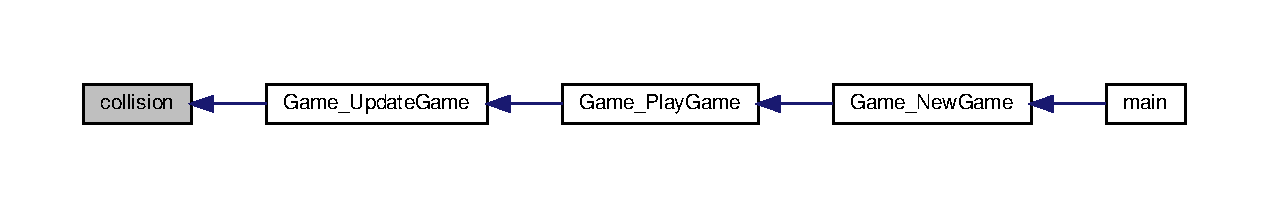
\includegraphics[width=350pt]{bounding_8h_a329bf2f9e06490e6864352e0d0deabba_icgraph}
\end{center}
\end{figure}

\hypertarget{chrono_8c}{}\section{chrono.\+c File Reference}
\label{chrono_8c}\index{chrono.\+c@{chrono.\+c}}
{\ttfamily \#include \char`\"{}chrono.\+h\char`\"{}}\newline
Include dependency graph for chrono.\+c\+:\nopagebreak
\begin{figure}[H]
\begin{center}
\leavevmode
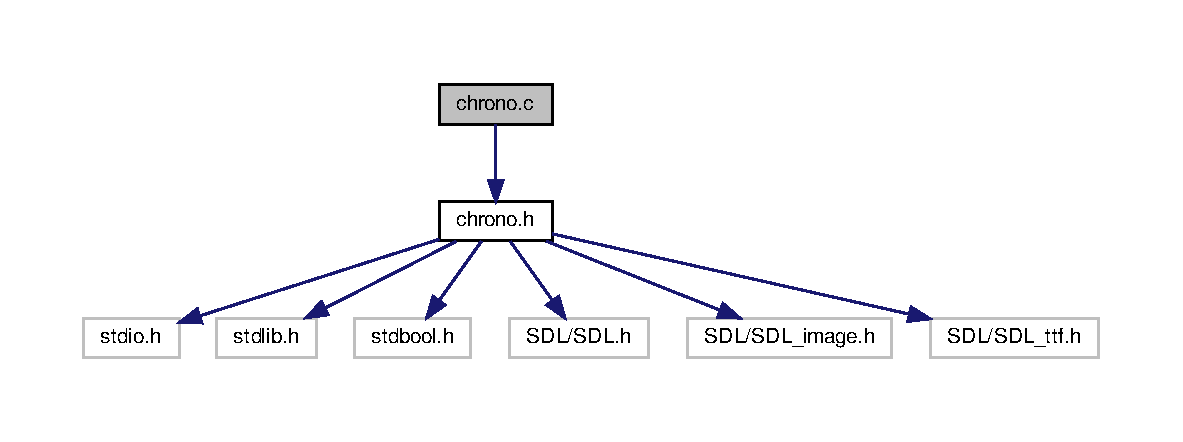
\includegraphics[width=350pt]{chrono_8c__incl}
\end{center}
\end{figure}
\subsection*{Functions}
\begin{DoxyCompactItemize}
\item 
void \hyperlink{chrono_8c_a4f18121f5be6b749338e124b619c98ef}{Init\+\_\+\+Chrono} (\hyperlink{structChrono}{Chrono} $\ast$c, S\+D\+L\+\_\+\+Rect pos, int temps)
\item 
void \hyperlink{chrono_8c_a0a7d9bb6ec2f958b0792124e90086eec}{Display\+\_\+\+Chrono} (\hyperlink{structChrono}{Chrono} $\ast$c, S\+D\+L\+\_\+\+Surface $\ast$ecran)
\item 
bool \hyperlink{chrono_8c_a49f308e7b7931061a6d9850365f262b2}{Calcul\+\_\+\+Chrono} (\hyperlink{structChrono}{Chrono} $\ast$c)
\item 
bool \hyperlink{chrono_8c_a70e794bee740ef0c7014ac453e0134d6}{Calcul\+\_\+\+ChronoE} (\hyperlink{structChrono}{Chrono} $\ast$c, S\+D\+L\+\_\+\+Surface $\ast$ecran)
\item 
void \hyperlink{chrono_8c_a56356592f0560380dceb270a7cfeaef1}{Pause\+\_\+\+Chrono} (\hyperlink{structChrono}{Chrono} $\ast$c)
\end{DoxyCompactItemize}


\subsection{Function Documentation}
\mbox{\Hypertarget{chrono_8c_a49f308e7b7931061a6d9850365f262b2}\label{chrono_8c_a49f308e7b7931061a6d9850365f262b2}} 
\index{chrono.\+c@{chrono.\+c}!Calcul\+\_\+\+Chrono@{Calcul\+\_\+\+Chrono}}
\index{Calcul\+\_\+\+Chrono@{Calcul\+\_\+\+Chrono}!chrono.\+c@{chrono.\+c}}
\subsubsection{\texorpdfstring{Calcul\+\_\+\+Chrono()}{Calcul\_Chrono()}}
{\footnotesize\ttfamily bool Calcul\+\_\+\+Chrono (\begin{DoxyParamCaption}\item[{\hyperlink{structChrono}{Chrono} $\ast$}]{c }\end{DoxyParamCaption})}

Here is the caller graph for this function\+:\nopagebreak
\begin{figure}[H]
\begin{center}
\leavevmode
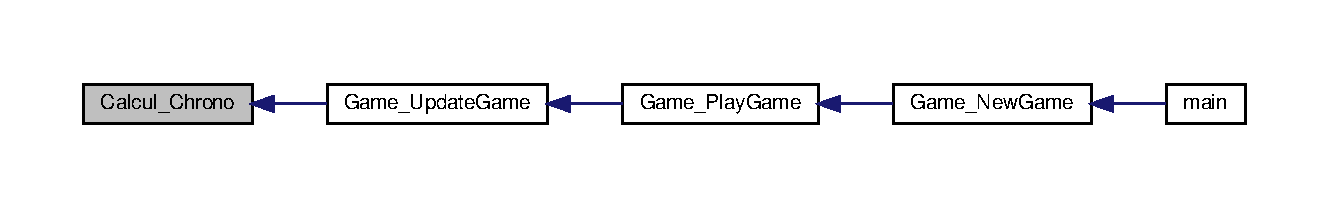
\includegraphics[width=350pt]{chrono_8c_a49f308e7b7931061a6d9850365f262b2_icgraph}
\end{center}
\end{figure}
\mbox{\Hypertarget{chrono_8c_a70e794bee740ef0c7014ac453e0134d6}\label{chrono_8c_a70e794bee740ef0c7014ac453e0134d6}} 
\index{chrono.\+c@{chrono.\+c}!Calcul\+\_\+\+ChronoE@{Calcul\+\_\+\+ChronoE}}
\index{Calcul\+\_\+\+ChronoE@{Calcul\+\_\+\+ChronoE}!chrono.\+c@{chrono.\+c}}
\subsubsection{\texorpdfstring{Calcul\+\_\+\+Chrono\+E()}{Calcul\_ChronoE()}}
{\footnotesize\ttfamily bool Calcul\+\_\+\+ChronoE (\begin{DoxyParamCaption}\item[{\hyperlink{structChrono}{Chrono} $\ast$}]{c,  }\item[{S\+D\+L\+\_\+\+Surface $\ast$}]{ecran }\end{DoxyParamCaption})}

\mbox{\Hypertarget{chrono_8c_a0a7d9bb6ec2f958b0792124e90086eec}\label{chrono_8c_a0a7d9bb6ec2f958b0792124e90086eec}} 
\index{chrono.\+c@{chrono.\+c}!Display\+\_\+\+Chrono@{Display\+\_\+\+Chrono}}
\index{Display\+\_\+\+Chrono@{Display\+\_\+\+Chrono}!chrono.\+c@{chrono.\+c}}
\subsubsection{\texorpdfstring{Display\+\_\+\+Chrono()}{Display\_Chrono()}}
{\footnotesize\ttfamily void Display\+\_\+\+Chrono (\begin{DoxyParamCaption}\item[{\hyperlink{structChrono}{Chrono} $\ast$}]{c,  }\item[{S\+D\+L\+\_\+\+Surface $\ast$}]{ecran }\end{DoxyParamCaption})}

Here is the caller graph for this function\+:\nopagebreak
\begin{figure}[H]
\begin{center}
\leavevmode
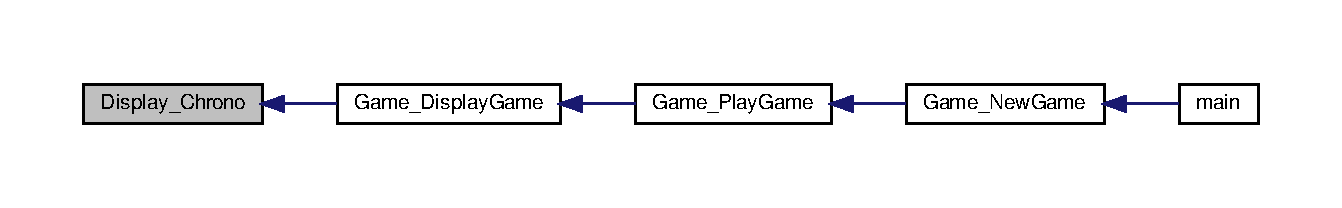
\includegraphics[width=350pt]{chrono_8c_a0a7d9bb6ec2f958b0792124e90086eec_icgraph}
\end{center}
\end{figure}
\mbox{\Hypertarget{chrono_8c_a4f18121f5be6b749338e124b619c98ef}\label{chrono_8c_a4f18121f5be6b749338e124b619c98ef}} 
\index{chrono.\+c@{chrono.\+c}!Init\+\_\+\+Chrono@{Init\+\_\+\+Chrono}}
\index{Init\+\_\+\+Chrono@{Init\+\_\+\+Chrono}!chrono.\+c@{chrono.\+c}}
\subsubsection{\texorpdfstring{Init\+\_\+\+Chrono()}{Init\_Chrono()}}
{\footnotesize\ttfamily void Init\+\_\+\+Chrono (\begin{DoxyParamCaption}\item[{\hyperlink{structChrono}{Chrono} $\ast$}]{c,  }\item[{S\+D\+L\+\_\+\+Rect}]{pos,  }\item[{int}]{temps }\end{DoxyParamCaption})}

Here is the caller graph for this function\+:\nopagebreak
\begin{figure}[H]
\begin{center}
\leavevmode
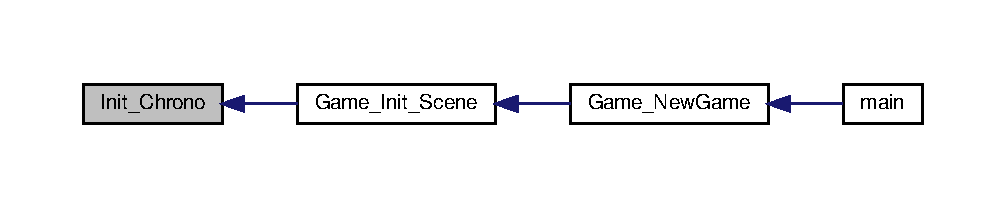
\includegraphics[width=350pt]{chrono_8c_a4f18121f5be6b749338e124b619c98ef_icgraph}
\end{center}
\end{figure}
\mbox{\Hypertarget{chrono_8c_a56356592f0560380dceb270a7cfeaef1}\label{chrono_8c_a56356592f0560380dceb270a7cfeaef1}} 
\index{chrono.\+c@{chrono.\+c}!Pause\+\_\+\+Chrono@{Pause\+\_\+\+Chrono}}
\index{Pause\+\_\+\+Chrono@{Pause\+\_\+\+Chrono}!chrono.\+c@{chrono.\+c}}
\subsubsection{\texorpdfstring{Pause\+\_\+\+Chrono()}{Pause\_Chrono()}}
{\footnotesize\ttfamily void Pause\+\_\+\+Chrono (\begin{DoxyParamCaption}\item[{\hyperlink{structChrono}{Chrono} $\ast$}]{c }\end{DoxyParamCaption})}

Here is the caller graph for this function\+:\nopagebreak
\begin{figure}[H]
\begin{center}
\leavevmode
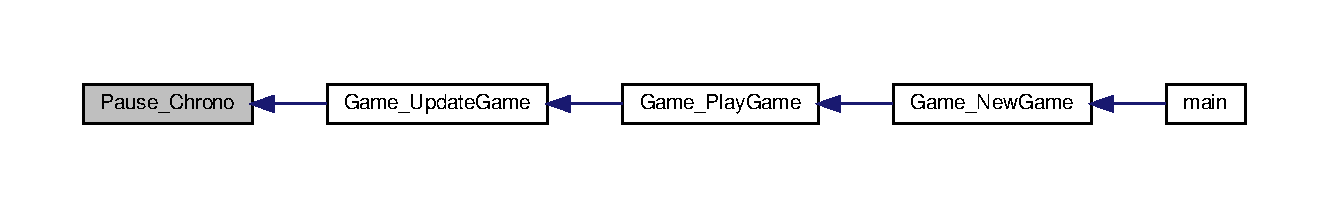
\includegraphics[width=350pt]{chrono_8c_a56356592f0560380dceb270a7cfeaef1_icgraph}
\end{center}
\end{figure}

\hypertarget{chrono_8h}{}\section{chrono.\+h File Reference}
\label{chrono_8h}\index{chrono.\+h@{chrono.\+h}}
{\ttfamily \#include $<$stdio.\+h$>$}\newline
{\ttfamily \#include $<$stdlib.\+h$>$}\newline
{\ttfamily \#include $<$stdbool.\+h$>$}\newline
{\ttfamily \#include $<$S\+D\+L/\+S\+D\+L.\+h$>$}\newline
{\ttfamily \#include $<$S\+D\+L/\+S\+D\+L\+\_\+image.\+h$>$}\newline
{\ttfamily \#include $<$S\+D\+L/\+S\+D\+L\+\_\+ttf.\+h$>$}\newline
Include dependency graph for chrono.\+h\+:\nopagebreak
\begin{figure}[H]
\begin{center}
\leavevmode
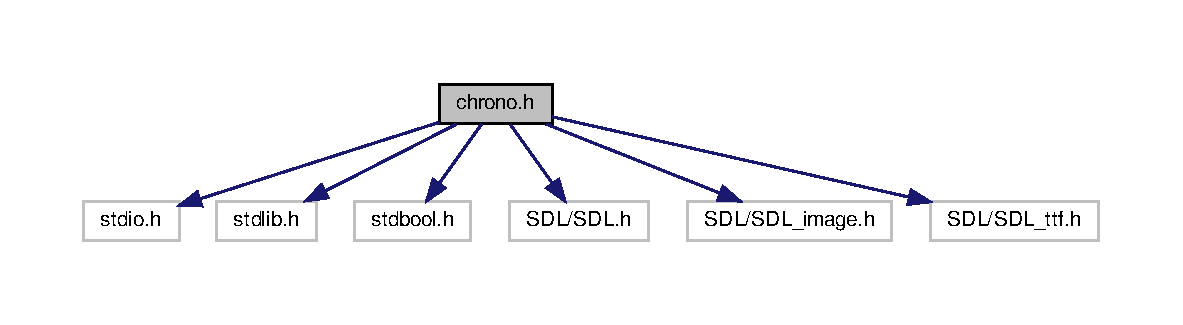
\includegraphics[width=350pt]{chrono_8h__incl}
\end{center}
\end{figure}
This graph shows which files directly or indirectly include this file\+:\nopagebreak
\begin{figure}[H]
\begin{center}
\leavevmode
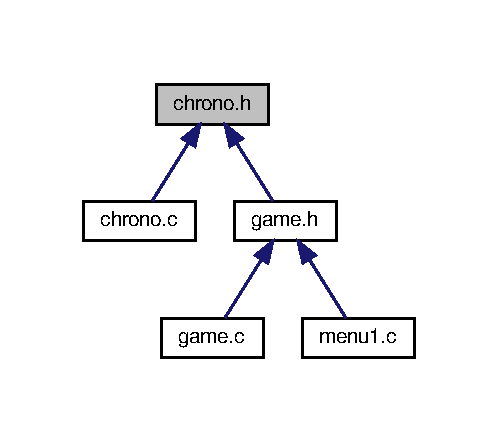
\includegraphics[width=239pt]{chrono_8h__dep__incl}
\end{center}
\end{figure}
\subsection*{Data Structures}
\begin{DoxyCompactItemize}
\item 
struct \hyperlink{structChrono}{Chrono}
\end{DoxyCompactItemize}
\subsection*{Functions}
\begin{DoxyCompactItemize}
\item 
void \hyperlink{chrono_8h_a4f18121f5be6b749338e124b619c98ef}{Init\+\_\+\+Chrono} (\hyperlink{structChrono}{Chrono} $\ast$c, S\+D\+L\+\_\+\+Rect pos, int temps)
\item 
void \hyperlink{chrono_8h_a0a7d9bb6ec2f958b0792124e90086eec}{Display\+\_\+\+Chrono} (\hyperlink{structChrono}{Chrono} $\ast$c, S\+D\+L\+\_\+\+Surface $\ast$ecran)
\item 
bool \hyperlink{chrono_8h_a49f308e7b7931061a6d9850365f262b2}{Calcul\+\_\+\+Chrono} (\hyperlink{structChrono}{Chrono} $\ast$c)
\item 
void \hyperlink{chrono_8h_a56356592f0560380dceb270a7cfeaef1}{Pause\+\_\+\+Chrono} (\hyperlink{structChrono}{Chrono} $\ast$c)
\item 
bool \hyperlink{chrono_8h_a70e794bee740ef0c7014ac453e0134d6}{Calcul\+\_\+\+ChronoE} (\hyperlink{structChrono}{Chrono} $\ast$c, S\+D\+L\+\_\+\+Surface $\ast$ecran)
\end{DoxyCompactItemize}


\subsection{Function Documentation}
\mbox{\Hypertarget{chrono_8h_a49f308e7b7931061a6d9850365f262b2}\label{chrono_8h_a49f308e7b7931061a6d9850365f262b2}} 
\index{chrono.\+h@{chrono.\+h}!Calcul\+\_\+\+Chrono@{Calcul\+\_\+\+Chrono}}
\index{Calcul\+\_\+\+Chrono@{Calcul\+\_\+\+Chrono}!chrono.\+h@{chrono.\+h}}
\subsubsection{\texorpdfstring{Calcul\+\_\+\+Chrono()}{Calcul\_Chrono()}}
{\footnotesize\ttfamily bool Calcul\+\_\+\+Chrono (\begin{DoxyParamCaption}\item[{\hyperlink{structChrono}{Chrono} $\ast$}]{c }\end{DoxyParamCaption})}

Here is the caller graph for this function\+:\nopagebreak
\begin{figure}[H]
\begin{center}
\leavevmode
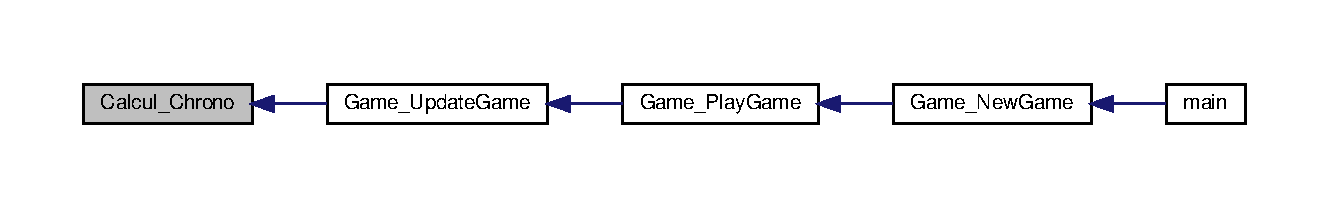
\includegraphics[width=350pt]{chrono_8h_a49f308e7b7931061a6d9850365f262b2_icgraph}
\end{center}
\end{figure}
\mbox{\Hypertarget{chrono_8h_a70e794bee740ef0c7014ac453e0134d6}\label{chrono_8h_a70e794bee740ef0c7014ac453e0134d6}} 
\index{chrono.\+h@{chrono.\+h}!Calcul\+\_\+\+ChronoE@{Calcul\+\_\+\+ChronoE}}
\index{Calcul\+\_\+\+ChronoE@{Calcul\+\_\+\+ChronoE}!chrono.\+h@{chrono.\+h}}
\subsubsection{\texorpdfstring{Calcul\+\_\+\+Chrono\+E()}{Calcul\_ChronoE()}}
{\footnotesize\ttfamily bool Calcul\+\_\+\+ChronoE (\begin{DoxyParamCaption}\item[{\hyperlink{structChrono}{Chrono} $\ast$}]{c,  }\item[{S\+D\+L\+\_\+\+Surface $\ast$}]{ecran }\end{DoxyParamCaption})}

\mbox{\Hypertarget{chrono_8h_a0a7d9bb6ec2f958b0792124e90086eec}\label{chrono_8h_a0a7d9bb6ec2f958b0792124e90086eec}} 
\index{chrono.\+h@{chrono.\+h}!Display\+\_\+\+Chrono@{Display\+\_\+\+Chrono}}
\index{Display\+\_\+\+Chrono@{Display\+\_\+\+Chrono}!chrono.\+h@{chrono.\+h}}
\subsubsection{\texorpdfstring{Display\+\_\+\+Chrono()}{Display\_Chrono()}}
{\footnotesize\ttfamily void Display\+\_\+\+Chrono (\begin{DoxyParamCaption}\item[{\hyperlink{structChrono}{Chrono} $\ast$}]{c,  }\item[{S\+D\+L\+\_\+\+Surface $\ast$}]{ecran }\end{DoxyParamCaption})}

Here is the caller graph for this function\+:\nopagebreak
\begin{figure}[H]
\begin{center}
\leavevmode
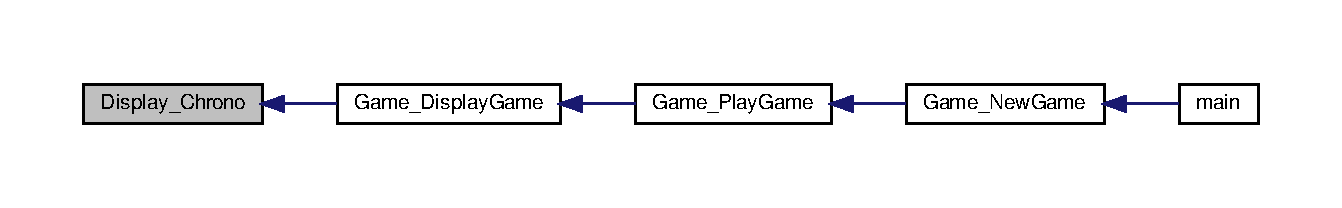
\includegraphics[width=350pt]{chrono_8h_a0a7d9bb6ec2f958b0792124e90086eec_icgraph}
\end{center}
\end{figure}
\mbox{\Hypertarget{chrono_8h_a4f18121f5be6b749338e124b619c98ef}\label{chrono_8h_a4f18121f5be6b749338e124b619c98ef}} 
\index{chrono.\+h@{chrono.\+h}!Init\+\_\+\+Chrono@{Init\+\_\+\+Chrono}}
\index{Init\+\_\+\+Chrono@{Init\+\_\+\+Chrono}!chrono.\+h@{chrono.\+h}}
\subsubsection{\texorpdfstring{Init\+\_\+\+Chrono()}{Init\_Chrono()}}
{\footnotesize\ttfamily void Init\+\_\+\+Chrono (\begin{DoxyParamCaption}\item[{\hyperlink{structChrono}{Chrono} $\ast$}]{c,  }\item[{S\+D\+L\+\_\+\+Rect}]{pos,  }\item[{int}]{temps }\end{DoxyParamCaption})}

Here is the caller graph for this function\+:\nopagebreak
\begin{figure}[H]
\begin{center}
\leavevmode
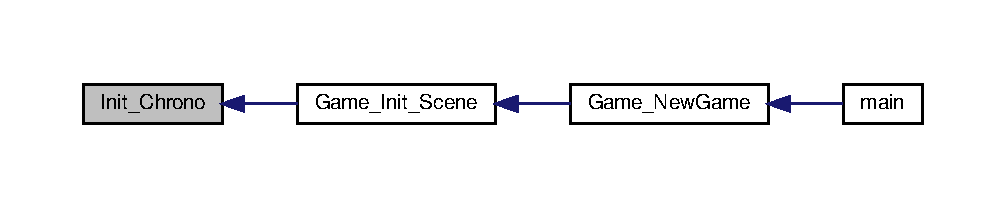
\includegraphics[width=350pt]{chrono_8h_a4f18121f5be6b749338e124b619c98ef_icgraph}
\end{center}
\end{figure}
\mbox{\Hypertarget{chrono_8h_a56356592f0560380dceb270a7cfeaef1}\label{chrono_8h_a56356592f0560380dceb270a7cfeaef1}} 
\index{chrono.\+h@{chrono.\+h}!Pause\+\_\+\+Chrono@{Pause\+\_\+\+Chrono}}
\index{Pause\+\_\+\+Chrono@{Pause\+\_\+\+Chrono}!chrono.\+h@{chrono.\+h}}
\subsubsection{\texorpdfstring{Pause\+\_\+\+Chrono()}{Pause\_Chrono()}}
{\footnotesize\ttfamily void Pause\+\_\+\+Chrono (\begin{DoxyParamCaption}\item[{\hyperlink{structChrono}{Chrono} $\ast$}]{c }\end{DoxyParamCaption})}

Here is the caller graph for this function\+:\nopagebreak
\begin{figure}[H]
\begin{center}
\leavevmode
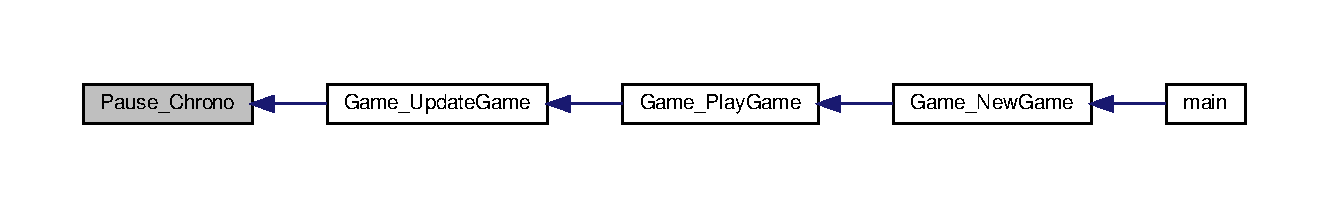
\includegraphics[width=350pt]{chrono_8h_a56356592f0560380dceb270a7cfeaef1_icgraph}
\end{center}
\end{figure}

\hypertarget{chronometre_8c}{}\section{chronometre.\+c File Reference}
\label{chronometre_8c}\index{chronometre.\+c@{chronometre.\+c}}
\subsection*{Functions}
\begin{DoxyCompactItemize}
\item 
clock\+\_\+t \hyperlink{chronometre_8c_ab731f86a58ec470cb9584a5502440645}{initchrono} ()
\item 
int \hyperlink{chronometre_8c_ad35041ee3fd517e90dc82bda7b94e17a}{chrono} (int debut)
\end{DoxyCompactItemize}


\subsection{Function Documentation}
\mbox{\Hypertarget{chronometre_8c_ad35041ee3fd517e90dc82bda7b94e17a}\label{chronometre_8c_ad35041ee3fd517e90dc82bda7b94e17a}} 
\index{chronometre.\+c@{chronometre.\+c}!chrono@{chrono}}
\index{chrono@{chrono}!chronometre.\+c@{chronometre.\+c}}
\subsubsection{\texorpdfstring{chrono()}{chrono()}}
{\footnotesize\ttfamily int chrono (\begin{DoxyParamCaption}\item[{int}]{debut }\end{DoxyParamCaption})}

\mbox{\Hypertarget{chronometre_8c_ab731f86a58ec470cb9584a5502440645}\label{chronometre_8c_ab731f86a58ec470cb9584a5502440645}} 
\index{chronometre.\+c@{chronometre.\+c}!initchrono@{initchrono}}
\index{initchrono@{initchrono}!chronometre.\+c@{chronometre.\+c}}
\subsubsection{\texorpdfstring{initchrono()}{initchrono()}}
{\footnotesize\ttfamily clock\+\_\+t initchrono (\begin{DoxyParamCaption}{ }\end{DoxyParamCaption})}


\hypertarget{collisionparfait_8c}{}\section{collisionparfait.\+c File Reference}
\label{collisionparfait_8c}\index{collisionparfait.\+c@{collisionparfait.\+c}}
{\ttfamily \#include \char`\"{}collisionparfait.\+h\char`\"{}}\newline
Include dependency graph for collisionparfait.\+c\+:\nopagebreak
\begin{figure}[H]
\begin{center}
\leavevmode
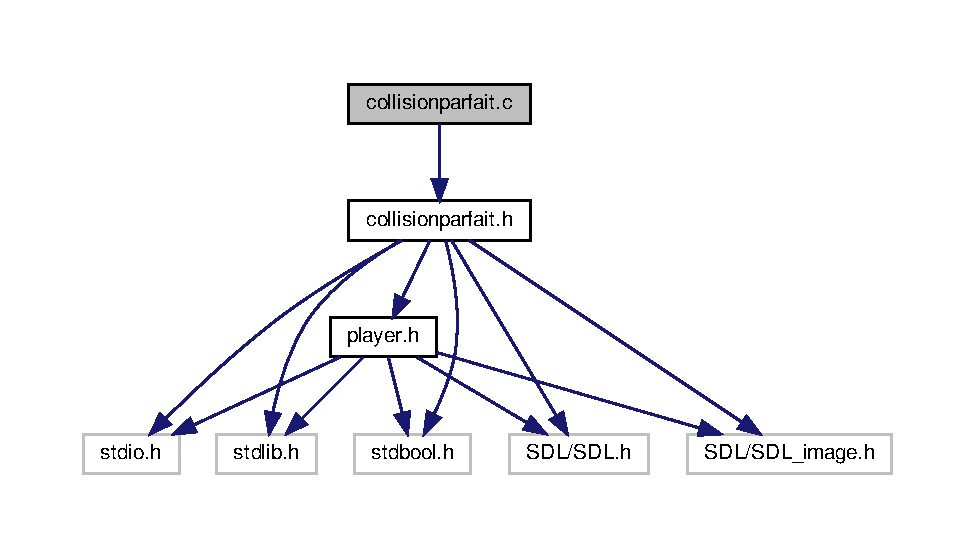
\includegraphics[width=350pt]{collisionparfait_8c__incl}
\end{center}
\end{figure}
\subsection*{Functions}
\begin{DoxyCompactItemize}
\item 
S\+D\+L\+\_\+\+Color \hyperlink{collisionparfait_8c_a9ec79b71532402381966fc93325d3e52}{Get\+Pixel} (S\+D\+L\+\_\+\+Surface $\ast$p\+Surface, int x, int y)
\item 
int \hyperlink{collisionparfait_8c_a4cb9ad745cdcc0c1f45f6adc0739156f}{Collision\+\_\+\+Parfait} (\hyperlink{structPlayer}{Player} $\ast$p, S\+D\+L\+\_\+\+Surface $\ast$background\+Mask)
\end{DoxyCompactItemize}


\subsection{Function Documentation}
\mbox{\Hypertarget{collisionparfait_8c_a4cb9ad745cdcc0c1f45f6adc0739156f}\label{collisionparfait_8c_a4cb9ad745cdcc0c1f45f6adc0739156f}} 
\index{collisionparfait.\+c@{collisionparfait.\+c}!Collision\+\_\+\+Parfait@{Collision\+\_\+\+Parfait}}
\index{Collision\+\_\+\+Parfait@{Collision\+\_\+\+Parfait}!collisionparfait.\+c@{collisionparfait.\+c}}
\subsubsection{\texorpdfstring{Collision\+\_\+\+Parfait()}{Collision\_Parfait()}}
{\footnotesize\ttfamily int Collision\+\_\+\+Parfait (\begin{DoxyParamCaption}\item[{\hyperlink{structPlayer}{Player} $\ast$}]{p,  }\item[{S\+D\+L\+\_\+\+Surface $\ast$}]{background\+Mask }\end{DoxyParamCaption})}

Here is the call graph for this function\+:\nopagebreak
\begin{figure}[H]
\begin{center}
\leavevmode
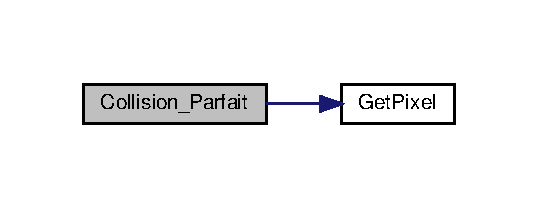
\includegraphics[width=258pt]{collisionparfait_8c_a4cb9ad745cdcc0c1f45f6adc0739156f_cgraph}
\end{center}
\end{figure}
Here is the caller graph for this function\+:\nopagebreak
\begin{figure}[H]
\begin{center}
\leavevmode
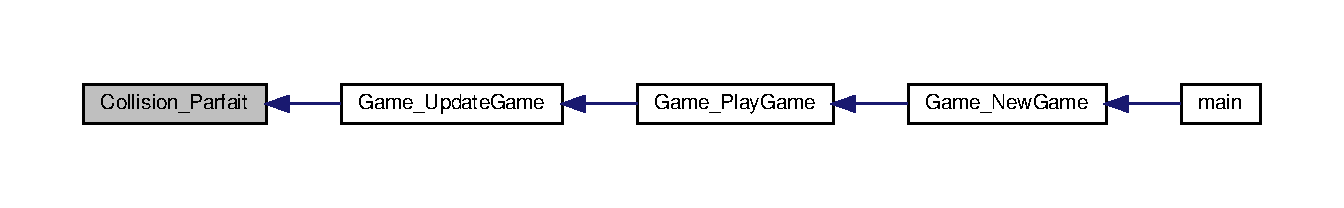
\includegraphics[width=350pt]{collisionparfait_8c_a4cb9ad745cdcc0c1f45f6adc0739156f_icgraph}
\end{center}
\end{figure}
\mbox{\Hypertarget{collisionparfait_8c_a9ec79b71532402381966fc93325d3e52}\label{collisionparfait_8c_a9ec79b71532402381966fc93325d3e52}} 
\index{collisionparfait.\+c@{collisionparfait.\+c}!Get\+Pixel@{Get\+Pixel}}
\index{Get\+Pixel@{Get\+Pixel}!collisionparfait.\+c@{collisionparfait.\+c}}
\subsubsection{\texorpdfstring{Get\+Pixel()}{GetPixel()}}
{\footnotesize\ttfamily S\+D\+L\+\_\+\+Color Get\+Pixel (\begin{DoxyParamCaption}\item[{S\+D\+L\+\_\+\+Surface $\ast$}]{p\+Surface,  }\item[{int}]{x,  }\item[{int}]{y }\end{DoxyParamCaption})}

Here is the caller graph for this function\+:\nopagebreak
\begin{figure}[H]
\begin{center}
\leavevmode
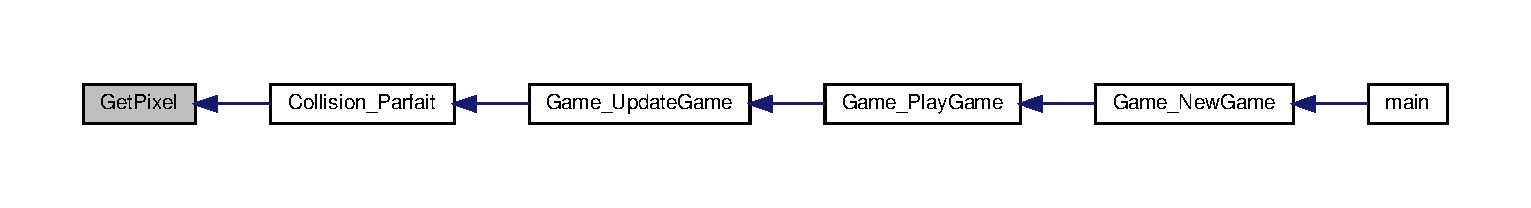
\includegraphics[width=350pt]{collisionparfait_8c_a9ec79b71532402381966fc93325d3e52_icgraph}
\end{center}
\end{figure}

\hypertarget{collisionparfait_8h}{}\section{collisionparfait.\+h File Reference}
\label{collisionparfait_8h}\index{collisionparfait.\+h@{collisionparfait.\+h}}
{\ttfamily \#include $<$stdio.\+h$>$}\newline
{\ttfamily \#include $<$stdlib.\+h$>$}\newline
{\ttfamily \#include $<$stdbool.\+h$>$}\newline
{\ttfamily \#include $<$S\+D\+L/\+S\+D\+L.\+h$>$}\newline
{\ttfamily \#include $<$S\+D\+L/\+S\+D\+L\+\_\+image.\+h$>$}\newline
{\ttfamily \#include \char`\"{}player.\+h\char`\"{}}\newline
Include dependency graph for collisionparfait.\+h\+:\nopagebreak
\begin{figure}[H]
\begin{center}
\leavevmode
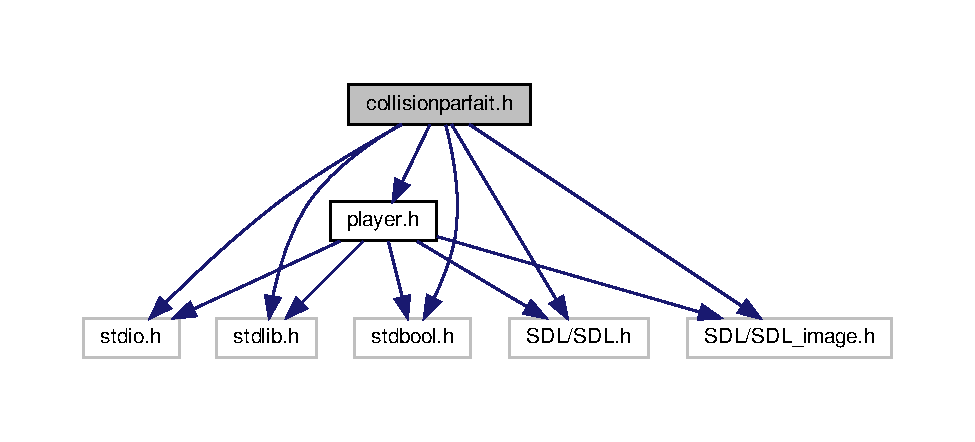
\includegraphics[width=350pt]{collisionparfait_8h__incl}
\end{center}
\end{figure}
This graph shows which files directly or indirectly include this file\+:\nopagebreak
\begin{figure}[H]
\begin{center}
\leavevmode
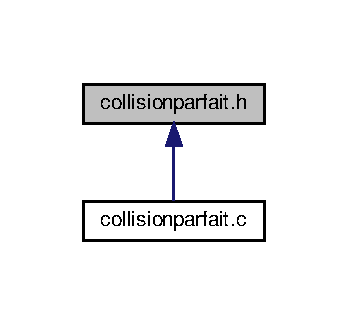
\includegraphics[width=167pt]{collisionparfait_8h__dep__incl}
\end{center}
\end{figure}
\subsection*{Functions}
\begin{DoxyCompactItemize}
\item 
S\+D\+L\+\_\+\+Color \hyperlink{collisionparfait_8h_a9ec79b71532402381966fc93325d3e52}{Get\+Pixel} (S\+D\+L\+\_\+\+Surface $\ast$p\+Surface, int x, int y)
\item 
int \hyperlink{collisionparfait_8h_a4cb9ad745cdcc0c1f45f6adc0739156f}{Collision\+\_\+\+Parfait} (\hyperlink{structPlayer}{Player} $\ast$p, S\+D\+L\+\_\+\+Surface $\ast$background\+Mask)
\end{DoxyCompactItemize}


\subsection{Function Documentation}
\mbox{\Hypertarget{collisionparfait_8h_a4cb9ad745cdcc0c1f45f6adc0739156f}\label{collisionparfait_8h_a4cb9ad745cdcc0c1f45f6adc0739156f}} 
\index{collisionparfait.\+h@{collisionparfait.\+h}!Collision\+\_\+\+Parfait@{Collision\+\_\+\+Parfait}}
\index{Collision\+\_\+\+Parfait@{Collision\+\_\+\+Parfait}!collisionparfait.\+h@{collisionparfait.\+h}}
\subsubsection{\texorpdfstring{Collision\+\_\+\+Parfait()}{Collision\_Parfait()}}
{\footnotesize\ttfamily int Collision\+\_\+\+Parfait (\begin{DoxyParamCaption}\item[{\hyperlink{structPlayer}{Player} $\ast$}]{p,  }\item[{S\+D\+L\+\_\+\+Surface $\ast$}]{background\+Mask }\end{DoxyParamCaption})}

Here is the call graph for this function\+:\nopagebreak
\begin{figure}[H]
\begin{center}
\leavevmode
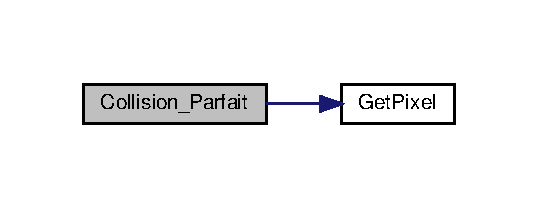
\includegraphics[width=258pt]{collisionparfait_8h_a4cb9ad745cdcc0c1f45f6adc0739156f_cgraph}
\end{center}
\end{figure}
Here is the caller graph for this function\+:\nopagebreak
\begin{figure}[H]
\begin{center}
\leavevmode
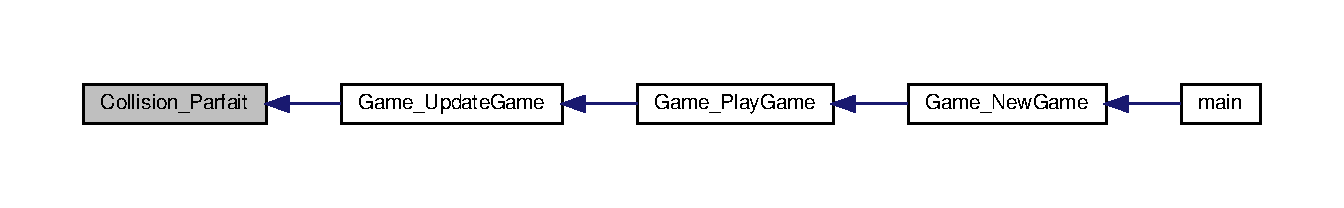
\includegraphics[width=350pt]{collisionparfait_8h_a4cb9ad745cdcc0c1f45f6adc0739156f_icgraph}
\end{center}
\end{figure}
\mbox{\Hypertarget{collisionparfait_8h_a9ec79b71532402381966fc93325d3e52}\label{collisionparfait_8h_a9ec79b71532402381966fc93325d3e52}} 
\index{collisionparfait.\+h@{collisionparfait.\+h}!Get\+Pixel@{Get\+Pixel}}
\index{Get\+Pixel@{Get\+Pixel}!collisionparfait.\+h@{collisionparfait.\+h}}
\subsubsection{\texorpdfstring{Get\+Pixel()}{GetPixel()}}
{\footnotesize\ttfamily S\+D\+L\+\_\+\+Color Get\+Pixel (\begin{DoxyParamCaption}\item[{S\+D\+L\+\_\+\+Surface $\ast$}]{p\+Surface,  }\item[{int}]{x,  }\item[{int}]{y }\end{DoxyParamCaption})}

Here is the caller graph for this function\+:\nopagebreak
\begin{figure}[H]
\begin{center}
\leavevmode
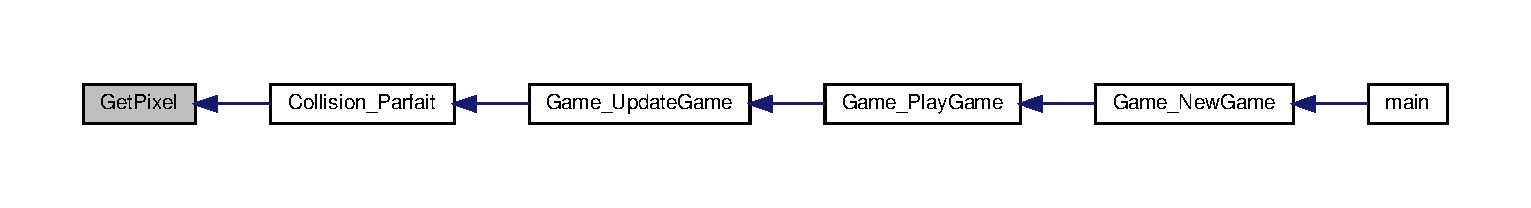
\includegraphics[width=350pt]{collisionparfait_8h_a9ec79b71532402381966fc93325d3e52_icgraph}
\end{center}
\end{figure}

\hypertarget{enigme1_8c}{}\section{enigme1.\+c File Reference}
\label{enigme1_8c}\index{enigme1.\+c@{enigme1.\+c}}
{\ttfamily \#include $<$stdlib.\+h$>$}\newline
{\ttfamily \#include $<$stdio.\+h$>$}\newline
{\ttfamily \#include $<$time.\+h$>$}\newline
{\ttfamily \#include $<$S\+D\+L/\+S\+D\+L.\+h$>$}\newline
{\ttfamily \#include $<$S\+D\+L/\+S\+D\+L\+\_\+ttf.\+h$>$}\newline
{\ttfamily \#include $<$S\+D\+L/\+S\+D\+L\+\_\+image.\+h$>$}\newline
{\ttfamily \#include $<$S\+D\+L/\+S\+D\+L\+\_\+mixer.\+h$>$}\newline
{\ttfamily \#include \char`\"{}fonctions.\+h\char`\"{}}\newline
Include dependency graph for enigme1.\+c\+:\nopagebreak
\begin{figure}[H]
\begin{center}
\leavevmode
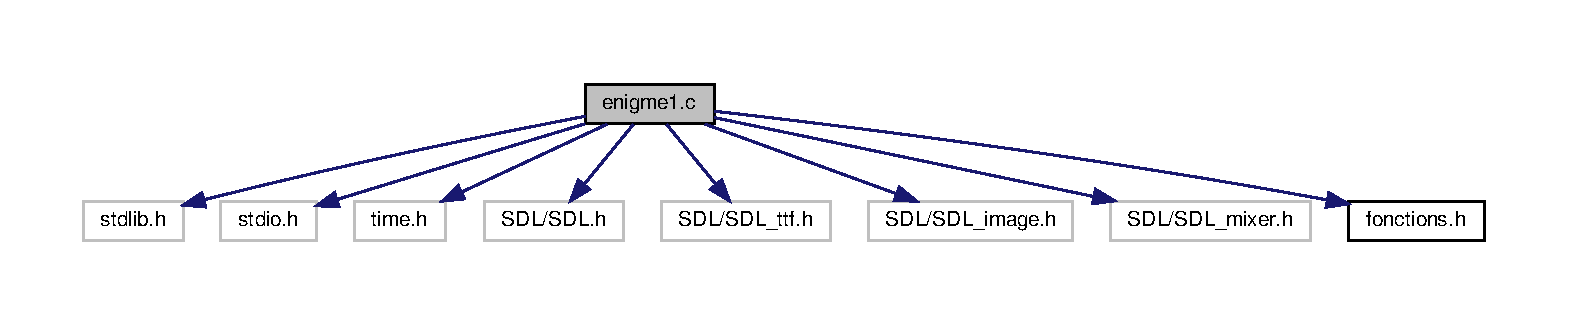
\includegraphics[width=350pt]{enigme1_8c__incl}
\end{center}
\end{figure}
\subsection*{Functions}
\begin{DoxyCompactItemize}
\item 
int \hyperlink{enigme1_8c_a0ddf1224851353fc92bfbff6f499fa97}{main} (int argc, char $\ast$argv\mbox{[}$\,$\mbox{]})
\end{DoxyCompactItemize}


\subsection{Function Documentation}
\mbox{\Hypertarget{enigme1_8c_a0ddf1224851353fc92bfbff6f499fa97}\label{enigme1_8c_a0ddf1224851353fc92bfbff6f499fa97}} 
\index{enigme1.\+c@{enigme1.\+c}!main@{main}}
\index{main@{main}!enigme1.\+c@{enigme1.\+c}}
\subsubsection{\texorpdfstring{main()}{main()}}
{\footnotesize\ttfamily int main (\begin{DoxyParamCaption}\item[{int}]{argc,  }\item[{char $\ast$}]{argv\mbox{[}$\,$\mbox{]} }\end{DoxyParamCaption})}

Here is the call graph for this function\+:\nopagebreak
\begin{figure}[H]
\begin{center}
\leavevmode
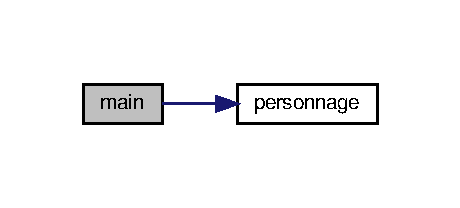
\includegraphics[width=221pt]{enigme1_8c_a0ddf1224851353fc92bfbff6f499fa97_cgraph}
\end{center}
\end{figure}

\hypertarget{enigmes_8c}{}\section{enigmes.\+c File Reference}
\label{enigmes_8c}\index{enigmes.\+c@{enigmes.\+c}}


toutes les enigmes  


{\ttfamily \#include $<$stdlib.\+h$>$}\newline
{\ttfamily \#include $<$stdio.\+h$>$}\newline
{\ttfamily \#include $<$time.\+h$>$}\newline
{\ttfamily \#include $<$S\+D\+L/\+S\+D\+L.\+h$>$}\newline
{\ttfamily \#include $<$S\+D\+L/\+S\+D\+L\+\_\+ttf.\+h$>$}\newline
{\ttfamily \#include $<$S\+D\+L/\+S\+D\+L\+\_\+image.\+h$>$}\newline
{\ttfamily \#include $<$S\+D\+L/\+S\+D\+L\+\_\+mixer.\+h$>$}\newline
{\ttfamily \#include \char`\"{}fonctions.\+h\char`\"{}}\newline
{\ttfamily \#include \char`\"{}enigmes.\+h\char`\"{}}\newline
Include dependency graph for enigmes.\+c\+:
\nopagebreak
\begin{figure}[H]
\begin{center}
\leavevmode
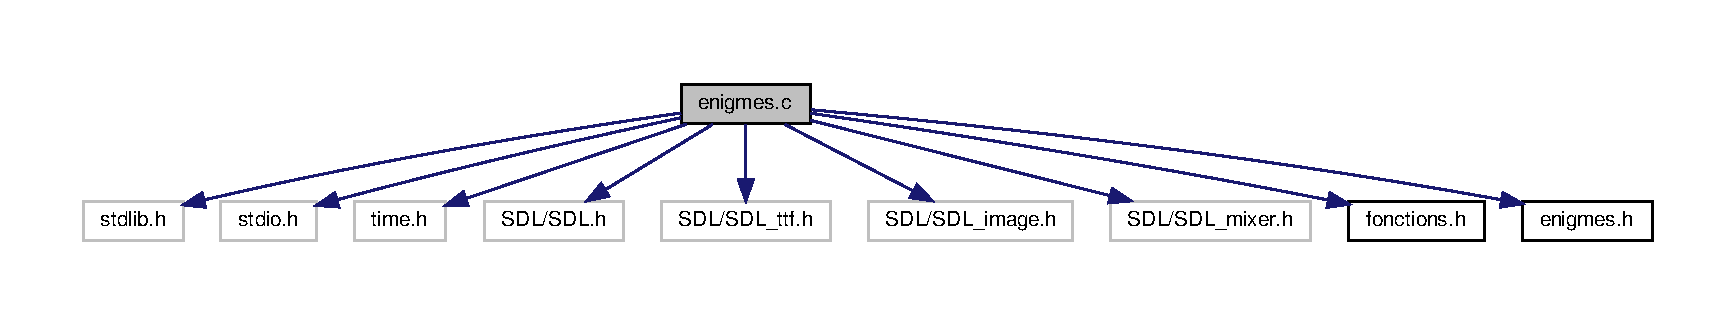
\includegraphics[width=350pt]{enigmes_8c__incl}
\end{center}
\end{figure}
\subsection*{Functions}
\begin{DoxyCompactItemize}
\item 
int \hyperlink{enigmes_8c_a07b23a568fbbfcff4c680d4c6af1820a}{enigme1} (S\+D\+L\+\_\+\+Surface $\ast$screen)
\begin{DoxyCompactList}\small\item\em pour enigme4 \end{DoxyCompactList}\item 
int \hyperlink{enigmes_8c_ae0f19513f31cfa44736ddefbb15a9a3a}{enigme2} (S\+D\+L\+\_\+\+Surface $\ast$screen)
\begin{DoxyCompactList}\small\item\em enigme 1 math random \end{DoxyCompactList}\item 
int \hyperlink{enigmes_8c_a8dbe78bd6afb9a66a8f8b768bdf7110b}{enigme3} (S\+D\+L\+\_\+\+Surface $\ast$screen)
\begin{DoxyCompactList}\small\item\em enigme 2 panda \end{DoxyCompactList}\item 
void \hyperlink{enigmes_8c_abc41653829a3c89b3907cd3ae5927145}{afficherenigme} (S\+D\+L\+\_\+\+Surface $\ast$screen, char $\ast$a)
\item 
int \hyperlink{enigmes_8c_a6cd927b8211a7ff6445f6dbdeed60413}{resolutionenigme} (int resultat, int resultat2)
\begin{DoxyCompactList}\small\item\em affichage enigme \end{DoxyCompactList}\item 
clock\+\_\+t \hyperlink{enigmes_8c_a6dd29323933d67965cc4741c9c0b0afa}{initchrono} (T\+T\+F\+\_\+\+Font $\ast$$\ast$police, S\+D\+L\+\_\+\+Surface $\ast$$\ast$black)
\begin{DoxyCompactList}\small\item\em resultat enigme \end{DoxyCompactList}\item 
int \hyperlink{enigmes_8c_adc73189bfe920e89bc93d37de8cf28f0}{chrono} (clock\+\_\+t debut, S\+D\+L\+\_\+\+Surface $\ast$screen, T\+T\+F\+\_\+\+Font $\ast$police, S\+D\+L\+\_\+\+Surface $\ast$black)
\begin{DoxyCompactList}\small\item\em initialisation du chronometre pour les enigmes \end{DoxyCompactList}\item 
int \hyperlink{enigmes_8c_a3a045cebb7e3097603076d550132c6a5}{updatesticks} (int sticks, S\+D\+L\+\_\+\+Surface $\ast$screen, T\+T\+F\+\_\+\+Font $\ast$police, S\+D\+L\+\_\+\+Surface $\ast$black, int choix)
\begin{DoxyCompactList}\small\item\em l\textquotesingle{}affichage du chronometre \end{DoxyCompactList}\item 
int \hyperlink{enigmes_8c_acae9a098bc124f835a2f5fd4aecee435}{winlose} (S\+D\+L\+\_\+\+Surface $\ast$screen, int player, S\+D\+L\+\_\+\+Surface $\ast$win, S\+D\+L\+\_\+\+Surface $\ast$lose, S\+D\+L\+\_\+\+Surface $\ast$rules, S\+D\+L\+\_\+\+Surface $\ast$continu\mbox{[}$\,$\mbox{]}, S\+D\+L\+\_\+\+Rect position, int $\ast$lvl)
\begin{DoxyCompactList}\small\item\em pour l enigme4 \end{DoxyCompactList}\item 
int \hyperlink{enigmes_8c_a9548e307594e7aa6d2cdbbcbb4156524}{enigme4} (S\+D\+L\+\_\+\+Surface $\ast$screen)
\begin{DoxyCompactList}\small\item\em enigme 3 des question apartir d\textquotesingle{}un fichier \end{DoxyCompactList}\end{DoxyCompactItemize}


\subsection{Detailed Description}
toutes les enigmes 

\begin{DoxyAuthor}{Author}
Mohamed Ali Bouzaiene 
\end{DoxyAuthor}
\begin{DoxyVersion}{Version}
0.\+0.\+1 
\end{DoxyVersion}


\subsection{Function Documentation}
\mbox{\Hypertarget{enigmes_8c_abc41653829a3c89b3907cd3ae5927145}\label{enigmes_8c_abc41653829a3c89b3907cd3ae5927145}} 
\index{enigmes.\+c@{enigmes.\+c}!afficherenigme@{afficherenigme}}
\index{afficherenigme@{afficherenigme}!enigmes.\+c@{enigmes.\+c}}
\subsubsection{\texorpdfstring{afficherenigme()}{afficherenigme()}}
{\footnotesize\ttfamily void afficherenigme (\begin{DoxyParamCaption}\item[{S\+D\+L\+\_\+\+Surface $\ast$}]{screen,  }\item[{char $\ast$}]{a }\end{DoxyParamCaption})}

\mbox{\Hypertarget{enigmes_8c_adc73189bfe920e89bc93d37de8cf28f0}\label{enigmes_8c_adc73189bfe920e89bc93d37de8cf28f0}} 
\index{enigmes.\+c@{enigmes.\+c}!chrono@{chrono}}
\index{chrono@{chrono}!enigmes.\+c@{enigmes.\+c}}
\subsubsection{\texorpdfstring{chrono()}{chrono()}}
{\footnotesize\ttfamily int chrono (\begin{DoxyParamCaption}\item[{clock\+\_\+t}]{debut,  }\item[{S\+D\+L\+\_\+\+Surface $\ast$}]{screen,  }\item[{T\+T\+F\+\_\+\+Font $\ast$}]{police,  }\item[{S\+D\+L\+\_\+\+Surface $\ast$}]{black }\end{DoxyParamCaption})}



initialisation du chronometre pour les enigmes 

Here is the caller graph for this function\+:
\nopagebreak
\begin{figure}[H]
\begin{center}
\leavevmode
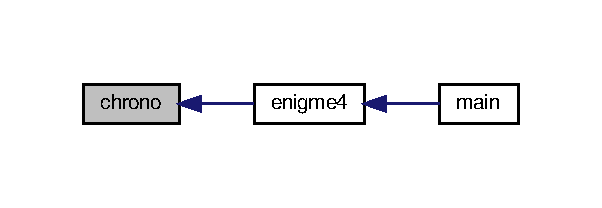
\includegraphics[width=289pt]{enigmes_8c_adc73189bfe920e89bc93d37de8cf28f0_icgraph}
\end{center}
\end{figure}
\mbox{\Hypertarget{enigmes_8c_a07b23a568fbbfcff4c680d4c6af1820a}\label{enigmes_8c_a07b23a568fbbfcff4c680d4c6af1820a}} 
\index{enigmes.\+c@{enigmes.\+c}!enigme1@{enigme1}}
\index{enigme1@{enigme1}!enigmes.\+c@{enigmes.\+c}}
\subsubsection{\texorpdfstring{enigme1()}{enigme1()}}
{\footnotesize\ttfamily int enigme1 (\begin{DoxyParamCaption}\item[{S\+D\+L\+\_\+\+Surface $\ast$}]{screen }\end{DoxyParamCaption})}



pour enigme4 

Here is the caller graph for this function\+:\nopagebreak
\begin{figure}[H]
\begin{center}
\leavevmode
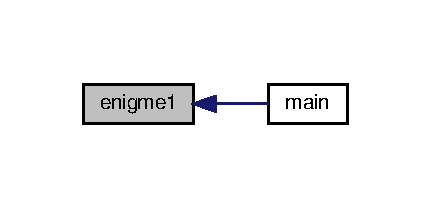
\includegraphics[width=207pt]{enigmes_8c_a07b23a568fbbfcff4c680d4c6af1820a_icgraph}
\end{center}
\end{figure}
\mbox{\Hypertarget{enigmes_8c_ae0f19513f31cfa44736ddefbb15a9a3a}\label{enigmes_8c_ae0f19513f31cfa44736ddefbb15a9a3a}} 
\index{enigmes.\+c@{enigmes.\+c}!enigme2@{enigme2}}
\index{enigme2@{enigme2}!enigmes.\+c@{enigmes.\+c}}
\subsubsection{\texorpdfstring{enigme2()}{enigme2()}}
{\footnotesize\ttfamily int enigme2 (\begin{DoxyParamCaption}\item[{S\+D\+L\+\_\+\+Surface $\ast$}]{screen }\end{DoxyParamCaption})}



enigme 1 math random 

Here is the caller graph for this function\+:\nopagebreak
\begin{figure}[H]
\begin{center}
\leavevmode
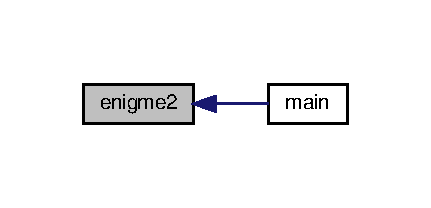
\includegraphics[width=207pt]{enigmes_8c_ae0f19513f31cfa44736ddefbb15a9a3a_icgraph}
\end{center}
\end{figure}
\mbox{\Hypertarget{enigmes_8c_a8dbe78bd6afb9a66a8f8b768bdf7110b}\label{enigmes_8c_a8dbe78bd6afb9a66a8f8b768bdf7110b}} 
\index{enigmes.\+c@{enigmes.\+c}!enigme3@{enigme3}}
\index{enigme3@{enigme3}!enigmes.\+c@{enigmes.\+c}}
\subsubsection{\texorpdfstring{enigme3()}{enigme3()}}
{\footnotesize\ttfamily int enigme3 (\begin{DoxyParamCaption}\item[{S\+D\+L\+\_\+\+Surface $\ast$}]{screen }\end{DoxyParamCaption})}



enigme 2 panda 

Here is the caller graph for this function\+:\nopagebreak
\begin{figure}[H]
\begin{center}
\leavevmode
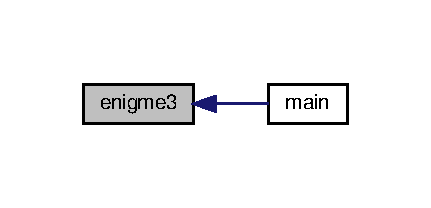
\includegraphics[width=207pt]{enigmes_8c_a8dbe78bd6afb9a66a8f8b768bdf7110b_icgraph}
\end{center}
\end{figure}
\mbox{\Hypertarget{enigmes_8c_a9548e307594e7aa6d2cdbbcbb4156524}\label{enigmes_8c_a9548e307594e7aa6d2cdbbcbb4156524}} 
\index{enigmes.\+c@{enigmes.\+c}!enigme4@{enigme4}}
\index{enigme4@{enigme4}!enigmes.\+c@{enigmes.\+c}}
\subsubsection{\texorpdfstring{enigme4()}{enigme4()}}
{\footnotesize\ttfamily int enigme4 (\begin{DoxyParamCaption}\item[{S\+D\+L\+\_\+\+Surface $\ast$}]{screen }\end{DoxyParamCaption})}



enigme 3 des question apartir d\textquotesingle{}un fichier 

Here is the call graph for this function\+:
\nopagebreak
\begin{figure}[H]
\begin{center}
\leavevmode
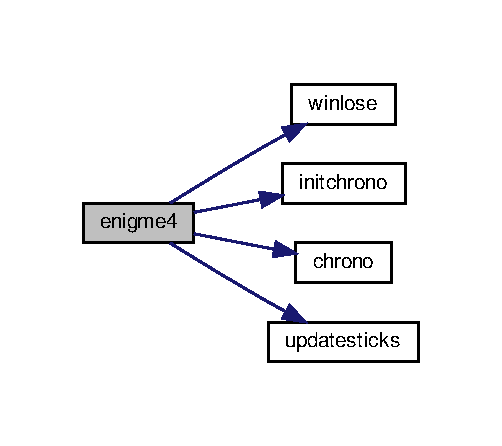
\includegraphics[width=241pt]{enigmes_8c_a9548e307594e7aa6d2cdbbcbb4156524_cgraph}
\end{center}
\end{figure}
Here is the caller graph for this function\+:\nopagebreak
\begin{figure}[H]
\begin{center}
\leavevmode
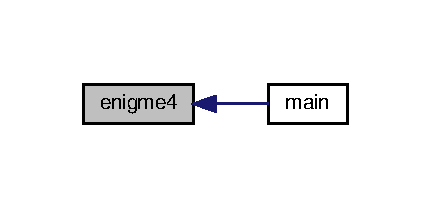
\includegraphics[width=207pt]{enigmes_8c_a9548e307594e7aa6d2cdbbcbb4156524_icgraph}
\end{center}
\end{figure}
\mbox{\Hypertarget{enigmes_8c_a6dd29323933d67965cc4741c9c0b0afa}\label{enigmes_8c_a6dd29323933d67965cc4741c9c0b0afa}} 
\index{enigmes.\+c@{enigmes.\+c}!initchrono@{initchrono}}
\index{initchrono@{initchrono}!enigmes.\+c@{enigmes.\+c}}
\subsubsection{\texorpdfstring{initchrono()}{initchrono()}}
{\footnotesize\ttfamily clock\+\_\+t initchrono (\begin{DoxyParamCaption}\item[{T\+T\+F\+\_\+\+Font $\ast$$\ast$}]{police,  }\item[{S\+D\+L\+\_\+\+Surface $\ast$$\ast$}]{black }\end{DoxyParamCaption})}



resultat enigme 

Here is the caller graph for this function\+:
\nopagebreak
\begin{figure}[H]
\begin{center}
\leavevmode
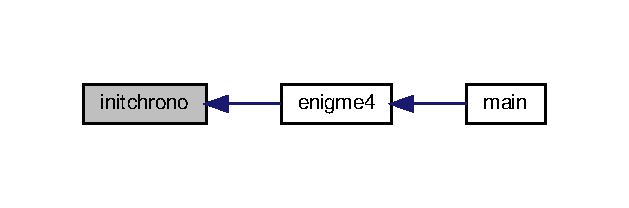
\includegraphics[width=302pt]{enigmes_8c_a6dd29323933d67965cc4741c9c0b0afa_icgraph}
\end{center}
\end{figure}
\mbox{\Hypertarget{enigmes_8c_a6cd927b8211a7ff6445f6dbdeed60413}\label{enigmes_8c_a6cd927b8211a7ff6445f6dbdeed60413}} 
\index{enigmes.\+c@{enigmes.\+c}!resolutionenigme@{resolutionenigme}}
\index{resolutionenigme@{resolutionenigme}!enigmes.\+c@{enigmes.\+c}}
\subsubsection{\texorpdfstring{resolutionenigme()}{resolutionenigme()}}
{\footnotesize\ttfamily int resolutionenigme (\begin{DoxyParamCaption}\item[{int}]{resultat,  }\item[{int}]{resultat2 }\end{DoxyParamCaption})}



affichage enigme 

\mbox{\Hypertarget{enigmes_8c_a3a045cebb7e3097603076d550132c6a5}\label{enigmes_8c_a3a045cebb7e3097603076d550132c6a5}} 
\index{enigmes.\+c@{enigmes.\+c}!updatesticks@{updatesticks}}
\index{updatesticks@{updatesticks}!enigmes.\+c@{enigmes.\+c}}
\subsubsection{\texorpdfstring{updatesticks()}{updatesticks()}}
{\footnotesize\ttfamily int updatesticks (\begin{DoxyParamCaption}\item[{int}]{sticks,  }\item[{S\+D\+L\+\_\+\+Surface $\ast$}]{screen,  }\item[{T\+T\+F\+\_\+\+Font $\ast$}]{police,  }\item[{S\+D\+L\+\_\+\+Surface $\ast$}]{black,  }\item[{int}]{choix }\end{DoxyParamCaption})}



l\textquotesingle{}affichage du chronometre 

Here is the caller graph for this function\+:
\nopagebreak
\begin{figure}[H]
\begin{center}
\leavevmode
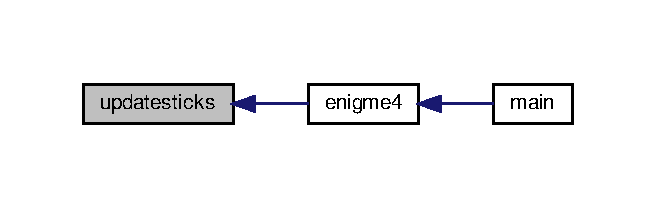
\includegraphics[width=315pt]{enigmes_8c_a3a045cebb7e3097603076d550132c6a5_icgraph}
\end{center}
\end{figure}
\mbox{\Hypertarget{enigmes_8c_acae9a098bc124f835a2f5fd4aecee435}\label{enigmes_8c_acae9a098bc124f835a2f5fd4aecee435}} 
\index{enigmes.\+c@{enigmes.\+c}!winlose@{winlose}}
\index{winlose@{winlose}!enigmes.\+c@{enigmes.\+c}}
\subsubsection{\texorpdfstring{winlose()}{winlose()}}
{\footnotesize\ttfamily int winlose (\begin{DoxyParamCaption}\item[{S\+D\+L\+\_\+\+Surface $\ast$}]{screen,  }\item[{int}]{player,  }\item[{S\+D\+L\+\_\+\+Surface $\ast$}]{win,  }\item[{S\+D\+L\+\_\+\+Surface $\ast$}]{lose,  }\item[{S\+D\+L\+\_\+\+Surface $\ast$}]{rules,  }\item[{S\+D\+L\+\_\+\+Surface $\ast$}]{continu\mbox{[}$\,$\mbox{]},  }\item[{S\+D\+L\+\_\+\+Rect}]{position,  }\item[{int $\ast$}]{lvl }\end{DoxyParamCaption})}



pour l enigme4 

Here is the caller graph for this function\+:
\nopagebreak
\begin{figure}[H]
\begin{center}
\leavevmode
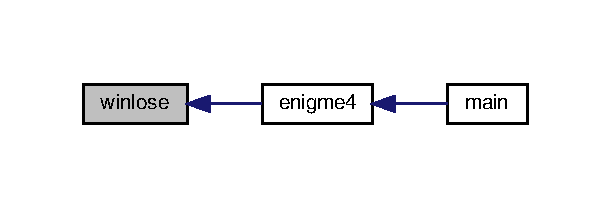
\includegraphics[width=293pt]{enigmes_8c_acae9a098bc124f835a2f5fd4aecee435_icgraph}
\end{center}
\end{figure}

\hypertarget{enigmes_8h}{}\section{enigmes.\+h File Reference}
\label{enigmes_8h}\index{enigmes.\+h@{enigmes.\+h}}


toutes les enigmes  


This graph shows which files directly or indirectly include this file\+:
\nopagebreak
\begin{figure}[H]
\begin{center}
\leavevmode
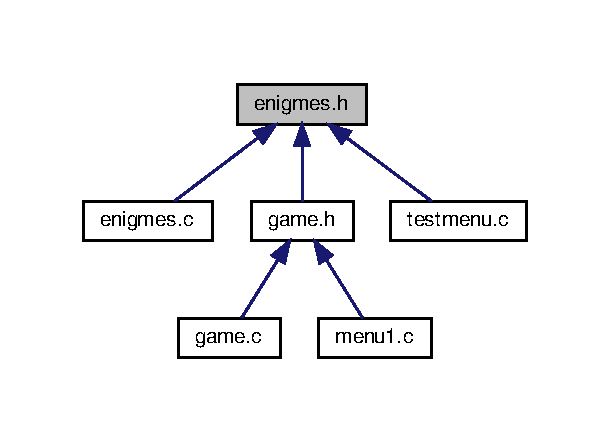
\includegraphics[width=293pt]{enigmes_8h__dep__incl}
\end{center}
\end{figure}
\subsection*{Functions}
\begin{DoxyCompactItemize}
\item 
void \hyperlink{enigmes_8h_abc41653829a3c89b3907cd3ae5927145}{afficherenigme} (S\+D\+L\+\_\+\+Surface $\ast$screen, char $\ast$a)
\item 
int \hyperlink{enigmes_8h_a6cd927b8211a7ff6445f6dbdeed60413}{resolutionenigme} (int resultat, int resultat2)
\begin{DoxyCompactList}\small\item\em affichage enigme \end{DoxyCompactList}\item 
clock\+\_\+t \hyperlink{enigmes_8h_a6dd29323933d67965cc4741c9c0b0afa}{initchrono} (T\+T\+F\+\_\+\+Font $\ast$$\ast$police, S\+D\+L\+\_\+\+Surface $\ast$$\ast$black)
\begin{DoxyCompactList}\small\item\em resultat enigme \end{DoxyCompactList}\item 
int \hyperlink{enigmes_8h_adc73189bfe920e89bc93d37de8cf28f0}{chrono} (clock\+\_\+t debut, S\+D\+L\+\_\+\+Surface $\ast$screen, T\+T\+F\+\_\+\+Font $\ast$police, S\+D\+L\+\_\+\+Surface $\ast$black)
\begin{DoxyCompactList}\small\item\em initialisation du chronometre pour les enigmes \end{DoxyCompactList}\item 
int \hyperlink{enigmes_8h_a3a045cebb7e3097603076d550132c6a5}{updatesticks} (int sticks, S\+D\+L\+\_\+\+Surface $\ast$screen, T\+T\+F\+\_\+\+Font $\ast$police, S\+D\+L\+\_\+\+Surface $\ast$black, int choix)
\begin{DoxyCompactList}\small\item\em l\textquotesingle{}affichage du chronometre \end{DoxyCompactList}\item 
int \hyperlink{enigmes_8h_acae9a098bc124f835a2f5fd4aecee435}{winlose} (S\+D\+L\+\_\+\+Surface $\ast$screen, int player, S\+D\+L\+\_\+\+Surface $\ast$win, S\+D\+L\+\_\+\+Surface $\ast$lose, S\+D\+L\+\_\+\+Surface $\ast$rules, S\+D\+L\+\_\+\+Surface $\ast$continu\mbox{[}$\,$\mbox{]}, S\+D\+L\+\_\+\+Rect position, int $\ast$lvl)
\begin{DoxyCompactList}\small\item\em pour l enigme4 \end{DoxyCompactList}\item 
int \hyperlink{enigmes_8h_a07b23a568fbbfcff4c680d4c6af1820a}{enigme1} (S\+D\+L\+\_\+\+Surface $\ast$screen)
\begin{DoxyCompactList}\small\item\em pour enigme4 \end{DoxyCompactList}\item 
int \hyperlink{enigmes_8h_ae0f19513f31cfa44736ddefbb15a9a3a}{enigme2} (S\+D\+L\+\_\+\+Surface $\ast$screen)
\begin{DoxyCompactList}\small\item\em enigme 1 math random \end{DoxyCompactList}\item 
int \hyperlink{enigmes_8h_a8dbe78bd6afb9a66a8f8b768bdf7110b}{enigme3} (S\+D\+L\+\_\+\+Surface $\ast$screen)
\begin{DoxyCompactList}\small\item\em enigme 2 panda \end{DoxyCompactList}\item 
int \hyperlink{enigmes_8h_a9548e307594e7aa6d2cdbbcbb4156524}{enigme4} (S\+D\+L\+\_\+\+Surface $\ast$screen)
\begin{DoxyCompactList}\small\item\em enigme 3 des question apartir d\textquotesingle{}un fichier \end{DoxyCompactList}\end{DoxyCompactItemize}


\subsection{Detailed Description}
toutes les enigmes 

\begin{DoxyAuthor}{Author}
Mohamed Ali Bouzaiene 
\end{DoxyAuthor}
\begin{DoxyVersion}{Version}
0.\+0.\+1 
\end{DoxyVersion}


\subsection{Function Documentation}
\mbox{\Hypertarget{enigmes_8h_abc41653829a3c89b3907cd3ae5927145}\label{enigmes_8h_abc41653829a3c89b3907cd3ae5927145}} 
\index{enigmes.\+h@{enigmes.\+h}!afficherenigme@{afficherenigme}}
\index{afficherenigme@{afficherenigme}!enigmes.\+h@{enigmes.\+h}}
\subsubsection{\texorpdfstring{afficherenigme()}{afficherenigme()}}
{\footnotesize\ttfamily void afficherenigme (\begin{DoxyParamCaption}\item[{S\+D\+L\+\_\+\+Surface $\ast$}]{screen,  }\item[{char $\ast$}]{a }\end{DoxyParamCaption})}

\mbox{\Hypertarget{enigmes_8h_adc73189bfe920e89bc93d37de8cf28f0}\label{enigmes_8h_adc73189bfe920e89bc93d37de8cf28f0}} 
\index{enigmes.\+h@{enigmes.\+h}!chrono@{chrono}}
\index{chrono@{chrono}!enigmes.\+h@{enigmes.\+h}}
\subsubsection{\texorpdfstring{chrono()}{chrono()}}
{\footnotesize\ttfamily int chrono (\begin{DoxyParamCaption}\item[{clock\+\_\+t}]{debut,  }\item[{S\+D\+L\+\_\+\+Surface $\ast$}]{screen,  }\item[{T\+T\+F\+\_\+\+Font $\ast$}]{police,  }\item[{S\+D\+L\+\_\+\+Surface $\ast$}]{black }\end{DoxyParamCaption})}



initialisation du chronometre pour les enigmes 

Here is the caller graph for this function\+:
\nopagebreak
\begin{figure}[H]
\begin{center}
\leavevmode
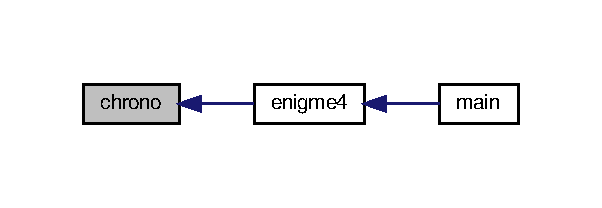
\includegraphics[width=289pt]{enigmes_8h_adc73189bfe920e89bc93d37de8cf28f0_icgraph}
\end{center}
\end{figure}
\mbox{\Hypertarget{enigmes_8h_a07b23a568fbbfcff4c680d4c6af1820a}\label{enigmes_8h_a07b23a568fbbfcff4c680d4c6af1820a}} 
\index{enigmes.\+h@{enigmes.\+h}!enigme1@{enigme1}}
\index{enigme1@{enigme1}!enigmes.\+h@{enigmes.\+h}}
\subsubsection{\texorpdfstring{enigme1()}{enigme1()}}
{\footnotesize\ttfamily int enigme1 (\begin{DoxyParamCaption}\item[{S\+D\+L\+\_\+\+Surface $\ast$}]{screen }\end{DoxyParamCaption})}



pour enigme4 

Here is the caller graph for this function\+:\nopagebreak
\begin{figure}[H]
\begin{center}
\leavevmode
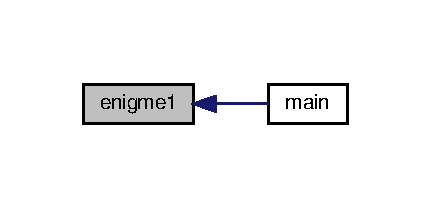
\includegraphics[width=207pt]{enigmes_8h_a07b23a568fbbfcff4c680d4c6af1820a_icgraph}
\end{center}
\end{figure}
\mbox{\Hypertarget{enigmes_8h_ae0f19513f31cfa44736ddefbb15a9a3a}\label{enigmes_8h_ae0f19513f31cfa44736ddefbb15a9a3a}} 
\index{enigmes.\+h@{enigmes.\+h}!enigme2@{enigme2}}
\index{enigme2@{enigme2}!enigmes.\+h@{enigmes.\+h}}
\subsubsection{\texorpdfstring{enigme2()}{enigme2()}}
{\footnotesize\ttfamily int enigme2 (\begin{DoxyParamCaption}\item[{S\+D\+L\+\_\+\+Surface $\ast$}]{screen }\end{DoxyParamCaption})}



enigme 1 math random 

Here is the caller graph for this function\+:\nopagebreak
\begin{figure}[H]
\begin{center}
\leavevmode
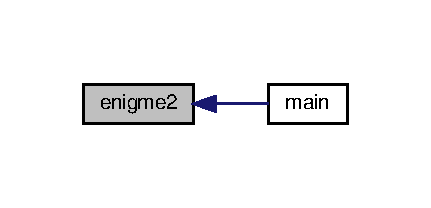
\includegraphics[width=207pt]{enigmes_8h_ae0f19513f31cfa44736ddefbb15a9a3a_icgraph}
\end{center}
\end{figure}
\mbox{\Hypertarget{enigmes_8h_a8dbe78bd6afb9a66a8f8b768bdf7110b}\label{enigmes_8h_a8dbe78bd6afb9a66a8f8b768bdf7110b}} 
\index{enigmes.\+h@{enigmes.\+h}!enigme3@{enigme3}}
\index{enigme3@{enigme3}!enigmes.\+h@{enigmes.\+h}}
\subsubsection{\texorpdfstring{enigme3()}{enigme3()}}
{\footnotesize\ttfamily int enigme3 (\begin{DoxyParamCaption}\item[{S\+D\+L\+\_\+\+Surface $\ast$}]{screen }\end{DoxyParamCaption})}



enigme 2 panda 

Here is the caller graph for this function\+:\nopagebreak
\begin{figure}[H]
\begin{center}
\leavevmode
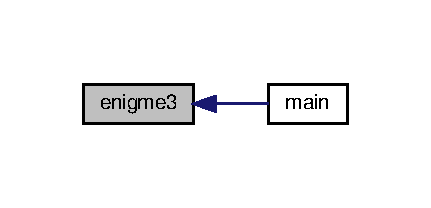
\includegraphics[width=207pt]{enigmes_8h_a8dbe78bd6afb9a66a8f8b768bdf7110b_icgraph}
\end{center}
\end{figure}
\mbox{\Hypertarget{enigmes_8h_a9548e307594e7aa6d2cdbbcbb4156524}\label{enigmes_8h_a9548e307594e7aa6d2cdbbcbb4156524}} 
\index{enigmes.\+h@{enigmes.\+h}!enigme4@{enigme4}}
\index{enigme4@{enigme4}!enigmes.\+h@{enigmes.\+h}}
\subsubsection{\texorpdfstring{enigme4()}{enigme4()}}
{\footnotesize\ttfamily int enigme4 (\begin{DoxyParamCaption}\item[{S\+D\+L\+\_\+\+Surface $\ast$}]{screen }\end{DoxyParamCaption})}



enigme 3 des question apartir d\textquotesingle{}un fichier 

Here is the call graph for this function\+:
\nopagebreak
\begin{figure}[H]
\begin{center}
\leavevmode
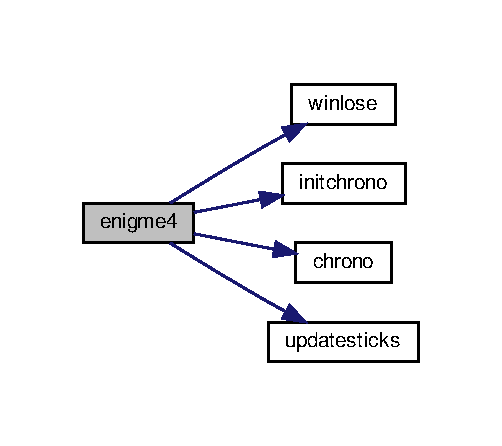
\includegraphics[width=241pt]{enigmes_8h_a9548e307594e7aa6d2cdbbcbb4156524_cgraph}
\end{center}
\end{figure}
Here is the caller graph for this function\+:\nopagebreak
\begin{figure}[H]
\begin{center}
\leavevmode
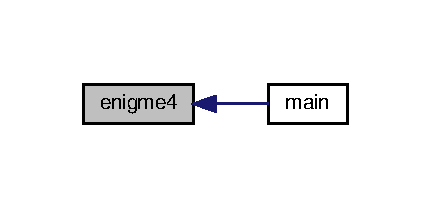
\includegraphics[width=207pt]{enigmes_8h_a9548e307594e7aa6d2cdbbcbb4156524_icgraph}
\end{center}
\end{figure}
\mbox{\Hypertarget{enigmes_8h_a6dd29323933d67965cc4741c9c0b0afa}\label{enigmes_8h_a6dd29323933d67965cc4741c9c0b0afa}} 
\index{enigmes.\+h@{enigmes.\+h}!initchrono@{initchrono}}
\index{initchrono@{initchrono}!enigmes.\+h@{enigmes.\+h}}
\subsubsection{\texorpdfstring{initchrono()}{initchrono()}}
{\footnotesize\ttfamily clock\+\_\+t initchrono (\begin{DoxyParamCaption}\item[{T\+T\+F\+\_\+\+Font $\ast$$\ast$}]{police,  }\item[{S\+D\+L\+\_\+\+Surface $\ast$$\ast$}]{black }\end{DoxyParamCaption})}



resultat enigme 

Here is the caller graph for this function\+:
\nopagebreak
\begin{figure}[H]
\begin{center}
\leavevmode
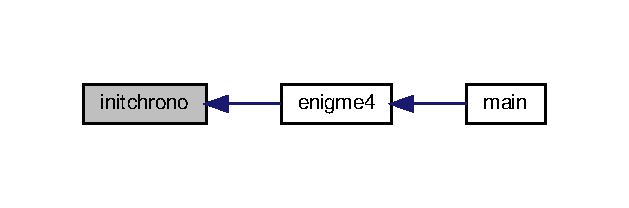
\includegraphics[width=302pt]{enigmes_8h_a6dd29323933d67965cc4741c9c0b0afa_icgraph}
\end{center}
\end{figure}
\mbox{\Hypertarget{enigmes_8h_a6cd927b8211a7ff6445f6dbdeed60413}\label{enigmes_8h_a6cd927b8211a7ff6445f6dbdeed60413}} 
\index{enigmes.\+h@{enigmes.\+h}!resolutionenigme@{resolutionenigme}}
\index{resolutionenigme@{resolutionenigme}!enigmes.\+h@{enigmes.\+h}}
\subsubsection{\texorpdfstring{resolutionenigme()}{resolutionenigme()}}
{\footnotesize\ttfamily int resolutionenigme (\begin{DoxyParamCaption}\item[{int}]{resultat,  }\item[{int}]{resultat2 }\end{DoxyParamCaption})}



affichage enigme 

\mbox{\Hypertarget{enigmes_8h_a3a045cebb7e3097603076d550132c6a5}\label{enigmes_8h_a3a045cebb7e3097603076d550132c6a5}} 
\index{enigmes.\+h@{enigmes.\+h}!updatesticks@{updatesticks}}
\index{updatesticks@{updatesticks}!enigmes.\+h@{enigmes.\+h}}
\subsubsection{\texorpdfstring{updatesticks()}{updatesticks()}}
{\footnotesize\ttfamily int updatesticks (\begin{DoxyParamCaption}\item[{int}]{sticks,  }\item[{S\+D\+L\+\_\+\+Surface $\ast$}]{screen,  }\item[{T\+T\+F\+\_\+\+Font $\ast$}]{police,  }\item[{S\+D\+L\+\_\+\+Surface $\ast$}]{black,  }\item[{int}]{choix }\end{DoxyParamCaption})}



l\textquotesingle{}affichage du chronometre 

Here is the caller graph for this function\+:
\nopagebreak
\begin{figure}[H]
\begin{center}
\leavevmode
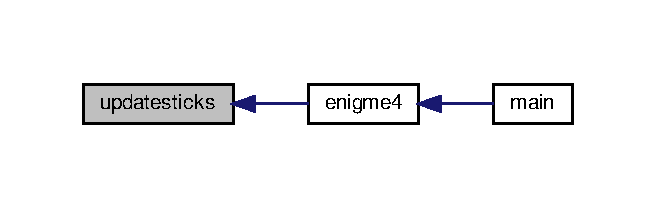
\includegraphics[width=315pt]{enigmes_8h_a3a045cebb7e3097603076d550132c6a5_icgraph}
\end{center}
\end{figure}
\mbox{\Hypertarget{enigmes_8h_acae9a098bc124f835a2f5fd4aecee435}\label{enigmes_8h_acae9a098bc124f835a2f5fd4aecee435}} 
\index{enigmes.\+h@{enigmes.\+h}!winlose@{winlose}}
\index{winlose@{winlose}!enigmes.\+h@{enigmes.\+h}}
\subsubsection{\texorpdfstring{winlose()}{winlose()}}
{\footnotesize\ttfamily int winlose (\begin{DoxyParamCaption}\item[{S\+D\+L\+\_\+\+Surface $\ast$}]{screen,  }\item[{int}]{player,  }\item[{S\+D\+L\+\_\+\+Surface $\ast$}]{win,  }\item[{S\+D\+L\+\_\+\+Surface $\ast$}]{lose,  }\item[{S\+D\+L\+\_\+\+Surface $\ast$}]{rules,  }\item[{S\+D\+L\+\_\+\+Surface $\ast$}]{continu\mbox{[}$\,$\mbox{]},  }\item[{S\+D\+L\+\_\+\+Rect}]{position,  }\item[{int $\ast$}]{lvl }\end{DoxyParamCaption})}



pour l enigme4 

Here is the caller graph for this function\+:
\nopagebreak
\begin{figure}[H]
\begin{center}
\leavevmode
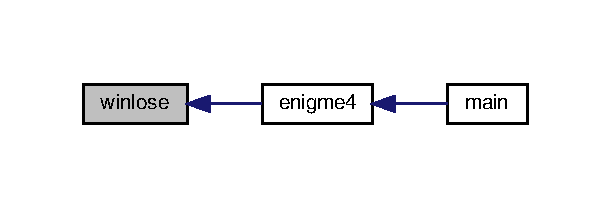
\includegraphics[width=293pt]{enigmes_8h_acae9a098bc124f835a2f5fd4aecee435_icgraph}
\end{center}
\end{figure}

\hypertarget{ennemy_8c}{}\section{ennemy.\+c File Reference}
\label{ennemy_8c}\index{ennemy.\+c@{ennemy.\+c}}
{\ttfamily \#include \char`\"{}ennemy.\+h\char`\"{}}\newline
Include dependency graph for ennemy.\+c\+:\nopagebreak
\begin{figure}[H]
\begin{center}
\leavevmode
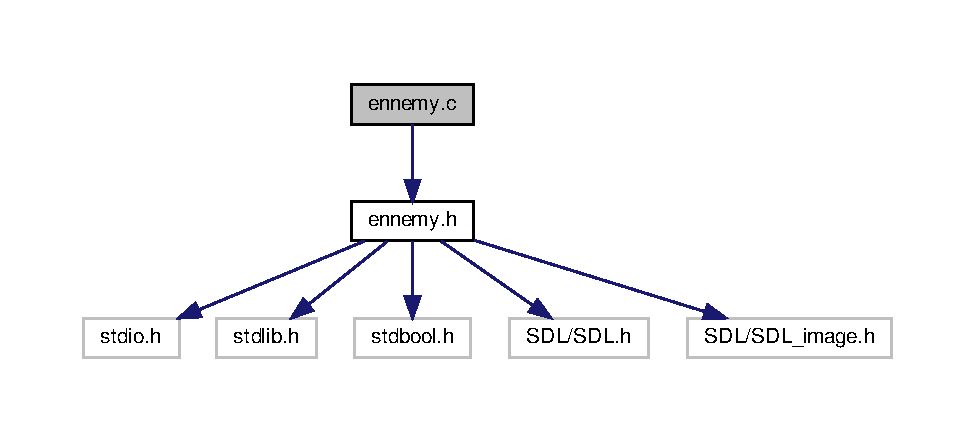
\includegraphics[width=350pt]{ennemy_8c__incl}
\end{center}
\end{figure}
\subsection*{Functions}
\begin{DoxyCompactItemize}
\item 
void \hyperlink{ennemy_8c_aa58979863ea659226f334d656563cc31}{Initialisation\+\_\+\+Ennemy} (\hyperlink{structEnnemy}{Ennemy} $\ast$e, S\+D\+L\+\_\+\+Rect pos)
\item 
void \hyperlink{ennemy_8c_a2841f886f4e83d47d29070d439de66f7}{Display\+\_\+\+Ennemy} (\hyperlink{structEnnemy}{Ennemy} $\ast$e, S\+D\+L\+\_\+\+Surface $\ast$ecran, S\+D\+L\+\_\+\+Rect pos)
\item 
void \hyperlink{ennemy_8c_aef30f17c3373b11470ea17de0daf4fb5}{Animation\+\_\+\+Ennemy} (\hyperlink{structEnnemy}{Ennemy} $\ast$e)
\item 
void \hyperlink{ennemy_8c_a35f3a663d7b93ce02ae0fc5069795fd0}{Free\+\_\+\+Ennemy} (\hyperlink{structEnnemy}{Ennemy} $\ast$e)
\end{DoxyCompactItemize}


\subsection{Function Documentation}
\mbox{\Hypertarget{ennemy_8c_aef30f17c3373b11470ea17de0daf4fb5}\label{ennemy_8c_aef30f17c3373b11470ea17de0daf4fb5}} 
\index{ennemy.\+c@{ennemy.\+c}!Animation\+\_\+\+Ennemy@{Animation\+\_\+\+Ennemy}}
\index{Animation\+\_\+\+Ennemy@{Animation\+\_\+\+Ennemy}!ennemy.\+c@{ennemy.\+c}}
\subsubsection{\texorpdfstring{Animation\+\_\+\+Ennemy()}{Animation\_Ennemy()}}
{\footnotesize\ttfamily void Animation\+\_\+\+Ennemy (\begin{DoxyParamCaption}\item[{\hyperlink{structEnnemy}{Ennemy} $\ast$}]{e }\end{DoxyParamCaption})}

Here is the caller graph for this function\+:\nopagebreak
\begin{figure}[H]
\begin{center}
\leavevmode
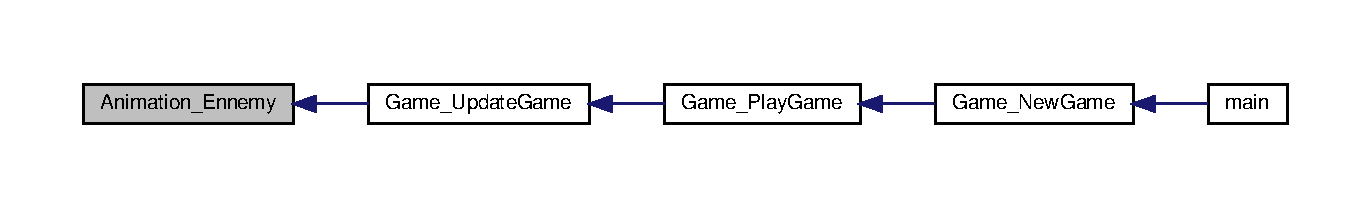
\includegraphics[width=350pt]{ennemy_8c_aef30f17c3373b11470ea17de0daf4fb5_icgraph}
\end{center}
\end{figure}
\mbox{\Hypertarget{ennemy_8c_a2841f886f4e83d47d29070d439de66f7}\label{ennemy_8c_a2841f886f4e83d47d29070d439de66f7}} 
\index{ennemy.\+c@{ennemy.\+c}!Display\+\_\+\+Ennemy@{Display\+\_\+\+Ennemy}}
\index{Display\+\_\+\+Ennemy@{Display\+\_\+\+Ennemy}!ennemy.\+c@{ennemy.\+c}}
\subsubsection{\texorpdfstring{Display\+\_\+\+Ennemy()}{Display\_Ennemy()}}
{\footnotesize\ttfamily void Display\+\_\+\+Ennemy (\begin{DoxyParamCaption}\item[{\hyperlink{structEnnemy}{Ennemy} $\ast$}]{e,  }\item[{S\+D\+L\+\_\+\+Surface $\ast$}]{ecran,  }\item[{S\+D\+L\+\_\+\+Rect}]{pos }\end{DoxyParamCaption})}

Here is the caller graph for this function\+:\nopagebreak
\begin{figure}[H]
\begin{center}
\leavevmode
\includegraphics[width=350pt]{ennemy_8c_a2841f886f4e83d47d29070d439de66f7_icgraph}
\end{center}
\end{figure}
\mbox{\Hypertarget{ennemy_8c_a35f3a663d7b93ce02ae0fc5069795fd0}\label{ennemy_8c_a35f3a663d7b93ce02ae0fc5069795fd0}} 
\index{ennemy.\+c@{ennemy.\+c}!Free\+\_\+\+Ennemy@{Free\+\_\+\+Ennemy}}
\index{Free\+\_\+\+Ennemy@{Free\+\_\+\+Ennemy}!ennemy.\+c@{ennemy.\+c}}
\subsubsection{\texorpdfstring{Free\+\_\+\+Ennemy()}{Free\_Ennemy()}}
{\footnotesize\ttfamily void Free\+\_\+\+Ennemy (\begin{DoxyParamCaption}\item[{\hyperlink{structEnnemy}{Ennemy} $\ast$}]{e }\end{DoxyParamCaption})}

Here is the caller graph for this function\+:\nopagebreak
\begin{figure}[H]
\begin{center}
\leavevmode
\includegraphics[width=350pt]{ennemy_8c_a35f3a663d7b93ce02ae0fc5069795fd0_icgraph}
\end{center}
\end{figure}
\mbox{\Hypertarget{ennemy_8c_aa58979863ea659226f334d656563cc31}\label{ennemy_8c_aa58979863ea659226f334d656563cc31}} 
\index{ennemy.\+c@{ennemy.\+c}!Initialisation\+\_\+\+Ennemy@{Initialisation\+\_\+\+Ennemy}}
\index{Initialisation\+\_\+\+Ennemy@{Initialisation\+\_\+\+Ennemy}!ennemy.\+c@{ennemy.\+c}}
\subsubsection{\texorpdfstring{Initialisation\+\_\+\+Ennemy()}{Initialisation\_Ennemy()}}
{\footnotesize\ttfamily void Initialisation\+\_\+\+Ennemy (\begin{DoxyParamCaption}\item[{\hyperlink{structEnnemy}{Ennemy} $\ast$}]{e,  }\item[{S\+D\+L\+\_\+\+Rect}]{pos }\end{DoxyParamCaption})}

Here is the caller graph for this function\+:\nopagebreak
\begin{figure}[H]
\begin{center}
\leavevmode
\includegraphics[width=350pt]{ennemy_8c_aa58979863ea659226f334d656563cc31_icgraph}
\end{center}
\end{figure}

\hypertarget{ennemy_8h}{}\section{ennemy.\+h File Reference}
\label{ennemy_8h}\index{ennemy.\+h@{ennemy.\+h}}
{\ttfamily \#include $<$stdio.\+h$>$}\newline
{\ttfamily \#include $<$stdlib.\+h$>$}\newline
{\ttfamily \#include $<$stdbool.\+h$>$}\newline
{\ttfamily \#include $<$S\+D\+L/\+S\+D\+L.\+h$>$}\newline
{\ttfamily \#include $<$S\+D\+L/\+S\+D\+L\+\_\+image.\+h$>$}\newline
Include dependency graph for ennemy.\+h\+:\nopagebreak
\begin{figure}[H]
\begin{center}
\leavevmode
\includegraphics[width=350pt]{ennemy_8h__incl}
\end{center}
\end{figure}
This graph shows which files directly or indirectly include this file\+:\nopagebreak
\begin{figure}[H]
\begin{center}
\leavevmode
\includegraphics[width=244pt]{ennemy_8h__dep__incl}
\end{center}
\end{figure}
\subsection*{Data Structures}
\begin{DoxyCompactItemize}
\item 
struct \hyperlink{structEnnemy}{Ennemy}
\end{DoxyCompactItemize}
\subsection*{Functions}
\begin{DoxyCompactItemize}
\item 
void \hyperlink{ennemy_8h_aa58979863ea659226f334d656563cc31}{Initialisation\+\_\+\+Ennemy} (\hyperlink{structEnnemy}{Ennemy} $\ast$e, S\+D\+L\+\_\+\+Rect pos)
\item 
void \hyperlink{ennemy_8h_a2841f886f4e83d47d29070d439de66f7}{Display\+\_\+\+Ennemy} (\hyperlink{structEnnemy}{Ennemy} $\ast$e, S\+D\+L\+\_\+\+Surface $\ast$ecran, S\+D\+L\+\_\+\+Rect pos)
\item 
void \hyperlink{ennemy_8h_aef30f17c3373b11470ea17de0daf4fb5}{Animation\+\_\+\+Ennemy} (\hyperlink{structEnnemy}{Ennemy} $\ast$e)
\item 
void \hyperlink{ennemy_8h_a35f3a663d7b93ce02ae0fc5069795fd0}{Free\+\_\+\+Ennemy} (\hyperlink{structEnnemy}{Ennemy} $\ast$e)
\end{DoxyCompactItemize}


\subsection{Function Documentation}
\mbox{\Hypertarget{ennemy_8h_aef30f17c3373b11470ea17de0daf4fb5}\label{ennemy_8h_aef30f17c3373b11470ea17de0daf4fb5}} 
\index{ennemy.\+h@{ennemy.\+h}!Animation\+\_\+\+Ennemy@{Animation\+\_\+\+Ennemy}}
\index{Animation\+\_\+\+Ennemy@{Animation\+\_\+\+Ennemy}!ennemy.\+h@{ennemy.\+h}}
\subsubsection{\texorpdfstring{Animation\+\_\+\+Ennemy()}{Animation\_Ennemy()}}
{\footnotesize\ttfamily void Animation\+\_\+\+Ennemy (\begin{DoxyParamCaption}\item[{\hyperlink{structEnnemy}{Ennemy} $\ast$}]{e }\end{DoxyParamCaption})}

Here is the caller graph for this function\+:\nopagebreak
\begin{figure}[H]
\begin{center}
\leavevmode
\includegraphics[width=350pt]{ennemy_8h_aef30f17c3373b11470ea17de0daf4fb5_icgraph}
\end{center}
\end{figure}
\mbox{\Hypertarget{ennemy_8h_a2841f886f4e83d47d29070d439de66f7}\label{ennemy_8h_a2841f886f4e83d47d29070d439de66f7}} 
\index{ennemy.\+h@{ennemy.\+h}!Display\+\_\+\+Ennemy@{Display\+\_\+\+Ennemy}}
\index{Display\+\_\+\+Ennemy@{Display\+\_\+\+Ennemy}!ennemy.\+h@{ennemy.\+h}}
\subsubsection{\texorpdfstring{Display\+\_\+\+Ennemy()}{Display\_Ennemy()}}
{\footnotesize\ttfamily void Display\+\_\+\+Ennemy (\begin{DoxyParamCaption}\item[{\hyperlink{structEnnemy}{Ennemy} $\ast$}]{e,  }\item[{S\+D\+L\+\_\+\+Surface $\ast$}]{ecran,  }\item[{S\+D\+L\+\_\+\+Rect}]{pos }\end{DoxyParamCaption})}

Here is the caller graph for this function\+:\nopagebreak
\begin{figure}[H]
\begin{center}
\leavevmode
\includegraphics[width=350pt]{ennemy_8h_a2841f886f4e83d47d29070d439de66f7_icgraph}
\end{center}
\end{figure}
\mbox{\Hypertarget{ennemy_8h_a35f3a663d7b93ce02ae0fc5069795fd0}\label{ennemy_8h_a35f3a663d7b93ce02ae0fc5069795fd0}} 
\index{ennemy.\+h@{ennemy.\+h}!Free\+\_\+\+Ennemy@{Free\+\_\+\+Ennemy}}
\index{Free\+\_\+\+Ennemy@{Free\+\_\+\+Ennemy}!ennemy.\+h@{ennemy.\+h}}
\subsubsection{\texorpdfstring{Free\+\_\+\+Ennemy()}{Free\_Ennemy()}}
{\footnotesize\ttfamily void Free\+\_\+\+Ennemy (\begin{DoxyParamCaption}\item[{\hyperlink{structEnnemy}{Ennemy} $\ast$}]{e }\end{DoxyParamCaption})}

Here is the caller graph for this function\+:\nopagebreak
\begin{figure}[H]
\begin{center}
\leavevmode
\includegraphics[width=350pt]{ennemy_8h_a35f3a663d7b93ce02ae0fc5069795fd0_icgraph}
\end{center}
\end{figure}
\mbox{\Hypertarget{ennemy_8h_aa58979863ea659226f334d656563cc31}\label{ennemy_8h_aa58979863ea659226f334d656563cc31}} 
\index{ennemy.\+h@{ennemy.\+h}!Initialisation\+\_\+\+Ennemy@{Initialisation\+\_\+\+Ennemy}}
\index{Initialisation\+\_\+\+Ennemy@{Initialisation\+\_\+\+Ennemy}!ennemy.\+h@{ennemy.\+h}}
\subsubsection{\texorpdfstring{Initialisation\+\_\+\+Ennemy()}{Initialisation\_Ennemy()}}
{\footnotesize\ttfamily void Initialisation\+\_\+\+Ennemy (\begin{DoxyParamCaption}\item[{\hyperlink{structEnnemy}{Ennemy} $\ast$}]{e,  }\item[{S\+D\+L\+\_\+\+Rect}]{pos }\end{DoxyParamCaption})}

Here is the caller graph for this function\+:\nopagebreak
\begin{figure}[H]
\begin{center}
\leavevmode
\includegraphics[width=350pt]{ennemy_8h_aa58979863ea659226f334d656563cc31_icgraph}
\end{center}
\end{figure}

\hypertarget{fonctions_8c}{}\section{fonctions.\+c File Reference}
\label{fonctions_8c}\index{fonctions.\+c@{fonctions.\+c}}


all the menu functions  


{\ttfamily \#include $<$stdlib.\+h$>$}\newline
{\ttfamily \#include $<$stdio.\+h$>$}\newline
{\ttfamily \#include $<$S\+D\+L/\+S\+D\+L.\+h$>$}\newline
{\ttfamily \#include $<$S\+D\+L/\+S\+D\+L\+\_\+ttf.\+h$>$}\newline
{\ttfamily \#include $<$S\+D\+L/\+S\+D\+L\+\_\+image.\+h$>$}\newline
{\ttfamily \#include $<$S\+D\+L/\+S\+D\+L\+\_\+mixer.\+h$>$}\newline
{\ttfamily \#include \char`\"{}fonctions.\+h\char`\"{}}\newline
Include dependency graph for fonctions.\+c\+:\nopagebreak
\begin{figure}[H]
\begin{center}
\leavevmode
\includegraphics[width=350pt]{fonctions_8c__incl}
\end{center}
\end{figure}
\subsection*{Functions}
\begin{DoxyCompactItemize}
\item 
void \hyperlink{fonctions_8c_af0310f8c3d32415e9abfbe927a27774a}{menu} (S\+D\+L\+\_\+\+Surface $\ast$background, S\+D\+L\+\_\+\+Surface $\ast$screen, S\+D\+L\+\_\+\+Rect positionbackground, \hyperlink{structtexte}{texte} $\ast$txt, S\+D\+L\+\_\+\+Surface $\ast$play, S\+D\+L\+\_\+\+Surface $\ast$setting, S\+D\+L\+\_\+\+Surface $\ast$quit, S\+D\+L\+\_\+\+Rect positionplay, S\+D\+L\+\_\+\+Rect positionsetting, S\+D\+L\+\_\+\+Rect positionquit, S\+D\+L\+\_\+\+Surface $\ast$credits, S\+D\+L\+\_\+\+Rect positioncredits)
\item 
void \hyperlink{fonctions_8c_a7aa52168ae5dc669d191ac754416de1d}{menu1} (S\+D\+L\+\_\+\+Surface $\ast$background1, S\+D\+L\+\_\+\+Surface $\ast$screen, S\+D\+L\+\_\+\+Rect positionbackground)
\item 
void \hyperlink{fonctions_8c_ad6658c6ffe84f3432b1440fd7168e81a}{fleche} (int etat, S\+D\+L\+\_\+\+Surface $\ast$screen, S\+D\+L\+\_\+\+Surface $\ast$play, S\+D\+L\+\_\+\+Surface $\ast$quit, S\+D\+L\+\_\+\+Surface $\ast$setting, S\+D\+L\+\_\+\+Surface $\ast$credits, S\+D\+L\+\_\+\+Surface $\ast$quit1, S\+D\+L\+\_\+\+Surface $\ast$setting1, S\+D\+L\+\_\+\+Surface $\ast$play1, S\+D\+L\+\_\+\+Surface $\ast$credits1, S\+D\+L\+\_\+\+Rect positionplay, S\+D\+L\+\_\+\+Rect positionquit, S\+D\+L\+\_\+\+Rect positionsetting, S\+D\+L\+\_\+\+Rect positioncredits)
\begin{DoxyCompactList}\small\item\em to show the menu \end{DoxyCompactList}\item 
void \hyperlink{fonctions_8c_a79360bb9b1585cfa4f57b551335491c2}{animation1} (S\+D\+L\+\_\+\+Surface $\ast$background3, S\+D\+L\+\_\+\+Surface $\ast$screen, S\+D\+L\+\_\+\+Rect $\ast$position, S\+D\+L\+\_\+\+Surface $\ast$background1, S\+D\+L\+\_\+\+Rect positionbackground)
\begin{DoxyCompactList}\small\item\em to move with the arrows on the menu \end{DoxyCompactList}\item 
int \hyperlink{fonctions_8c_a1e0d526d92db41be5f0c1609a1071e61}{personnage} (S\+D\+L\+\_\+\+Surface $\ast$screen)
\begin{DoxyCompactList}\small\item\em to animate the background \end{DoxyCompactList}\item 
int \hyperlink{fonctions_8c_a4840e5a896d43999cfcf0fb32acbd13d}{change} (S\+D\+L\+\_\+\+Surface $\ast$screen)
\begin{DoxyCompactList}\small\item\em to change the player \end{DoxyCompactList}\end{DoxyCompactItemize}


\subsection{Detailed Description}
all the menu functions 

\begin{DoxyAuthor}{Author}
Mohamed Ali Bouzaiene 
\end{DoxyAuthor}
\begin{DoxyVersion}{Version}
0.\+0.\+1 
\end{DoxyVersion}


\subsection{Function Documentation}
\mbox{\Hypertarget{fonctions_8c_a79360bb9b1585cfa4f57b551335491c2}\label{fonctions_8c_a79360bb9b1585cfa4f57b551335491c2}} 
\index{fonctions.\+c@{fonctions.\+c}!animation1@{animation1}}
\index{animation1@{animation1}!fonctions.\+c@{fonctions.\+c}}
\subsubsection{\texorpdfstring{animation1()}{animation1()}}
{\footnotesize\ttfamily void animation1 (\begin{DoxyParamCaption}\item[{S\+D\+L\+\_\+\+Surface $\ast$}]{background3,  }\item[{S\+D\+L\+\_\+\+Surface $\ast$}]{screen,  }\item[{S\+D\+L\+\_\+\+Rect $\ast$}]{position,  }\item[{S\+D\+L\+\_\+\+Surface $\ast$}]{background1,  }\item[{S\+D\+L\+\_\+\+Rect}]{positionbackground }\end{DoxyParamCaption})}



to move with the arrows on the menu 

Here is the caller graph for this function\+:\nopagebreak
\begin{figure}[H]
\begin{center}
\leavevmode
\includegraphics[width=218pt]{fonctions_8c_a79360bb9b1585cfa4f57b551335491c2_icgraph}
\end{center}
\end{figure}
\mbox{\Hypertarget{fonctions_8c_a4840e5a896d43999cfcf0fb32acbd13d}\label{fonctions_8c_a4840e5a896d43999cfcf0fb32acbd13d}} 
\index{fonctions.\+c@{fonctions.\+c}!change@{change}}
\index{change@{change}!fonctions.\+c@{fonctions.\+c}}
\subsubsection{\texorpdfstring{change()}{change()}}
{\footnotesize\ttfamily int change (\begin{DoxyParamCaption}\item[{S\+D\+L\+\_\+\+Surface $\ast$}]{screen }\end{DoxyParamCaption})}



to change the player 

Here is the caller graph for this function\+:\nopagebreak
\begin{figure}[H]
\begin{center}
\leavevmode
\includegraphics[width=202pt]{fonctions_8c_a4840e5a896d43999cfcf0fb32acbd13d_icgraph}
\end{center}
\end{figure}
\mbox{\Hypertarget{fonctions_8c_ad6658c6ffe84f3432b1440fd7168e81a}\label{fonctions_8c_ad6658c6ffe84f3432b1440fd7168e81a}} 
\index{fonctions.\+c@{fonctions.\+c}!fleche@{fleche}}
\index{fleche@{fleche}!fonctions.\+c@{fonctions.\+c}}
\subsubsection{\texorpdfstring{fleche()}{fleche()}}
{\footnotesize\ttfamily void fleche (\begin{DoxyParamCaption}\item[{int}]{etat,  }\item[{S\+D\+L\+\_\+\+Surface $\ast$}]{screen,  }\item[{S\+D\+L\+\_\+\+Surface $\ast$}]{play,  }\item[{S\+D\+L\+\_\+\+Surface $\ast$}]{quit,  }\item[{S\+D\+L\+\_\+\+Surface $\ast$}]{setting,  }\item[{S\+D\+L\+\_\+\+Surface $\ast$}]{credits,  }\item[{S\+D\+L\+\_\+\+Surface $\ast$}]{quit1,  }\item[{S\+D\+L\+\_\+\+Surface $\ast$}]{setting1,  }\item[{S\+D\+L\+\_\+\+Surface $\ast$}]{play1,  }\item[{S\+D\+L\+\_\+\+Surface $\ast$}]{credits1,  }\item[{S\+D\+L\+\_\+\+Rect}]{positionplay,  }\item[{S\+D\+L\+\_\+\+Rect}]{positionquit,  }\item[{S\+D\+L\+\_\+\+Rect}]{positionsetting,  }\item[{S\+D\+L\+\_\+\+Rect}]{positioncredits }\end{DoxyParamCaption})}



to show the menu 

Here is the caller graph for this function\+:\nopagebreak
\begin{figure}[H]
\begin{center}
\leavevmode
\includegraphics[width=197pt]{fonctions_8c_ad6658c6ffe84f3432b1440fd7168e81a_icgraph}
\end{center}
\end{figure}
\mbox{\Hypertarget{fonctions_8c_af0310f8c3d32415e9abfbe927a27774a}\label{fonctions_8c_af0310f8c3d32415e9abfbe927a27774a}} 
\index{fonctions.\+c@{fonctions.\+c}!menu@{menu}}
\index{menu@{menu}!fonctions.\+c@{fonctions.\+c}}
\subsubsection{\texorpdfstring{menu()}{menu()}}
{\footnotesize\ttfamily void menu (\begin{DoxyParamCaption}\item[{S\+D\+L\+\_\+\+Surface $\ast$}]{background,  }\item[{S\+D\+L\+\_\+\+Surface $\ast$}]{screen,  }\item[{S\+D\+L\+\_\+\+Rect}]{positionbackground,  }\item[{\hyperlink{structtexte}{texte} $\ast$}]{txt,  }\item[{S\+D\+L\+\_\+\+Surface $\ast$}]{play,  }\item[{S\+D\+L\+\_\+\+Surface $\ast$}]{setting,  }\item[{S\+D\+L\+\_\+\+Surface $\ast$}]{quit,  }\item[{S\+D\+L\+\_\+\+Rect}]{positionplay,  }\item[{S\+D\+L\+\_\+\+Rect}]{positionsetting,  }\item[{S\+D\+L\+\_\+\+Rect}]{positionquit,  }\item[{S\+D\+L\+\_\+\+Surface $\ast$}]{credits,  }\item[{S\+D\+L\+\_\+\+Rect}]{positioncredits }\end{DoxyParamCaption})}

Here is the caller graph for this function\+:\nopagebreak
\begin{figure}[H]
\begin{center}
\leavevmode
\includegraphics[width=195pt]{fonctions_8c_af0310f8c3d32415e9abfbe927a27774a_icgraph}
\end{center}
\end{figure}
\mbox{\Hypertarget{fonctions_8c_a7aa52168ae5dc669d191ac754416de1d}\label{fonctions_8c_a7aa52168ae5dc669d191ac754416de1d}} 
\index{fonctions.\+c@{fonctions.\+c}!menu1@{menu1}}
\index{menu1@{menu1}!fonctions.\+c@{fonctions.\+c}}
\subsubsection{\texorpdfstring{menu1()}{menu1()}}
{\footnotesize\ttfamily void menu1 (\begin{DoxyParamCaption}\item[{S\+D\+L\+\_\+\+Surface $\ast$}]{background1,  }\item[{S\+D\+L\+\_\+\+Surface $\ast$}]{screen,  }\item[{S\+D\+L\+\_\+\+Rect}]{positionbackground }\end{DoxyParamCaption})}

Here is the caller graph for this function\+:\nopagebreak
\begin{figure}[H]
\begin{center}
\leavevmode
\includegraphics[width=200pt]{fonctions_8c_a7aa52168ae5dc669d191ac754416de1d_icgraph}
\end{center}
\end{figure}
\mbox{\Hypertarget{fonctions_8c_a1e0d526d92db41be5f0c1609a1071e61}\label{fonctions_8c_a1e0d526d92db41be5f0c1609a1071e61}} 
\index{fonctions.\+c@{fonctions.\+c}!personnage@{personnage}}
\index{personnage@{personnage}!fonctions.\+c@{fonctions.\+c}}
\subsubsection{\texorpdfstring{personnage()}{personnage()}}
{\footnotesize\ttfamily int personnage (\begin{DoxyParamCaption}\item[{S\+D\+L\+\_\+\+Surface $\ast$}]{screen }\end{DoxyParamCaption})}



to animate the background 

Here is the caller graph for this function\+:\nopagebreak
\begin{figure}[H]
\begin{center}
\leavevmode
\includegraphics[width=221pt]{fonctions_8c_a1e0d526d92db41be5f0c1609a1071e61_icgraph}
\end{center}
\end{figure}

\hypertarget{fonctions_8h}{}\section{fonctions.\+h File Reference}
\label{fonctions_8h}\index{fonctions.\+h@{fonctions.\+h}}


all the menu functions  


This graph shows which files directly or indirectly include this file\+:
\nopagebreak
\begin{figure}[H]
\begin{center}
\leavevmode
\includegraphics[width=350pt]{fonctions_8h__dep__incl}
\end{center}
\end{figure}
\subsection*{Data Structures}
\begin{DoxyCompactItemize}
\item 
struct \hyperlink{structtexte}{texte}
\item 
struct \hyperlink{structoptions}{options}
\end{DoxyCompactItemize}
\subsection*{Functions}
\begin{DoxyCompactItemize}
\item 
void \hyperlink{fonctions_8h_a94d7dbab8fcb6e3b6309278449b969de}{menu} (S\+D\+L\+\_\+\+Surface $\ast$background1, S\+D\+L\+\_\+\+Surface $\ast$screen, S\+D\+L\+\_\+\+Rect positionbackground, \hyperlink{structtexte}{texte} $\ast$txt, S\+D\+L\+\_\+\+Surface $\ast$play, S\+D\+L\+\_\+\+Surface $\ast$setting, S\+D\+L\+\_\+\+Surface $\ast$quit, S\+D\+L\+\_\+\+Rect positionplay, S\+D\+L\+\_\+\+Rect positionsetting, S\+D\+L\+\_\+\+Rect positionquit, S\+D\+L\+\_\+\+Surface $\ast$credits, S\+D\+L\+\_\+\+Rect positioncredits)
\item 
void \hyperlink{fonctions_8h_a999f81c88287d64a956069d048ac315b}{menu1} (S\+D\+L\+\_\+\+Surface $\ast$background, S\+D\+L\+\_\+\+Surface $\ast$screen, S\+D\+L\+\_\+\+Rect positionbackground)
\item 
void \hyperlink{fonctions_8h_ad6658c6ffe84f3432b1440fd7168e81a}{fleche} (int etat, S\+D\+L\+\_\+\+Surface $\ast$screen, S\+D\+L\+\_\+\+Surface $\ast$play, S\+D\+L\+\_\+\+Surface $\ast$quit, S\+D\+L\+\_\+\+Surface $\ast$setting, S\+D\+L\+\_\+\+Surface $\ast$credits, S\+D\+L\+\_\+\+Surface $\ast$quit1, S\+D\+L\+\_\+\+Surface $\ast$setting1, S\+D\+L\+\_\+\+Surface $\ast$play1, S\+D\+L\+\_\+\+Surface $\ast$credits1, S\+D\+L\+\_\+\+Rect positionplay, S\+D\+L\+\_\+\+Rect positionquit, S\+D\+L\+\_\+\+Rect positionsetting, S\+D\+L\+\_\+\+Rect positioncredits)
\begin{DoxyCompactList}\small\item\em to show the menu \end{DoxyCompactList}\item 
void \hyperlink{fonctions_8h_a79360bb9b1585cfa4f57b551335491c2}{animation1} (S\+D\+L\+\_\+\+Surface $\ast$background3, S\+D\+L\+\_\+\+Surface $\ast$screen, S\+D\+L\+\_\+\+Rect $\ast$position, S\+D\+L\+\_\+\+Surface $\ast$background1, S\+D\+L\+\_\+\+Rect positionbackground)
\begin{DoxyCompactList}\small\item\em to move with the arrows on the menu \end{DoxyCompactList}\item 
int \hyperlink{fonctions_8h_a1e0d526d92db41be5f0c1609a1071e61}{personnage} (S\+D\+L\+\_\+\+Surface $\ast$screen)
\begin{DoxyCompactList}\small\item\em to animate the background \end{DoxyCompactList}\item 
int \hyperlink{fonctions_8h_a4840e5a896d43999cfcf0fb32acbd13d}{change} (S\+D\+L\+\_\+\+Surface $\ast$screen)
\begin{DoxyCompactList}\small\item\em to change the player \end{DoxyCompactList}\end{DoxyCompactItemize}


\subsection{Detailed Description}
all the menu functions 

\begin{DoxyAuthor}{Author}
Mohamed Ali Bouzaiene 
\end{DoxyAuthor}
\begin{DoxyVersion}{Version}
0.\+0.\+1 
\end{DoxyVersion}


\subsection{Function Documentation}
\mbox{\Hypertarget{fonctions_8h_a79360bb9b1585cfa4f57b551335491c2}\label{fonctions_8h_a79360bb9b1585cfa4f57b551335491c2}} 
\index{fonctions.\+h@{fonctions.\+h}!animation1@{animation1}}
\index{animation1@{animation1}!fonctions.\+h@{fonctions.\+h}}
\subsubsection{\texorpdfstring{animation1()}{animation1()}}
{\footnotesize\ttfamily void animation1 (\begin{DoxyParamCaption}\item[{S\+D\+L\+\_\+\+Surface $\ast$}]{background3,  }\item[{S\+D\+L\+\_\+\+Surface $\ast$}]{screen,  }\item[{S\+D\+L\+\_\+\+Rect $\ast$}]{position,  }\item[{S\+D\+L\+\_\+\+Surface $\ast$}]{background1,  }\item[{S\+D\+L\+\_\+\+Rect}]{positionbackground }\end{DoxyParamCaption})}



to move with the arrows on the menu 

Here is the caller graph for this function\+:\nopagebreak
\begin{figure}[H]
\begin{center}
\leavevmode
\includegraphics[width=218pt]{fonctions_8h_a79360bb9b1585cfa4f57b551335491c2_icgraph}
\end{center}
\end{figure}
\mbox{\Hypertarget{fonctions_8h_a4840e5a896d43999cfcf0fb32acbd13d}\label{fonctions_8h_a4840e5a896d43999cfcf0fb32acbd13d}} 
\index{fonctions.\+h@{fonctions.\+h}!change@{change}}
\index{change@{change}!fonctions.\+h@{fonctions.\+h}}
\subsubsection{\texorpdfstring{change()}{change()}}
{\footnotesize\ttfamily int change (\begin{DoxyParamCaption}\item[{S\+D\+L\+\_\+\+Surface $\ast$}]{screen }\end{DoxyParamCaption})}



to change the player 

Here is the caller graph for this function\+:\nopagebreak
\begin{figure}[H]
\begin{center}
\leavevmode
\includegraphics[width=202pt]{fonctions_8h_a4840e5a896d43999cfcf0fb32acbd13d_icgraph}
\end{center}
\end{figure}
\mbox{\Hypertarget{fonctions_8h_ad6658c6ffe84f3432b1440fd7168e81a}\label{fonctions_8h_ad6658c6ffe84f3432b1440fd7168e81a}} 
\index{fonctions.\+h@{fonctions.\+h}!fleche@{fleche}}
\index{fleche@{fleche}!fonctions.\+h@{fonctions.\+h}}
\subsubsection{\texorpdfstring{fleche()}{fleche()}}
{\footnotesize\ttfamily void fleche (\begin{DoxyParamCaption}\item[{int}]{etat,  }\item[{S\+D\+L\+\_\+\+Surface $\ast$}]{screen,  }\item[{S\+D\+L\+\_\+\+Surface $\ast$}]{play,  }\item[{S\+D\+L\+\_\+\+Surface $\ast$}]{quit,  }\item[{S\+D\+L\+\_\+\+Surface $\ast$}]{setting,  }\item[{S\+D\+L\+\_\+\+Surface $\ast$}]{credits,  }\item[{S\+D\+L\+\_\+\+Surface $\ast$}]{quit1,  }\item[{S\+D\+L\+\_\+\+Surface $\ast$}]{setting1,  }\item[{S\+D\+L\+\_\+\+Surface $\ast$}]{play1,  }\item[{S\+D\+L\+\_\+\+Surface $\ast$}]{credits1,  }\item[{S\+D\+L\+\_\+\+Rect}]{positionplay,  }\item[{S\+D\+L\+\_\+\+Rect}]{positionquit,  }\item[{S\+D\+L\+\_\+\+Rect}]{positionsetting,  }\item[{S\+D\+L\+\_\+\+Rect}]{positioncredits }\end{DoxyParamCaption})}



to show the menu 

Here is the caller graph for this function\+:\nopagebreak
\begin{figure}[H]
\begin{center}
\leavevmode
\includegraphics[width=197pt]{fonctions_8h_ad6658c6ffe84f3432b1440fd7168e81a_icgraph}
\end{center}
\end{figure}
\mbox{\Hypertarget{fonctions_8h_a94d7dbab8fcb6e3b6309278449b969de}\label{fonctions_8h_a94d7dbab8fcb6e3b6309278449b969de}} 
\index{fonctions.\+h@{fonctions.\+h}!menu@{menu}}
\index{menu@{menu}!fonctions.\+h@{fonctions.\+h}}
\subsubsection{\texorpdfstring{menu()}{menu()}}
{\footnotesize\ttfamily void menu (\begin{DoxyParamCaption}\item[{S\+D\+L\+\_\+\+Surface $\ast$}]{background1,  }\item[{S\+D\+L\+\_\+\+Surface $\ast$}]{screen,  }\item[{S\+D\+L\+\_\+\+Rect}]{positionbackground,  }\item[{\hyperlink{structtexte}{texte} $\ast$}]{txt,  }\item[{S\+D\+L\+\_\+\+Surface $\ast$}]{play,  }\item[{S\+D\+L\+\_\+\+Surface $\ast$}]{setting,  }\item[{S\+D\+L\+\_\+\+Surface $\ast$}]{quit,  }\item[{S\+D\+L\+\_\+\+Rect}]{positionplay,  }\item[{S\+D\+L\+\_\+\+Rect}]{positionsetting,  }\item[{S\+D\+L\+\_\+\+Rect}]{positionquit,  }\item[{S\+D\+L\+\_\+\+Surface $\ast$}]{credits,  }\item[{S\+D\+L\+\_\+\+Rect}]{positioncredits }\end{DoxyParamCaption})}

Here is the caller graph for this function\+:\nopagebreak
\begin{figure}[H]
\begin{center}
\leavevmode
\includegraphics[width=195pt]{fonctions_8h_a94d7dbab8fcb6e3b6309278449b969de_icgraph}
\end{center}
\end{figure}
\mbox{\Hypertarget{fonctions_8h_a999f81c88287d64a956069d048ac315b}\label{fonctions_8h_a999f81c88287d64a956069d048ac315b}} 
\index{fonctions.\+h@{fonctions.\+h}!menu1@{menu1}}
\index{menu1@{menu1}!fonctions.\+h@{fonctions.\+h}}
\subsubsection{\texorpdfstring{menu1()}{menu1()}}
{\footnotesize\ttfamily void menu1 (\begin{DoxyParamCaption}\item[{S\+D\+L\+\_\+\+Surface $\ast$}]{background,  }\item[{S\+D\+L\+\_\+\+Surface $\ast$}]{screen,  }\item[{S\+D\+L\+\_\+\+Rect}]{positionbackground }\end{DoxyParamCaption})}

Here is the caller graph for this function\+:\nopagebreak
\begin{figure}[H]
\begin{center}
\leavevmode
\includegraphics[width=200pt]{fonctions_8h_a999f81c88287d64a956069d048ac315b_icgraph}
\end{center}
\end{figure}
\mbox{\Hypertarget{fonctions_8h_a1e0d526d92db41be5f0c1609a1071e61}\label{fonctions_8h_a1e0d526d92db41be5f0c1609a1071e61}} 
\index{fonctions.\+h@{fonctions.\+h}!personnage@{personnage}}
\index{personnage@{personnage}!fonctions.\+h@{fonctions.\+h}}
\subsubsection{\texorpdfstring{personnage()}{personnage()}}
{\footnotesize\ttfamily int personnage (\begin{DoxyParamCaption}\item[{S\+D\+L\+\_\+\+Surface $\ast$}]{screen }\end{DoxyParamCaption})}



to animate the background 

Here is the caller graph for this function\+:\nopagebreak
\begin{figure}[H]
\begin{center}
\leavevmode
\includegraphics[width=221pt]{fonctions_8h_a1e0d526d92db41be5f0c1609a1071e61_icgraph}
\end{center}
\end{figure}

\hypertarget{game_8c}{}\section{game.\+c File Reference}
\label{game_8c}\index{game.\+c@{game.\+c}}
{\ttfamily \#include \char`\"{}game.\+h\char`\"{}}\newline
Include dependency graph for game.\+c\+:
\nopagebreak
\begin{figure}[H]
\begin{center}
\leavevmode
\includegraphics[width=350pt]{game_8c__incl}
\end{center}
\end{figure}
\subsection*{Functions}
\begin{DoxyCompactItemize}
\item 
void \hyperlink{game_8c_a66afe630dbbec5d86f74a68800dcff1c}{Game\+\_\+\+Select\+\_\+\+Scene} (int $\ast$sc)
\item 
void \hyperlink{game_8c_ad4149ec67ce0da49bcd1977bb2f0dfdb}{Game\+\_\+\+Load\+\_\+\+Scene} (\hyperlink{game_8h_a25fa88d8fd72fce4763106b5bfdc6c43}{Game} $\ast$G)
\item 
void \hyperlink{game_8c_ac6a4f26b412b77800bd6182d473dffd1}{Game\+\_\+\+Display\+Game} (\hyperlink{game_8h_a25fa88d8fd72fce4763106b5bfdc6c43}{Game} $\ast$G, S\+D\+L\+\_\+\+Surface $\ast$ecran)
\item 
void \hyperlink{game_8c_a82ea6700cd3398da284f39b26c1f2cee}{Game\+\_\+\+Init\+\_\+\+Scene} (\hyperlink{game_8h_a25fa88d8fd72fce4763106b5bfdc6c43}{Game} $\ast$G)
\item 
void \hyperlink{game_8c_a64b2ec1736b2783da46a78999a45c425}{Game\+\_\+\+Play\+Game} (\hyperlink{game_8h_a25fa88d8fd72fce4763106b5bfdc6c43}{Game} $\ast$G, S\+D\+L\+\_\+\+Surface $\ast$ecran)
\item 
void \hyperlink{game_8c_ae2c834c8f9ffc5213d27015028402379}{Game\+\_\+\+Update\+Game} (\hyperlink{game_8h_a25fa88d8fd72fce4763106b5bfdc6c43}{Game} $\ast$G, Uint32 dt, S\+D\+L\+\_\+\+Surface $\ast$ecran)
\item 
void \hyperlink{game_8c_ae35126bf4ccd62e1bef71fa8ff8e5797}{Game\+\_\+\+New\+Game} (\hyperlink{game_8h_a25fa88d8fd72fce4763106b5bfdc6c43}{Game} $\ast$G, S\+D\+L\+\_\+\+Surface $\ast$ecran)
\item 
void \hyperlink{game_8c_abaa4f87648b2143649e694498b8d6afa}{Game\+\_\+\+Free\+Game} (\hyperlink{game_8h_a25fa88d8fd72fce4763106b5bfdc6c43}{Game} $\ast$G)
\end{DoxyCompactItemize}


\subsection{Function Documentation}
\mbox{\Hypertarget{game_8c_ac6a4f26b412b77800bd6182d473dffd1}\label{game_8c_ac6a4f26b412b77800bd6182d473dffd1}} 
\index{game.\+c@{game.\+c}!Game\+\_\+\+Display\+Game@{Game\+\_\+\+Display\+Game}}
\index{Game\+\_\+\+Display\+Game@{Game\+\_\+\+Display\+Game}!game.\+c@{game.\+c}}
\subsubsection{\texorpdfstring{Game\+\_\+\+Display\+Game()}{Game\_DisplayGame()}}
{\footnotesize\ttfamily void Game\+\_\+\+Display\+Game (\begin{DoxyParamCaption}\item[{\hyperlink{game_8h_a25fa88d8fd72fce4763106b5bfdc6c43}{Game} $\ast$}]{G,  }\item[{S\+D\+L\+\_\+\+Surface $\ast$}]{ecran }\end{DoxyParamCaption})}

Here is the call graph for this function\+:\nopagebreak
\begin{figure}[H]
\begin{center}
\leavevmode
\includegraphics[width=316pt]{game_8c_ac6a4f26b412b77800bd6182d473dffd1_cgraph}
\end{center}
\end{figure}
Here is the caller graph for this function\+:\nopagebreak
\begin{figure}[H]
\begin{center}
\leavevmode
\includegraphics[width=350pt]{game_8c_ac6a4f26b412b77800bd6182d473dffd1_icgraph}
\end{center}
\end{figure}
\mbox{\Hypertarget{game_8c_abaa4f87648b2143649e694498b8d6afa}\label{game_8c_abaa4f87648b2143649e694498b8d6afa}} 
\index{game.\+c@{game.\+c}!Game\+\_\+\+Free\+Game@{Game\+\_\+\+Free\+Game}}
\index{Game\+\_\+\+Free\+Game@{Game\+\_\+\+Free\+Game}!game.\+c@{game.\+c}}
\subsubsection{\texorpdfstring{Game\+\_\+\+Free\+Game()}{Game\_FreeGame()}}
{\footnotesize\ttfamily void Game\+\_\+\+Free\+Game (\begin{DoxyParamCaption}\item[{\hyperlink{game_8h_a25fa88d8fd72fce4763106b5bfdc6c43}{Game} $\ast$}]{G }\end{DoxyParamCaption})}

Here is the call graph for this function\+:\nopagebreak
\begin{figure}[H]
\begin{center}
\leavevmode
\includegraphics[width=287pt]{game_8c_abaa4f87648b2143649e694498b8d6afa_cgraph}
\end{center}
\end{figure}
Here is the caller graph for this function\+:\nopagebreak
\begin{figure}[H]
\begin{center}
\leavevmode
\includegraphics[width=350pt]{game_8c_abaa4f87648b2143649e694498b8d6afa_icgraph}
\end{center}
\end{figure}
\mbox{\Hypertarget{game_8c_a82ea6700cd3398da284f39b26c1f2cee}\label{game_8c_a82ea6700cd3398da284f39b26c1f2cee}} 
\index{game.\+c@{game.\+c}!Game\+\_\+\+Init\+\_\+\+Scene@{Game\+\_\+\+Init\+\_\+\+Scene}}
\index{Game\+\_\+\+Init\+\_\+\+Scene@{Game\+\_\+\+Init\+\_\+\+Scene}!game.\+c@{game.\+c}}
\subsubsection{\texorpdfstring{Game\+\_\+\+Init\+\_\+\+Scene()}{Game\_Init\_Scene()}}
{\footnotesize\ttfamily void Game\+\_\+\+Init\+\_\+\+Scene (\begin{DoxyParamCaption}\item[{\hyperlink{game_8h_a25fa88d8fd72fce4763106b5bfdc6c43}{Game} $\ast$}]{G }\end{DoxyParamCaption})}

Here is the call graph for this function\+:\nopagebreak
\begin{figure}[H]
\begin{center}
\leavevmode
\includegraphics[width=321pt]{game_8c_a82ea6700cd3398da284f39b26c1f2cee_cgraph}
\end{center}
\end{figure}
Here is the caller graph for this function\+:\nopagebreak
\begin{figure}[H]
\begin{center}
\leavevmode
\includegraphics[width=350pt]{game_8c_a82ea6700cd3398da284f39b26c1f2cee_icgraph}
\end{center}
\end{figure}
\mbox{\Hypertarget{game_8c_ad4149ec67ce0da49bcd1977bb2f0dfdb}\label{game_8c_ad4149ec67ce0da49bcd1977bb2f0dfdb}} 
\index{game.\+c@{game.\+c}!Game\+\_\+\+Load\+\_\+\+Scene@{Game\+\_\+\+Load\+\_\+\+Scene}}
\index{Game\+\_\+\+Load\+\_\+\+Scene@{Game\+\_\+\+Load\+\_\+\+Scene}!game.\+c@{game.\+c}}
\subsubsection{\texorpdfstring{Game\+\_\+\+Load\+\_\+\+Scene()}{Game\_Load\_Scene()}}
{\footnotesize\ttfamily void Game\+\_\+\+Load\+\_\+\+Scene (\begin{DoxyParamCaption}\item[{\hyperlink{game_8h_a25fa88d8fd72fce4763106b5bfdc6c43}{Game} $\ast$}]{G }\end{DoxyParamCaption})}

Here is the caller graph for this function\+:\nopagebreak
\begin{figure}[H]
\begin{center}
\leavevmode
\includegraphics[width=350pt]{game_8c_ad4149ec67ce0da49bcd1977bb2f0dfdb_icgraph}
\end{center}
\end{figure}
\mbox{\Hypertarget{game_8c_ae35126bf4ccd62e1bef71fa8ff8e5797}\label{game_8c_ae35126bf4ccd62e1bef71fa8ff8e5797}} 
\index{game.\+c@{game.\+c}!Game\+\_\+\+New\+Game@{Game\+\_\+\+New\+Game}}
\index{Game\+\_\+\+New\+Game@{Game\+\_\+\+New\+Game}!game.\+c@{game.\+c}}
\subsubsection{\texorpdfstring{Game\+\_\+\+New\+Game()}{Game\_NewGame()}}
{\footnotesize\ttfamily void Game\+\_\+\+New\+Game (\begin{DoxyParamCaption}\item[{\hyperlink{game_8h_a25fa88d8fd72fce4763106b5bfdc6c43}{Game} $\ast$}]{G,  }\item[{S\+D\+L\+\_\+\+Surface $\ast$}]{ecran }\end{DoxyParamCaption})}

Here is the call graph for this function\+:\nopagebreak
\begin{figure}[H]
\begin{center}
\leavevmode
\includegraphics[width=350pt]{game_8c_ae35126bf4ccd62e1bef71fa8ff8e5797_cgraph}
\end{center}
\end{figure}
Here is the caller graph for this function\+:\nopagebreak
\begin{figure}[H]
\begin{center}
\leavevmode
\includegraphics[width=249pt]{game_8c_ae35126bf4ccd62e1bef71fa8ff8e5797_icgraph}
\end{center}
\end{figure}
\mbox{\Hypertarget{game_8c_a64b2ec1736b2783da46a78999a45c425}\label{game_8c_a64b2ec1736b2783da46a78999a45c425}} 
\index{game.\+c@{game.\+c}!Game\+\_\+\+Play\+Game@{Game\+\_\+\+Play\+Game}}
\index{Game\+\_\+\+Play\+Game@{Game\+\_\+\+Play\+Game}!game.\+c@{game.\+c}}
\subsubsection{\texorpdfstring{Game\+\_\+\+Play\+Game()}{Game\_PlayGame()}}
{\footnotesize\ttfamily void Game\+\_\+\+Play\+Game (\begin{DoxyParamCaption}\item[{\hyperlink{game_8h_a25fa88d8fd72fce4763106b5bfdc6c43}{Game} $\ast$}]{G,  }\item[{S\+D\+L\+\_\+\+Surface $\ast$}]{ecran }\end{DoxyParamCaption})}

Here is the call graph for this function\+:\nopagebreak
\begin{figure}[H]
\begin{center}
\leavevmode
\includegraphics[width=350pt]{game_8c_a64b2ec1736b2783da46a78999a45c425_cgraph}
\end{center}
\end{figure}
Here is the caller graph for this function\+:\nopagebreak
\begin{figure}[H]
\begin{center}
\leavevmode
\includegraphics[width=350pt]{game_8c_a64b2ec1736b2783da46a78999a45c425_icgraph}
\end{center}
\end{figure}
\mbox{\Hypertarget{game_8c_a66afe630dbbec5d86f74a68800dcff1c}\label{game_8c_a66afe630dbbec5d86f74a68800dcff1c}} 
\index{game.\+c@{game.\+c}!Game\+\_\+\+Select\+\_\+\+Scene@{Game\+\_\+\+Select\+\_\+\+Scene}}
\index{Game\+\_\+\+Select\+\_\+\+Scene@{Game\+\_\+\+Select\+\_\+\+Scene}!game.\+c@{game.\+c}}
\subsubsection{\texorpdfstring{Game\+\_\+\+Select\+\_\+\+Scene()}{Game\_Select\_Scene()}}
{\footnotesize\ttfamily void Game\+\_\+\+Select\+\_\+\+Scene (\begin{DoxyParamCaption}\item[{int $\ast$}]{sc }\end{DoxyParamCaption})}

Here is the caller graph for this function\+:\nopagebreak
\begin{figure}[H]
\begin{center}
\leavevmode
\includegraphics[width=350pt]{game_8c_a66afe630dbbec5d86f74a68800dcff1c_icgraph}
\end{center}
\end{figure}
\mbox{\Hypertarget{game_8c_ae2c834c8f9ffc5213d27015028402379}\label{game_8c_ae2c834c8f9ffc5213d27015028402379}} 
\index{game.\+c@{game.\+c}!Game\+\_\+\+Update\+Game@{Game\+\_\+\+Update\+Game}}
\index{Game\+\_\+\+Update\+Game@{Game\+\_\+\+Update\+Game}!game.\+c@{game.\+c}}
\subsubsection{\texorpdfstring{Game\+\_\+\+Update\+Game()}{Game\_UpdateGame()}}
{\footnotesize\ttfamily void Game\+\_\+\+Update\+Game (\begin{DoxyParamCaption}\item[{\hyperlink{game_8h_a25fa88d8fd72fce4763106b5bfdc6c43}{Game} $\ast$}]{G,  }\item[{Uint32}]{dt,  }\item[{S\+D\+L\+\_\+\+Surface $\ast$}]{ecran }\end{DoxyParamCaption})}

Here is the call graph for this function\+:\nopagebreak
\begin{figure}[H]
\begin{center}
\leavevmode
\includegraphics[width=350pt]{game_8c_ae2c834c8f9ffc5213d27015028402379_cgraph}
\end{center}
\end{figure}
Here is the caller graph for this function\+:\nopagebreak
\begin{figure}[H]
\begin{center}
\leavevmode
\includegraphics[width=350pt]{game_8c_ae2c834c8f9ffc5213d27015028402379_icgraph}
\end{center}
\end{figure}

\hypertarget{game_8h}{}\section{game.\+h File Reference}
\label{game_8h}\index{game.\+h@{game.\+h}}
{\ttfamily \#include $<$S\+D\+L/\+S\+D\+L.\+h$>$}\newline
{\ttfamily \#include $<$S\+D\+L/\+S\+D\+L\+\_\+ttf.\+h$>$}\newline
{\ttfamily \#include \char`\"{}ennemy.\+h\char`\"{}}\newline
{\ttfamily \#include \char`\"{}vie.\+h\char`\"{}}\newline
{\ttfamily \#include \char`\"{}player.\+h\char`\"{}}\newline
{\ttfamily \#include \char`\"{}bounding.\+h\char`\"{}}\newline
{\ttfamily \#include \char`\"{}chrono.\+h\char`\"{}}\newline
{\ttfamily \#include \char`\"{}scrol.\+h\char`\"{}}\newline
{\ttfamily \#include \char`\"{}enigmes.\+h\char`\"{}}\newline
Include dependency graph for game.\+h\+:
\nopagebreak
\begin{figure}[H]
\begin{center}
\leavevmode
\includegraphics[width=350pt]{game_8h__incl}
\end{center}
\end{figure}
This graph shows which files directly or indirectly include this file\+:\nopagebreak
\begin{figure}[H]
\begin{center}
\leavevmode
\includegraphics[width=202pt]{game_8h__dep__incl}
\end{center}
\end{figure}
\subsection*{Data Structures}
\begin{DoxyCompactItemize}
\item 
struct \hyperlink{structgame}{game}
\end{DoxyCompactItemize}
\subsection*{Macros}
\begin{DoxyCompactItemize}
\item 
\#define \hyperlink{game_8h_ac92ca5ab87034a348decad7ee8d4bd1b}{F\+PS}~10
\item 
\#define \hyperlink{game_8h_a078b6c12f1ac6819cecef90ab5870276}{T\+I\+ME}~60
\item 
\#define \hyperlink{game_8h_a6801baa546c6112d19eb095111d24720}{G\+R\+A\+V\+I\+TY}~0.\+3
\item 
\#define \hyperlink{game_8h_ab7d66695dede78826ee578ddfc5a92aa}{V\+E\+L\+O\+C\+I\+TY}~8
\item 
\#define \hyperlink{game_8h_add245c894e5b7978e0183638b1b294dd}{T\+I\+M\+E\+E\+N\+I\+G\+ME}~10
\end{DoxyCompactItemize}
\subsection*{Typedefs}
\begin{DoxyCompactItemize}
\item 
typedef struct \hyperlink{structgame}{game} \hyperlink{game_8h_a25fa88d8fd72fce4763106b5bfdc6c43}{Game}
\end{DoxyCompactItemize}
\subsection*{Functions}
\begin{DoxyCompactItemize}
\item 
void \hyperlink{game_8h_a82ea6700cd3398da284f39b26c1f2cee}{Game\+\_\+\+Init\+\_\+\+Scene} (\hyperlink{game_8h_a25fa88d8fd72fce4763106b5bfdc6c43}{Game} $\ast$G)
\item 
void \hyperlink{game_8h_ae35126bf4ccd62e1bef71fa8ff8e5797}{Game\+\_\+\+New\+Game} (\hyperlink{game_8h_a25fa88d8fd72fce4763106b5bfdc6c43}{Game} $\ast$G, S\+D\+L\+\_\+\+Surface $\ast$ecran)
\item 
void \hyperlink{game_8h_ad4149ec67ce0da49bcd1977bb2f0dfdb}{Game\+\_\+\+Load\+\_\+\+Scene} (\hyperlink{game_8h_a25fa88d8fd72fce4763106b5bfdc6c43}{Game} $\ast$G)
\item 
void \hyperlink{game_8h_abaa4f87648b2143649e694498b8d6afa}{Game\+\_\+\+Free\+Game} (\hyperlink{game_8h_a25fa88d8fd72fce4763106b5bfdc6c43}{Game} $\ast$G)
\item 
void \hyperlink{game_8h_ac6a4f26b412b77800bd6182d473dffd1}{Game\+\_\+\+Display\+Game} (\hyperlink{game_8h_a25fa88d8fd72fce4763106b5bfdc6c43}{Game} $\ast$G, S\+D\+L\+\_\+\+Surface $\ast$ecran)
\item 
void \hyperlink{game_8h_a64b2ec1736b2783da46a78999a45c425}{Game\+\_\+\+Play\+Game} (\hyperlink{game_8h_a25fa88d8fd72fce4763106b5bfdc6c43}{Game} $\ast$G, S\+D\+L\+\_\+\+Surface $\ast$ecran)
\item 
void \hyperlink{game_8h_a66afe630dbbec5d86f74a68800dcff1c}{Game\+\_\+\+Select\+\_\+\+Scene} (int $\ast$sc)
\item 
void \hyperlink{game_8h_ae2c834c8f9ffc5213d27015028402379}{Game\+\_\+\+Update\+Game} (\hyperlink{game_8h_a25fa88d8fd72fce4763106b5bfdc6c43}{Game} $\ast$G, Uint32 dt, S\+D\+L\+\_\+\+Surface $\ast$ecran)
\end{DoxyCompactItemize}


\subsection{Macro Definition Documentation}
\mbox{\Hypertarget{game_8h_ac92ca5ab87034a348decad7ee8d4bd1b}\label{game_8h_ac92ca5ab87034a348decad7ee8d4bd1b}} 
\index{game.\+h@{game.\+h}!F\+PS@{F\+PS}}
\index{F\+PS@{F\+PS}!game.\+h@{game.\+h}}
\subsubsection{\texorpdfstring{F\+PS}{FPS}}
{\footnotesize\ttfamily \#define F\+PS~10}

\mbox{\Hypertarget{game_8h_a6801baa546c6112d19eb095111d24720}\label{game_8h_a6801baa546c6112d19eb095111d24720}} 
\index{game.\+h@{game.\+h}!G\+R\+A\+V\+I\+TY@{G\+R\+A\+V\+I\+TY}}
\index{G\+R\+A\+V\+I\+TY@{G\+R\+A\+V\+I\+TY}!game.\+h@{game.\+h}}
\subsubsection{\texorpdfstring{G\+R\+A\+V\+I\+TY}{GRAVITY}}
{\footnotesize\ttfamily \#define G\+R\+A\+V\+I\+TY~0.\+3}

\mbox{\Hypertarget{game_8h_a078b6c12f1ac6819cecef90ab5870276}\label{game_8h_a078b6c12f1ac6819cecef90ab5870276}} 
\index{game.\+h@{game.\+h}!T\+I\+ME@{T\+I\+ME}}
\index{T\+I\+ME@{T\+I\+ME}!game.\+h@{game.\+h}}
\subsubsection{\texorpdfstring{T\+I\+ME}{TIME}}
{\footnotesize\ttfamily \#define T\+I\+ME~60}

\mbox{\Hypertarget{game_8h_add245c894e5b7978e0183638b1b294dd}\label{game_8h_add245c894e5b7978e0183638b1b294dd}} 
\index{game.\+h@{game.\+h}!T\+I\+M\+E\+E\+N\+I\+G\+ME@{T\+I\+M\+E\+E\+N\+I\+G\+ME}}
\index{T\+I\+M\+E\+E\+N\+I\+G\+ME@{T\+I\+M\+E\+E\+N\+I\+G\+ME}!game.\+h@{game.\+h}}
\subsubsection{\texorpdfstring{T\+I\+M\+E\+E\+N\+I\+G\+ME}{TIMEENIGME}}
{\footnotesize\ttfamily \#define T\+I\+M\+E\+E\+N\+I\+G\+ME~10}

\mbox{\Hypertarget{game_8h_ab7d66695dede78826ee578ddfc5a92aa}\label{game_8h_ab7d66695dede78826ee578ddfc5a92aa}} 
\index{game.\+h@{game.\+h}!V\+E\+L\+O\+C\+I\+TY@{V\+E\+L\+O\+C\+I\+TY}}
\index{V\+E\+L\+O\+C\+I\+TY@{V\+E\+L\+O\+C\+I\+TY}!game.\+h@{game.\+h}}
\subsubsection{\texorpdfstring{V\+E\+L\+O\+C\+I\+TY}{VELOCITY}}
{\footnotesize\ttfamily \#define V\+E\+L\+O\+C\+I\+TY~8}



\subsection{Typedef Documentation}
\mbox{\Hypertarget{game_8h_a25fa88d8fd72fce4763106b5bfdc6c43}\label{game_8h_a25fa88d8fd72fce4763106b5bfdc6c43}} 
\index{game.\+h@{game.\+h}!Game@{Game}}
\index{Game@{Game}!game.\+h@{game.\+h}}
\subsubsection{\texorpdfstring{Game}{Game}}
{\footnotesize\ttfamily typedef struct \hyperlink{structgame}{game} \hyperlink{game_8h_a25fa88d8fd72fce4763106b5bfdc6c43}{Game}}



\subsection{Function Documentation}
\mbox{\Hypertarget{game_8h_ac6a4f26b412b77800bd6182d473dffd1}\label{game_8h_ac6a4f26b412b77800bd6182d473dffd1}} 
\index{game.\+h@{game.\+h}!Game\+\_\+\+Display\+Game@{Game\+\_\+\+Display\+Game}}
\index{Game\+\_\+\+Display\+Game@{Game\+\_\+\+Display\+Game}!game.\+h@{game.\+h}}
\subsubsection{\texorpdfstring{Game\+\_\+\+Display\+Game()}{Game\_DisplayGame()}}
{\footnotesize\ttfamily void Game\+\_\+\+Display\+Game (\begin{DoxyParamCaption}\item[{\hyperlink{game_8h_a25fa88d8fd72fce4763106b5bfdc6c43}{Game} $\ast$}]{G,  }\item[{S\+D\+L\+\_\+\+Surface $\ast$}]{ecran }\end{DoxyParamCaption})}

Here is the call graph for this function\+:\nopagebreak
\begin{figure}[H]
\begin{center}
\leavevmode
\includegraphics[width=316pt]{game_8h_ac6a4f26b412b77800bd6182d473dffd1_cgraph}
\end{center}
\end{figure}
Here is the caller graph for this function\+:\nopagebreak
\begin{figure}[H]
\begin{center}
\leavevmode
\includegraphics[width=350pt]{game_8h_ac6a4f26b412b77800bd6182d473dffd1_icgraph}
\end{center}
\end{figure}
\mbox{\Hypertarget{game_8h_abaa4f87648b2143649e694498b8d6afa}\label{game_8h_abaa4f87648b2143649e694498b8d6afa}} 
\index{game.\+h@{game.\+h}!Game\+\_\+\+Free\+Game@{Game\+\_\+\+Free\+Game}}
\index{Game\+\_\+\+Free\+Game@{Game\+\_\+\+Free\+Game}!game.\+h@{game.\+h}}
\subsubsection{\texorpdfstring{Game\+\_\+\+Free\+Game()}{Game\_FreeGame()}}
{\footnotesize\ttfamily void Game\+\_\+\+Free\+Game (\begin{DoxyParamCaption}\item[{\hyperlink{game_8h_a25fa88d8fd72fce4763106b5bfdc6c43}{Game} $\ast$}]{G }\end{DoxyParamCaption})}

Here is the call graph for this function\+:\nopagebreak
\begin{figure}[H]
\begin{center}
\leavevmode
\includegraphics[width=287pt]{game_8h_abaa4f87648b2143649e694498b8d6afa_cgraph}
\end{center}
\end{figure}
Here is the caller graph for this function\+:\nopagebreak
\begin{figure}[H]
\begin{center}
\leavevmode
\includegraphics[width=350pt]{game_8h_abaa4f87648b2143649e694498b8d6afa_icgraph}
\end{center}
\end{figure}
\mbox{\Hypertarget{game_8h_a82ea6700cd3398da284f39b26c1f2cee}\label{game_8h_a82ea6700cd3398da284f39b26c1f2cee}} 
\index{game.\+h@{game.\+h}!Game\+\_\+\+Init\+\_\+\+Scene@{Game\+\_\+\+Init\+\_\+\+Scene}}
\index{Game\+\_\+\+Init\+\_\+\+Scene@{Game\+\_\+\+Init\+\_\+\+Scene}!game.\+h@{game.\+h}}
\subsubsection{\texorpdfstring{Game\+\_\+\+Init\+\_\+\+Scene()}{Game\_Init\_Scene()}}
{\footnotesize\ttfamily void Game\+\_\+\+Init\+\_\+\+Scene (\begin{DoxyParamCaption}\item[{\hyperlink{game_8h_a25fa88d8fd72fce4763106b5bfdc6c43}{Game} $\ast$}]{G }\end{DoxyParamCaption})}

Here is the call graph for this function\+:\nopagebreak
\begin{figure}[H]
\begin{center}
\leavevmode
\includegraphics[width=321pt]{game_8h_a82ea6700cd3398da284f39b26c1f2cee_cgraph}
\end{center}
\end{figure}
Here is the caller graph for this function\+:\nopagebreak
\begin{figure}[H]
\begin{center}
\leavevmode
\includegraphics[width=350pt]{game_8h_a82ea6700cd3398da284f39b26c1f2cee_icgraph}
\end{center}
\end{figure}
\mbox{\Hypertarget{game_8h_ad4149ec67ce0da49bcd1977bb2f0dfdb}\label{game_8h_ad4149ec67ce0da49bcd1977bb2f0dfdb}} 
\index{game.\+h@{game.\+h}!Game\+\_\+\+Load\+\_\+\+Scene@{Game\+\_\+\+Load\+\_\+\+Scene}}
\index{Game\+\_\+\+Load\+\_\+\+Scene@{Game\+\_\+\+Load\+\_\+\+Scene}!game.\+h@{game.\+h}}
\subsubsection{\texorpdfstring{Game\+\_\+\+Load\+\_\+\+Scene()}{Game\_Load\_Scene()}}
{\footnotesize\ttfamily void Game\+\_\+\+Load\+\_\+\+Scene (\begin{DoxyParamCaption}\item[{\hyperlink{game_8h_a25fa88d8fd72fce4763106b5bfdc6c43}{Game} $\ast$}]{G }\end{DoxyParamCaption})}

Here is the caller graph for this function\+:\nopagebreak
\begin{figure}[H]
\begin{center}
\leavevmode
\includegraphics[width=350pt]{game_8h_ad4149ec67ce0da49bcd1977bb2f0dfdb_icgraph}
\end{center}
\end{figure}
\mbox{\Hypertarget{game_8h_ae35126bf4ccd62e1bef71fa8ff8e5797}\label{game_8h_ae35126bf4ccd62e1bef71fa8ff8e5797}} 
\index{game.\+h@{game.\+h}!Game\+\_\+\+New\+Game@{Game\+\_\+\+New\+Game}}
\index{Game\+\_\+\+New\+Game@{Game\+\_\+\+New\+Game}!game.\+h@{game.\+h}}
\subsubsection{\texorpdfstring{Game\+\_\+\+New\+Game()}{Game\_NewGame()}}
{\footnotesize\ttfamily void Game\+\_\+\+New\+Game (\begin{DoxyParamCaption}\item[{\hyperlink{game_8h_a25fa88d8fd72fce4763106b5bfdc6c43}{Game} $\ast$}]{G,  }\item[{S\+D\+L\+\_\+\+Surface $\ast$}]{ecran }\end{DoxyParamCaption})}

Here is the call graph for this function\+:\nopagebreak
\begin{figure}[H]
\begin{center}
\leavevmode
\includegraphics[width=350pt]{game_8h_ae35126bf4ccd62e1bef71fa8ff8e5797_cgraph}
\end{center}
\end{figure}
Here is the caller graph for this function\+:\nopagebreak
\begin{figure}[H]
\begin{center}
\leavevmode
\includegraphics[width=249pt]{game_8h_ae35126bf4ccd62e1bef71fa8ff8e5797_icgraph}
\end{center}
\end{figure}
\mbox{\Hypertarget{game_8h_a64b2ec1736b2783da46a78999a45c425}\label{game_8h_a64b2ec1736b2783da46a78999a45c425}} 
\index{game.\+h@{game.\+h}!Game\+\_\+\+Play\+Game@{Game\+\_\+\+Play\+Game}}
\index{Game\+\_\+\+Play\+Game@{Game\+\_\+\+Play\+Game}!game.\+h@{game.\+h}}
\subsubsection{\texorpdfstring{Game\+\_\+\+Play\+Game()}{Game\_PlayGame()}}
{\footnotesize\ttfamily void Game\+\_\+\+Play\+Game (\begin{DoxyParamCaption}\item[{\hyperlink{game_8h_a25fa88d8fd72fce4763106b5bfdc6c43}{Game} $\ast$}]{G,  }\item[{S\+D\+L\+\_\+\+Surface $\ast$}]{ecran }\end{DoxyParamCaption})}

Here is the call graph for this function\+:\nopagebreak
\begin{figure}[H]
\begin{center}
\leavevmode
\includegraphics[width=350pt]{game_8h_a64b2ec1736b2783da46a78999a45c425_cgraph}
\end{center}
\end{figure}
Here is the caller graph for this function\+:\nopagebreak
\begin{figure}[H]
\begin{center}
\leavevmode
\includegraphics[width=350pt]{game_8h_a64b2ec1736b2783da46a78999a45c425_icgraph}
\end{center}
\end{figure}
\mbox{\Hypertarget{game_8h_a66afe630dbbec5d86f74a68800dcff1c}\label{game_8h_a66afe630dbbec5d86f74a68800dcff1c}} 
\index{game.\+h@{game.\+h}!Game\+\_\+\+Select\+\_\+\+Scene@{Game\+\_\+\+Select\+\_\+\+Scene}}
\index{Game\+\_\+\+Select\+\_\+\+Scene@{Game\+\_\+\+Select\+\_\+\+Scene}!game.\+h@{game.\+h}}
\subsubsection{\texorpdfstring{Game\+\_\+\+Select\+\_\+\+Scene()}{Game\_Select\_Scene()}}
{\footnotesize\ttfamily void Game\+\_\+\+Select\+\_\+\+Scene (\begin{DoxyParamCaption}\item[{int $\ast$}]{sc }\end{DoxyParamCaption})}

Here is the caller graph for this function\+:\nopagebreak
\begin{figure}[H]
\begin{center}
\leavevmode
\includegraphics[width=350pt]{game_8h_a66afe630dbbec5d86f74a68800dcff1c_icgraph}
\end{center}
\end{figure}
\mbox{\Hypertarget{game_8h_ae2c834c8f9ffc5213d27015028402379}\label{game_8h_ae2c834c8f9ffc5213d27015028402379}} 
\index{game.\+h@{game.\+h}!Game\+\_\+\+Update\+Game@{Game\+\_\+\+Update\+Game}}
\index{Game\+\_\+\+Update\+Game@{Game\+\_\+\+Update\+Game}!game.\+h@{game.\+h}}
\subsubsection{\texorpdfstring{Game\+\_\+\+Update\+Game()}{Game\_UpdateGame()}}
{\footnotesize\ttfamily void Game\+\_\+\+Update\+Game (\begin{DoxyParamCaption}\item[{\hyperlink{game_8h_a25fa88d8fd72fce4763106b5bfdc6c43}{Game} $\ast$}]{G,  }\item[{Uint32}]{dt,  }\item[{S\+D\+L\+\_\+\+Surface $\ast$}]{ecran }\end{DoxyParamCaption})}

Here is the call graph for this function\+:\nopagebreak
\begin{figure}[H]
\begin{center}
\leavevmode
\includegraphics[width=350pt]{game_8h_ae2c834c8f9ffc5213d27015028402379_cgraph}
\end{center}
\end{figure}
Here is the caller graph for this function\+:\nopagebreak
\begin{figure}[H]
\begin{center}
\leavevmode
\includegraphics[width=350pt]{game_8h_ae2c834c8f9ffc5213d27015028402379_icgraph}
\end{center}
\end{figure}

\hypertarget{levels_8c}{}\section{levels.\+c File Reference}
\label{levels_8c}\index{levels.\+c@{levels.\+c}}
{\ttfamily \#include $<$stdlib.\+h$>$}\newline
{\ttfamily \#include $<$stdio.\+h$>$}\newline
{\ttfamily \#include $<$time.\+h$>$}\newline
{\ttfamily \#include $<$S\+D\+L/\+S\+D\+L.\+h$>$}\newline
{\ttfamily \#include $<$S\+D\+L/\+S\+D\+L\+\_\+ttf.\+h$>$}\newline
{\ttfamily \#include $<$S\+D\+L/\+S\+D\+L\+\_\+image.\+h$>$}\newline
{\ttfamily \#include $<$S\+D\+L/\+S\+D\+L\+\_\+mixer.\+h$>$}\newline
{\ttfamily \#include \char`\"{}mvt\+\_\+souris.\+h\char`\"{}}\newline
Include dependency graph for levels.\+c\+:\nopagebreak
\begin{figure}[H]
\begin{center}
\leavevmode
\includegraphics[width=350pt]{levels_8c__incl}
\end{center}
\end{figure}
\subsection*{Functions}
\begin{DoxyCompactItemize}
\item 
int \hyperlink{levels_8c_a0ddf1224851353fc92bfbff6f499fa97}{main} (int argc, char $\ast$argv\mbox{[}$\,$\mbox{]})
\end{DoxyCompactItemize}


\subsection{Function Documentation}
\mbox{\Hypertarget{levels_8c_a0ddf1224851353fc92bfbff6f499fa97}\label{levels_8c_a0ddf1224851353fc92bfbff6f499fa97}} 
\index{levels.\+c@{levels.\+c}!main@{main}}
\index{main@{main}!levels.\+c@{levels.\+c}}
\subsubsection{\texorpdfstring{main()}{main()}}
{\footnotesize\ttfamily int main (\begin{DoxyParamCaption}\item[{int}]{argc,  }\item[{char $\ast$}]{argv\mbox{[}$\,$\mbox{]} }\end{DoxyParamCaption})}


\hypertarget{menu1_8c}{}\section{menu1.\+c File Reference}
\label{menu1_8c}\index{menu1.\+c@{menu1.\+c}}
{\ttfamily \#include $<$stdlib.\+h$>$}\newline
{\ttfamily \#include $<$stdio.\+h$>$}\newline
{\ttfamily \#include $<$S\+D\+L/\+S\+D\+L\+\_\+image.\+h$>$}\newline
{\ttfamily \#include $<$S\+D\+L/\+S\+D\+L\+\_\+mixer.\+h$>$}\newline
{\ttfamily \#include $<$stdbool.\+h$>$}\newline
{\ttfamily \#include \char`\"{}game.\+h\char`\"{}}\newline
{\ttfamily \#include \char`\"{}fonctions.\+h\char`\"{}}\newline
Include dependency graph for menu1.\+c\+:
\nopagebreak
\begin{figure}[H]
\begin{center}
\leavevmode
\includegraphics[width=350pt]{menu1_8c__incl}
\end{center}
\end{figure}
\subsection*{Functions}
\begin{DoxyCompactItemize}
\item 
int \hyperlink{menu1_8c_a0ddf1224851353fc92bfbff6f499fa97}{main} (int argc, char $\ast$argv\mbox{[}$\,$\mbox{]})
\end{DoxyCompactItemize}


\subsection{Function Documentation}
\mbox{\Hypertarget{menu1_8c_a0ddf1224851353fc92bfbff6f499fa97}\label{menu1_8c_a0ddf1224851353fc92bfbff6f499fa97}} 
\index{menu1.\+c@{menu1.\+c}!main@{main}}
\index{main@{main}!menu1.\+c@{menu1.\+c}}
\subsubsection{\texorpdfstring{main()}{main()}}
{\footnotesize\ttfamily int main (\begin{DoxyParamCaption}\item[{int}]{argc,  }\item[{char $\ast$}]{argv\mbox{[}$\,$\mbox{]} }\end{DoxyParamCaption})}

Here is the call graph for this function\+:
\nopagebreak
\begin{figure}[H]
\begin{center}
\leavevmode
\includegraphics[width=350pt]{menu1_8c_a0ddf1224851353fc92bfbff6f499fa97_cgraph}
\end{center}
\end{figure}

\hypertarget{player_8c}{}\section{player.\+c File Reference}
\label{player_8c}\index{player.\+c@{player.\+c}}
{\ttfamily \#include \char`\"{}player.\+h\char`\"{}}\newline
Include dependency graph for player.\+c\+:\nopagebreak
\begin{figure}[H]
\begin{center}
\leavevmode
\includegraphics[width=350pt]{player_8c__incl}
\end{center}
\end{figure}
\subsection*{Functions}
\begin{DoxyCompactItemize}
\item 
void \hyperlink{player_8c_a19fa8966a99c44ec0f7ede7eaa57ef0a}{Initialisation\+\_\+\+Player} (\hyperlink{structPlayer}{Player} $\ast$p, S\+D\+L\+\_\+\+Rect pos)
\item 
void \hyperlink{player_8c_a320117188e8b085aa5104786b084d1bf}{Display\+\_\+\+Player} (\hyperlink{structPlayer}{Player} $\ast$p, S\+D\+L\+\_\+\+Surface $\ast$ecran, S\+D\+L\+\_\+\+Rect position)
\item 
void \hyperlink{player_8c_a2ff256f1d170f484222acfe32f50c141}{Attack\+\_\+\+Player} (\hyperlink{structPlayer}{Player} $\ast$p, S\+D\+L\+\_\+\+Surface $\ast$ecran, S\+D\+L\+\_\+\+Rect position)
\item 
void \hyperlink{player_8c_a7536ef826096eb744ee2094a7253ae4e}{Animation\+\_\+\+Player} (\hyperlink{structPlayer}{Player} $\ast$p, S\+D\+L\+\_\+\+Surface $\ast$ecran, S\+D\+L\+\_\+\+Rect position)
\item 
void \hyperlink{player_8c_a527112e421f3029908184bbdd8198008}{Deplacement\+Player} (\hyperlink{structPlayer}{Player} $\ast$p, S\+D\+L\+\_\+\+Rect position)
\item 
void \hyperlink{player_8c_a6762a34d67fc39e570bd4c046794a64f}{Deplacement\+PlayerC} (\hyperlink{structPlayer}{Player} $\ast$p)
\item 
void \hyperlink{player_8c_a3c7db5ad4e2228020fb6f11883807437}{Free\+\_\+\+Player} (\hyperlink{structPlayer}{Player} $\ast$p)
\end{DoxyCompactItemize}


\subsection{Function Documentation}
\mbox{\Hypertarget{player_8c_a7536ef826096eb744ee2094a7253ae4e}\label{player_8c_a7536ef826096eb744ee2094a7253ae4e}} 
\index{player.\+c@{player.\+c}!Animation\+\_\+\+Player@{Animation\+\_\+\+Player}}
\index{Animation\+\_\+\+Player@{Animation\+\_\+\+Player}!player.\+c@{player.\+c}}
\subsubsection{\texorpdfstring{Animation\+\_\+\+Player()}{Animation\_Player()}}
{\footnotesize\ttfamily void Animation\+\_\+\+Player (\begin{DoxyParamCaption}\item[{\hyperlink{structPlayer}{Player} $\ast$}]{p,  }\item[{S\+D\+L\+\_\+\+Surface $\ast$}]{ecran,  }\item[{S\+D\+L\+\_\+\+Rect}]{position }\end{DoxyParamCaption})}

Here is the caller graph for this function\+:\nopagebreak
\begin{figure}[H]
\begin{center}
\leavevmode
\includegraphics[width=350pt]{player_8c_a7536ef826096eb744ee2094a7253ae4e_icgraph}
\end{center}
\end{figure}
\mbox{\Hypertarget{player_8c_a2ff256f1d170f484222acfe32f50c141}\label{player_8c_a2ff256f1d170f484222acfe32f50c141}} 
\index{player.\+c@{player.\+c}!Attack\+\_\+\+Player@{Attack\+\_\+\+Player}}
\index{Attack\+\_\+\+Player@{Attack\+\_\+\+Player}!player.\+c@{player.\+c}}
\subsubsection{\texorpdfstring{Attack\+\_\+\+Player()}{Attack\_Player()}}
{\footnotesize\ttfamily void Attack\+\_\+\+Player (\begin{DoxyParamCaption}\item[{\hyperlink{structPlayer}{Player} $\ast$}]{p,  }\item[{S\+D\+L\+\_\+\+Surface $\ast$}]{ecran,  }\item[{S\+D\+L\+\_\+\+Rect}]{position }\end{DoxyParamCaption})}

Here is the caller graph for this function\+:\nopagebreak
\begin{figure}[H]
\begin{center}
\leavevmode
\includegraphics[width=350pt]{player_8c_a2ff256f1d170f484222acfe32f50c141_icgraph}
\end{center}
\end{figure}
\mbox{\Hypertarget{player_8c_a527112e421f3029908184bbdd8198008}\label{player_8c_a527112e421f3029908184bbdd8198008}} 
\index{player.\+c@{player.\+c}!Deplacement\+Player@{Deplacement\+Player}}
\index{Deplacement\+Player@{Deplacement\+Player}!player.\+c@{player.\+c}}
\subsubsection{\texorpdfstring{Deplacement\+Player()}{DeplacementPlayer()}}
{\footnotesize\ttfamily void Deplacement\+Player (\begin{DoxyParamCaption}\item[{\hyperlink{structPlayer}{Player} $\ast$}]{p,  }\item[{S\+D\+L\+\_\+\+Rect}]{position }\end{DoxyParamCaption})}

Here is the caller graph for this function\+:\nopagebreak
\begin{figure}[H]
\begin{center}
\leavevmode
\includegraphics[width=350pt]{player_8c_a527112e421f3029908184bbdd8198008_icgraph}
\end{center}
\end{figure}
\mbox{\Hypertarget{player_8c_a6762a34d67fc39e570bd4c046794a64f}\label{player_8c_a6762a34d67fc39e570bd4c046794a64f}} 
\index{player.\+c@{player.\+c}!Deplacement\+PlayerC@{Deplacement\+PlayerC}}
\index{Deplacement\+PlayerC@{Deplacement\+PlayerC}!player.\+c@{player.\+c}}
\subsubsection{\texorpdfstring{Deplacement\+Player\+C()}{DeplacementPlayerC()}}
{\footnotesize\ttfamily void Deplacement\+PlayerC (\begin{DoxyParamCaption}\item[{\hyperlink{structPlayer}{Player} $\ast$}]{p }\end{DoxyParamCaption})}

Here is the caller graph for this function\+:\nopagebreak
\begin{figure}[H]
\begin{center}
\leavevmode
\includegraphics[width=350pt]{player_8c_a6762a34d67fc39e570bd4c046794a64f_icgraph}
\end{center}
\end{figure}
\mbox{\Hypertarget{player_8c_a320117188e8b085aa5104786b084d1bf}\label{player_8c_a320117188e8b085aa5104786b084d1bf}} 
\index{player.\+c@{player.\+c}!Display\+\_\+\+Player@{Display\+\_\+\+Player}}
\index{Display\+\_\+\+Player@{Display\+\_\+\+Player}!player.\+c@{player.\+c}}
\subsubsection{\texorpdfstring{Display\+\_\+\+Player()}{Display\_Player()}}
{\footnotesize\ttfamily void Display\+\_\+\+Player (\begin{DoxyParamCaption}\item[{\hyperlink{structPlayer}{Player} $\ast$}]{p,  }\item[{S\+D\+L\+\_\+\+Surface $\ast$}]{ecran,  }\item[{S\+D\+L\+\_\+\+Rect}]{position }\end{DoxyParamCaption})}

Here is the caller graph for this function\+:\nopagebreak
\begin{figure}[H]
\begin{center}
\leavevmode
\includegraphics[width=350pt]{player_8c_a320117188e8b085aa5104786b084d1bf_icgraph}
\end{center}
\end{figure}
\mbox{\Hypertarget{player_8c_a3c7db5ad4e2228020fb6f11883807437}\label{player_8c_a3c7db5ad4e2228020fb6f11883807437}} 
\index{player.\+c@{player.\+c}!Free\+\_\+\+Player@{Free\+\_\+\+Player}}
\index{Free\+\_\+\+Player@{Free\+\_\+\+Player}!player.\+c@{player.\+c}}
\subsubsection{\texorpdfstring{Free\+\_\+\+Player()}{Free\_Player()}}
{\footnotesize\ttfamily void Free\+\_\+\+Player (\begin{DoxyParamCaption}\item[{\hyperlink{structPlayer}{Player} $\ast$}]{p }\end{DoxyParamCaption})}

Here is the caller graph for this function\+:\nopagebreak
\begin{figure}[H]
\begin{center}
\leavevmode
\includegraphics[width=350pt]{player_8c_a3c7db5ad4e2228020fb6f11883807437_icgraph}
\end{center}
\end{figure}
\mbox{\Hypertarget{player_8c_a19fa8966a99c44ec0f7ede7eaa57ef0a}\label{player_8c_a19fa8966a99c44ec0f7ede7eaa57ef0a}} 
\index{player.\+c@{player.\+c}!Initialisation\+\_\+\+Player@{Initialisation\+\_\+\+Player}}
\index{Initialisation\+\_\+\+Player@{Initialisation\+\_\+\+Player}!player.\+c@{player.\+c}}
\subsubsection{\texorpdfstring{Initialisation\+\_\+\+Player()}{Initialisation\_Player()}}
{\footnotesize\ttfamily void Initialisation\+\_\+\+Player (\begin{DoxyParamCaption}\item[{\hyperlink{structPlayer}{Player} $\ast$}]{p,  }\item[{S\+D\+L\+\_\+\+Rect}]{pos }\end{DoxyParamCaption})}

Here is the caller graph for this function\+:\nopagebreak
\begin{figure}[H]
\begin{center}
\leavevmode
\includegraphics[width=350pt]{player_8c_a19fa8966a99c44ec0f7ede7eaa57ef0a_icgraph}
\end{center}
\end{figure}

\hypertarget{player_8h}{}\section{player.\+h File Reference}
\label{player_8h}\index{player.\+h@{player.\+h}}
{\ttfamily \#include $<$stdio.\+h$>$}\newline
{\ttfamily \#include $<$stdlib.\+h$>$}\newline
{\ttfamily \#include $<$stdbool.\+h$>$}\newline
{\ttfamily \#include $<$S\+D\+L/\+S\+D\+L.\+h$>$}\newline
{\ttfamily \#include $<$S\+D\+L/\+S\+D\+L\+\_\+image.\+h$>$}\newline
Include dependency graph for player.\+h\+:\nopagebreak
\begin{figure}[H]
\begin{center}
\leavevmode
\includegraphics[width=350pt]{player_8h__incl}
\end{center}
\end{figure}
This graph shows which files directly or indirectly include this file\+:\nopagebreak
\begin{figure}[H]
\begin{center}
\leavevmode
\includegraphics[width=307pt]{player_8h__dep__incl}
\end{center}
\end{figure}
\subsection*{Data Structures}
\begin{DoxyCompactItemize}
\item 
struct \hyperlink{structPlayer}{Player}
\end{DoxyCompactItemize}
\subsection*{Functions}
\begin{DoxyCompactItemize}
\item 
void \hyperlink{player_8h_a19fa8966a99c44ec0f7ede7eaa57ef0a}{Initialisation\+\_\+\+Player} (\hyperlink{structPlayer}{Player} $\ast$p, S\+D\+L\+\_\+\+Rect pos)
\item 
void \hyperlink{player_8h_a320117188e8b085aa5104786b084d1bf}{Display\+\_\+\+Player} (\hyperlink{structPlayer}{Player} $\ast$p, S\+D\+L\+\_\+\+Surface $\ast$ecran, S\+D\+L\+\_\+\+Rect position)
\item 
void \hyperlink{player_8h_a2ff256f1d170f484222acfe32f50c141}{Attack\+\_\+\+Player} (\hyperlink{structPlayer}{Player} $\ast$p, S\+D\+L\+\_\+\+Surface $\ast$ecran, S\+D\+L\+\_\+\+Rect position)
\item 
void \hyperlink{player_8h_a527112e421f3029908184bbdd8198008}{Deplacement\+Player} (\hyperlink{structPlayer}{Player} $\ast$p, S\+D\+L\+\_\+\+Rect position)
\item 
void \hyperlink{player_8h_a6762a34d67fc39e570bd4c046794a64f}{Deplacement\+PlayerC} (\hyperlink{structPlayer}{Player} $\ast$p)
\item 
void \hyperlink{player_8h_a7536ef826096eb744ee2094a7253ae4e}{Animation\+\_\+\+Player} (\hyperlink{structPlayer}{Player} $\ast$p, S\+D\+L\+\_\+\+Surface $\ast$ecran, S\+D\+L\+\_\+\+Rect position)
\item 
void \hyperlink{player_8h_a3c7db5ad4e2228020fb6f11883807437}{Free\+\_\+\+Player} (\hyperlink{structPlayer}{Player} $\ast$p)
\end{DoxyCompactItemize}


\subsection{Function Documentation}
\mbox{\Hypertarget{player_8h_a7536ef826096eb744ee2094a7253ae4e}\label{player_8h_a7536ef826096eb744ee2094a7253ae4e}} 
\index{player.\+h@{player.\+h}!Animation\+\_\+\+Player@{Animation\+\_\+\+Player}}
\index{Animation\+\_\+\+Player@{Animation\+\_\+\+Player}!player.\+h@{player.\+h}}
\subsubsection{\texorpdfstring{Animation\+\_\+\+Player()}{Animation\_Player()}}
{\footnotesize\ttfamily void Animation\+\_\+\+Player (\begin{DoxyParamCaption}\item[{\hyperlink{structPlayer}{Player} $\ast$}]{p,  }\item[{S\+D\+L\+\_\+\+Surface $\ast$}]{ecran,  }\item[{S\+D\+L\+\_\+\+Rect}]{position }\end{DoxyParamCaption})}

Here is the caller graph for this function\+:\nopagebreak
\begin{figure}[H]
\begin{center}
\leavevmode
\includegraphics[width=350pt]{player_8h_a7536ef826096eb744ee2094a7253ae4e_icgraph}
\end{center}
\end{figure}
\mbox{\Hypertarget{player_8h_a2ff256f1d170f484222acfe32f50c141}\label{player_8h_a2ff256f1d170f484222acfe32f50c141}} 
\index{player.\+h@{player.\+h}!Attack\+\_\+\+Player@{Attack\+\_\+\+Player}}
\index{Attack\+\_\+\+Player@{Attack\+\_\+\+Player}!player.\+h@{player.\+h}}
\subsubsection{\texorpdfstring{Attack\+\_\+\+Player()}{Attack\_Player()}}
{\footnotesize\ttfamily void Attack\+\_\+\+Player (\begin{DoxyParamCaption}\item[{\hyperlink{structPlayer}{Player} $\ast$}]{p,  }\item[{S\+D\+L\+\_\+\+Surface $\ast$}]{ecran,  }\item[{S\+D\+L\+\_\+\+Rect}]{position }\end{DoxyParamCaption})}

Here is the caller graph for this function\+:\nopagebreak
\begin{figure}[H]
\begin{center}
\leavevmode
\includegraphics[width=350pt]{player_8h_a2ff256f1d170f484222acfe32f50c141_icgraph}
\end{center}
\end{figure}
\mbox{\Hypertarget{player_8h_a527112e421f3029908184bbdd8198008}\label{player_8h_a527112e421f3029908184bbdd8198008}} 
\index{player.\+h@{player.\+h}!Deplacement\+Player@{Deplacement\+Player}}
\index{Deplacement\+Player@{Deplacement\+Player}!player.\+h@{player.\+h}}
\subsubsection{\texorpdfstring{Deplacement\+Player()}{DeplacementPlayer()}}
{\footnotesize\ttfamily void Deplacement\+Player (\begin{DoxyParamCaption}\item[{\hyperlink{structPlayer}{Player} $\ast$}]{p,  }\item[{S\+D\+L\+\_\+\+Rect}]{position }\end{DoxyParamCaption})}

Here is the caller graph for this function\+:\nopagebreak
\begin{figure}[H]
\begin{center}
\leavevmode
\includegraphics[width=350pt]{player_8h_a527112e421f3029908184bbdd8198008_icgraph}
\end{center}
\end{figure}
\mbox{\Hypertarget{player_8h_a6762a34d67fc39e570bd4c046794a64f}\label{player_8h_a6762a34d67fc39e570bd4c046794a64f}} 
\index{player.\+h@{player.\+h}!Deplacement\+PlayerC@{Deplacement\+PlayerC}}
\index{Deplacement\+PlayerC@{Deplacement\+PlayerC}!player.\+h@{player.\+h}}
\subsubsection{\texorpdfstring{Deplacement\+Player\+C()}{DeplacementPlayerC()}}
{\footnotesize\ttfamily void Deplacement\+PlayerC (\begin{DoxyParamCaption}\item[{\hyperlink{structPlayer}{Player} $\ast$}]{p }\end{DoxyParamCaption})}

Here is the caller graph for this function\+:\nopagebreak
\begin{figure}[H]
\begin{center}
\leavevmode
\includegraphics[width=350pt]{player_8h_a6762a34d67fc39e570bd4c046794a64f_icgraph}
\end{center}
\end{figure}
\mbox{\Hypertarget{player_8h_a320117188e8b085aa5104786b084d1bf}\label{player_8h_a320117188e8b085aa5104786b084d1bf}} 
\index{player.\+h@{player.\+h}!Display\+\_\+\+Player@{Display\+\_\+\+Player}}
\index{Display\+\_\+\+Player@{Display\+\_\+\+Player}!player.\+h@{player.\+h}}
\subsubsection{\texorpdfstring{Display\+\_\+\+Player()}{Display\_Player()}}
{\footnotesize\ttfamily void Display\+\_\+\+Player (\begin{DoxyParamCaption}\item[{\hyperlink{structPlayer}{Player} $\ast$}]{p,  }\item[{S\+D\+L\+\_\+\+Surface $\ast$}]{ecran,  }\item[{S\+D\+L\+\_\+\+Rect}]{position }\end{DoxyParamCaption})}

Here is the caller graph for this function\+:\nopagebreak
\begin{figure}[H]
\begin{center}
\leavevmode
\includegraphics[width=350pt]{player_8h_a320117188e8b085aa5104786b084d1bf_icgraph}
\end{center}
\end{figure}
\mbox{\Hypertarget{player_8h_a3c7db5ad4e2228020fb6f11883807437}\label{player_8h_a3c7db5ad4e2228020fb6f11883807437}} 
\index{player.\+h@{player.\+h}!Free\+\_\+\+Player@{Free\+\_\+\+Player}}
\index{Free\+\_\+\+Player@{Free\+\_\+\+Player}!player.\+h@{player.\+h}}
\subsubsection{\texorpdfstring{Free\+\_\+\+Player()}{Free\_Player()}}
{\footnotesize\ttfamily void Free\+\_\+\+Player (\begin{DoxyParamCaption}\item[{\hyperlink{structPlayer}{Player} $\ast$}]{p }\end{DoxyParamCaption})}

Here is the caller graph for this function\+:\nopagebreak
\begin{figure}[H]
\begin{center}
\leavevmode
\includegraphics[width=350pt]{player_8h_a3c7db5ad4e2228020fb6f11883807437_icgraph}
\end{center}
\end{figure}
\mbox{\Hypertarget{player_8h_a19fa8966a99c44ec0f7ede7eaa57ef0a}\label{player_8h_a19fa8966a99c44ec0f7ede7eaa57ef0a}} 
\index{player.\+h@{player.\+h}!Initialisation\+\_\+\+Player@{Initialisation\+\_\+\+Player}}
\index{Initialisation\+\_\+\+Player@{Initialisation\+\_\+\+Player}!player.\+h@{player.\+h}}
\subsubsection{\texorpdfstring{Initialisation\+\_\+\+Player()}{Initialisation\_Player()}}
{\footnotesize\ttfamily void Initialisation\+\_\+\+Player (\begin{DoxyParamCaption}\item[{\hyperlink{structPlayer}{Player} $\ast$}]{p,  }\item[{S\+D\+L\+\_\+\+Rect}]{pos }\end{DoxyParamCaption})}

Here is the caller graph for this function\+:\nopagebreak
\begin{figure}[H]
\begin{center}
\leavevmode
\includegraphics[width=350pt]{player_8h_a19fa8966a99c44ec0f7ede7eaa57ef0a_icgraph}
\end{center}
\end{figure}

\hypertarget{scrol_8c}{}\section{scrol.\+c File Reference}
\label{scrol_8c}\index{scrol.\+c@{scrol.\+c}}
{\ttfamily \#include \char`\"{}scrol.\+h\char`\"{}}\newline
Include dependency graph for scrol.\+c\+:\nopagebreak
\begin{figure}[H]
\begin{center}
\leavevmode
\includegraphics[width=350pt]{scrol_8c__incl}
\end{center}
\end{figure}
\subsection*{Functions}
\begin{DoxyCompactItemize}
\item 
void \hyperlink{scrol_8c_acaa04ffbc3ab3677da794f1cde0db8ce}{Initialisation\+\_\+\+Scroll} (\hyperlink{structScroll}{Scroll} $\ast$cam, S\+D\+L\+\_\+\+Rect pos\+\_\+player, int width, int height)
\item 
void \hyperlink{scrol_8c_a78679883b042c6a43715ef39e57f4317}{Scrolling} (\hyperlink{structScroll}{Scroll} $\ast$cam, S\+D\+L\+\_\+\+Rect pos\+\_\+player, int width, int height)
\end{DoxyCompactItemize}


\subsection{Function Documentation}
\mbox{\Hypertarget{scrol_8c_acaa04ffbc3ab3677da794f1cde0db8ce}\label{scrol_8c_acaa04ffbc3ab3677da794f1cde0db8ce}} 
\index{scrol.\+c@{scrol.\+c}!Initialisation\+\_\+\+Scroll@{Initialisation\+\_\+\+Scroll}}
\index{Initialisation\+\_\+\+Scroll@{Initialisation\+\_\+\+Scroll}!scrol.\+c@{scrol.\+c}}
\subsubsection{\texorpdfstring{Initialisation\+\_\+\+Scroll()}{Initialisation\_Scroll()}}
{\footnotesize\ttfamily void Initialisation\+\_\+\+Scroll (\begin{DoxyParamCaption}\item[{\hyperlink{structScroll}{Scroll} $\ast$}]{cam,  }\item[{S\+D\+L\+\_\+\+Rect}]{pos\+\_\+player,  }\item[{int}]{width,  }\item[{int}]{height }\end{DoxyParamCaption})}

Here is the caller graph for this function\+:\nopagebreak
\begin{figure}[H]
\begin{center}
\leavevmode
\includegraphics[width=350pt]{scrol_8c_acaa04ffbc3ab3677da794f1cde0db8ce_icgraph}
\end{center}
\end{figure}
\mbox{\Hypertarget{scrol_8c_a78679883b042c6a43715ef39e57f4317}\label{scrol_8c_a78679883b042c6a43715ef39e57f4317}} 
\index{scrol.\+c@{scrol.\+c}!Scrolling@{Scrolling}}
\index{Scrolling@{Scrolling}!scrol.\+c@{scrol.\+c}}
\subsubsection{\texorpdfstring{Scrolling()}{Scrolling()}}
{\footnotesize\ttfamily void Scrolling (\begin{DoxyParamCaption}\item[{\hyperlink{structScroll}{Scroll} $\ast$}]{cam,  }\item[{S\+D\+L\+\_\+\+Rect}]{pos\+\_\+player,  }\item[{int}]{width,  }\item[{int}]{height }\end{DoxyParamCaption})}

Here is the caller graph for this function\+:\nopagebreak
\begin{figure}[H]
\begin{center}
\leavevmode
\includegraphics[width=350pt]{scrol_8c_a78679883b042c6a43715ef39e57f4317_icgraph}
\end{center}
\end{figure}

\hypertarget{scrol_8h}{}\section{scrol.\+h File Reference}
\label{scrol_8h}\index{scrol.\+h@{scrol.\+h}}
{\ttfamily \#include $<$stdio.\+h$>$}\newline
{\ttfamily \#include $<$stdlib.\+h$>$}\newline
{\ttfamily \#include $<$stdbool.\+h$>$}\newline
{\ttfamily \#include $<$S\+D\+L/\+S\+D\+L.\+h$>$}\newline
{\ttfamily \#include $<$S\+D\+L/\+S\+D\+L\+\_\+image.\+h$>$}\newline
Include dependency graph for scrol.\+h\+:\nopagebreak
\begin{figure}[H]
\begin{center}
\leavevmode
\includegraphics[width=350pt]{scrol_8h__incl}
\end{center}
\end{figure}
This graph shows which files directly or indirectly include this file\+:\nopagebreak
\begin{figure}[H]
\begin{center}
\leavevmode
\includegraphics[width=229pt]{scrol_8h__dep__incl}
\end{center}
\end{figure}
\subsection*{Data Structures}
\begin{DoxyCompactItemize}
\item 
struct \hyperlink{structScroll}{Scroll}
\end{DoxyCompactItemize}
\subsection*{Functions}
\begin{DoxyCompactItemize}
\item 
void \hyperlink{scrol_8h_acaa04ffbc3ab3677da794f1cde0db8ce}{Initialisation\+\_\+\+Scroll} (\hyperlink{structScroll}{Scroll} $\ast$cam, S\+D\+L\+\_\+\+Rect pos\+\_\+player, int width, int height)
\item 
void \hyperlink{scrol_8h_a78679883b042c6a43715ef39e57f4317}{Scrolling} (\hyperlink{structScroll}{Scroll} $\ast$cam, S\+D\+L\+\_\+\+Rect pos\+\_\+player, int width, int height)
\end{DoxyCompactItemize}


\subsection{Function Documentation}
\mbox{\Hypertarget{scrol_8h_acaa04ffbc3ab3677da794f1cde0db8ce}\label{scrol_8h_acaa04ffbc3ab3677da794f1cde0db8ce}} 
\index{scrol.\+h@{scrol.\+h}!Initialisation\+\_\+\+Scroll@{Initialisation\+\_\+\+Scroll}}
\index{Initialisation\+\_\+\+Scroll@{Initialisation\+\_\+\+Scroll}!scrol.\+h@{scrol.\+h}}
\subsubsection{\texorpdfstring{Initialisation\+\_\+\+Scroll()}{Initialisation\_Scroll()}}
{\footnotesize\ttfamily void Initialisation\+\_\+\+Scroll (\begin{DoxyParamCaption}\item[{\hyperlink{structScroll}{Scroll} $\ast$}]{cam,  }\item[{S\+D\+L\+\_\+\+Rect}]{pos\+\_\+player,  }\item[{int}]{width,  }\item[{int}]{height }\end{DoxyParamCaption})}

Here is the caller graph for this function\+:\nopagebreak
\begin{figure}[H]
\begin{center}
\leavevmode
\includegraphics[width=350pt]{scrol_8h_acaa04ffbc3ab3677da794f1cde0db8ce_icgraph}
\end{center}
\end{figure}
\mbox{\Hypertarget{scrol_8h_a78679883b042c6a43715ef39e57f4317}\label{scrol_8h_a78679883b042c6a43715ef39e57f4317}} 
\index{scrol.\+h@{scrol.\+h}!Scrolling@{Scrolling}}
\index{Scrolling@{Scrolling}!scrol.\+h@{scrol.\+h}}
\subsubsection{\texorpdfstring{Scrolling()}{Scrolling()}}
{\footnotesize\ttfamily void Scrolling (\begin{DoxyParamCaption}\item[{\hyperlink{structScroll}{Scroll} $\ast$}]{cam,  }\item[{S\+D\+L\+\_\+\+Rect}]{pos\+\_\+player,  }\item[{int}]{width,  }\item[{int}]{height }\end{DoxyParamCaption})}

Here is the caller graph for this function\+:\nopagebreak
\begin{figure}[H]
\begin{center}
\leavevmode
\includegraphics[width=350pt]{scrol_8h_a78679883b042c6a43715ef39e57f4317_icgraph}
\end{center}
\end{figure}

\hypertarget{testmenu_8c}{}\section{testmenu.\+c File Reference}
\label{testmenu_8c}\index{testmenu.\+c@{testmenu.\+c}}
{\ttfamily \#include $<$stdlib.\+h$>$}\newline
{\ttfamily \#include $<$stdio.\+h$>$}\newline
{\ttfamily \#include $<$S\+D\+L/\+S\+D\+L.\+h$>$}\newline
{\ttfamily \#include $<$S\+D\+L/\+S\+D\+L\+\_\+image.\+h$>$}\newline
{\ttfamily \#include $<$S\+D\+L/\+S\+D\+L\+\_\+ttf.\+h$>$}\newline
{\ttfamily \#include \char`\"{}fonctions.\+h\char`\"{}}\newline
{\ttfamily \#include \char`\"{}enigmes.\+h\char`\"{}}\newline
Include dependency graph for testmenu.\+c\+:
\nopagebreak
\begin{figure}[H]
\begin{center}
\leavevmode
\includegraphics[width=350pt]{testmenu_8c__incl}
\end{center}
\end{figure}
\subsection*{Functions}
\begin{DoxyCompactItemize}
\item 
int \hyperlink{testmenu_8c_a0ddf1224851353fc92bfbff6f499fa97}{main} (int argc, char $\ast$argv\mbox{[}$\,$\mbox{]})
\end{DoxyCompactItemize}


\subsection{Function Documentation}
\mbox{\Hypertarget{testmenu_8c_a0ddf1224851353fc92bfbff6f499fa97}\label{testmenu_8c_a0ddf1224851353fc92bfbff6f499fa97}} 
\index{testmenu.\+c@{testmenu.\+c}!main@{main}}
\index{main@{main}!testmenu.\+c@{testmenu.\+c}}
\subsubsection{\texorpdfstring{main()}{main()}}
{\footnotesize\ttfamily int main (\begin{DoxyParamCaption}\item[{int}]{argc,  }\item[{char $\ast$}]{argv\mbox{[}$\,$\mbox{]} }\end{DoxyParamCaption})}

Here is the call graph for this function\+:
\nopagebreak
\begin{figure}[H]
\begin{center}
\leavevmode
\includegraphics[width=329pt]{testmenu_8c_a0ddf1224851353fc92bfbff6f499fa97_cgraph}
\end{center}
\end{figure}

\hypertarget{vie_8c}{}\section{vie.\+c File Reference}
\label{vie_8c}\index{vie.\+c@{vie.\+c}}
{\ttfamily \#include \char`\"{}vie.\+h\char`\"{}}\newline
Include dependency graph for vie.\+c\+:\nopagebreak
\begin{figure}[H]
\begin{center}
\leavevmode
\includegraphics[width=350pt]{vie_8c__incl}
\end{center}
\end{figure}
\subsection*{Functions}
\begin{DoxyCompactItemize}
\item 
void \hyperlink{vie_8c_abc7e166a5d5aeefd5e03c0673f13fc94}{Init\+\_\+\+Vie} (\hyperlink{structVie}{Vie} $\ast$v)
\item 
void \hyperlink{vie_8c_a72e9ae54bfdb074a5756f7e37c8ffb82}{Calcul\+\_\+\+Vie} (\hyperlink{structVie}{Vie} $\ast$v)
\item 
void \hyperlink{vie_8c_a10bd73f363f52deb2e45060ef5a096d7}{Display\+\_\+\+Vie} (\hyperlink{structVie}{Vie} $\ast$v, S\+D\+L\+\_\+\+Surface $\ast$ecran, S\+D\+L\+\_\+\+Rect position)
\item 
void \hyperlink{vie_8c_aeeef9e77fc96719e2db135b646c66bb8}{Free\+\_\+vie} (\hyperlink{structVie}{Vie} $\ast$v)
\end{DoxyCompactItemize}


\subsection{Function Documentation}
\mbox{\Hypertarget{vie_8c_a72e9ae54bfdb074a5756f7e37c8ffb82}\label{vie_8c_a72e9ae54bfdb074a5756f7e37c8ffb82}} 
\index{vie.\+c@{vie.\+c}!Calcul\+\_\+\+Vie@{Calcul\+\_\+\+Vie}}
\index{Calcul\+\_\+\+Vie@{Calcul\+\_\+\+Vie}!vie.\+c@{vie.\+c}}
\subsubsection{\texorpdfstring{Calcul\+\_\+\+Vie()}{Calcul\_Vie()}}
{\footnotesize\ttfamily void Calcul\+\_\+\+Vie (\begin{DoxyParamCaption}\item[{\hyperlink{structVie}{Vie} $\ast$}]{v }\end{DoxyParamCaption})}

Here is the caller graph for this function\+:\nopagebreak
\begin{figure}[H]
\begin{center}
\leavevmode
\includegraphics[width=350pt]{vie_8c_a72e9ae54bfdb074a5756f7e37c8ffb82_icgraph}
\end{center}
\end{figure}
\mbox{\Hypertarget{vie_8c_a10bd73f363f52deb2e45060ef5a096d7}\label{vie_8c_a10bd73f363f52deb2e45060ef5a096d7}} 
\index{vie.\+c@{vie.\+c}!Display\+\_\+\+Vie@{Display\+\_\+\+Vie}}
\index{Display\+\_\+\+Vie@{Display\+\_\+\+Vie}!vie.\+c@{vie.\+c}}
\subsubsection{\texorpdfstring{Display\+\_\+\+Vie()}{Display\_Vie()}}
{\footnotesize\ttfamily void Display\+\_\+\+Vie (\begin{DoxyParamCaption}\item[{\hyperlink{structVie}{Vie} $\ast$}]{v,  }\item[{S\+D\+L\+\_\+\+Surface $\ast$}]{ecran,  }\item[{S\+D\+L\+\_\+\+Rect}]{position }\end{DoxyParamCaption})}

Here is the caller graph for this function\+:\nopagebreak
\begin{figure}[H]
\begin{center}
\leavevmode
\includegraphics[width=350pt]{vie_8c_a10bd73f363f52deb2e45060ef5a096d7_icgraph}
\end{center}
\end{figure}
\mbox{\Hypertarget{vie_8c_aeeef9e77fc96719e2db135b646c66bb8}\label{vie_8c_aeeef9e77fc96719e2db135b646c66bb8}} 
\index{vie.\+c@{vie.\+c}!Free\+\_\+vie@{Free\+\_\+vie}}
\index{Free\+\_\+vie@{Free\+\_\+vie}!vie.\+c@{vie.\+c}}
\subsubsection{\texorpdfstring{Free\+\_\+vie()}{Free\_vie()}}
{\footnotesize\ttfamily void Free\+\_\+vie (\begin{DoxyParamCaption}\item[{\hyperlink{structVie}{Vie} $\ast$}]{v }\end{DoxyParamCaption})}

Here is the caller graph for this function\+:\nopagebreak
\begin{figure}[H]
\begin{center}
\leavevmode
\includegraphics[width=350pt]{vie_8c_aeeef9e77fc96719e2db135b646c66bb8_icgraph}
\end{center}
\end{figure}
\mbox{\Hypertarget{vie_8c_abc7e166a5d5aeefd5e03c0673f13fc94}\label{vie_8c_abc7e166a5d5aeefd5e03c0673f13fc94}} 
\index{vie.\+c@{vie.\+c}!Init\+\_\+\+Vie@{Init\+\_\+\+Vie}}
\index{Init\+\_\+\+Vie@{Init\+\_\+\+Vie}!vie.\+c@{vie.\+c}}
\subsubsection{\texorpdfstring{Init\+\_\+\+Vie()}{Init\_Vie()}}
{\footnotesize\ttfamily void Init\+\_\+\+Vie (\begin{DoxyParamCaption}\item[{\hyperlink{structVie}{Vie} $\ast$}]{v }\end{DoxyParamCaption})}

Here is the caller graph for this function\+:\nopagebreak
\begin{figure}[H]
\begin{center}
\leavevmode
\includegraphics[width=350pt]{vie_8c_abc7e166a5d5aeefd5e03c0673f13fc94_icgraph}
\end{center}
\end{figure}

\hypertarget{vie_8h}{}\section{vie.\+h File Reference}
\label{vie_8h}\index{vie.\+h@{vie.\+h}}
{\ttfamily \#include $<$stdio.\+h$>$}\newline
{\ttfamily \#include $<$stdlib.\+h$>$}\newline
{\ttfamily \#include $<$stdbool.\+h$>$}\newline
{\ttfamily \#include $<$S\+D\+L/\+S\+D\+L.\+h$>$}\newline
{\ttfamily \#include $<$S\+D\+L/\+S\+D\+L\+\_\+image.\+h$>$}\newline
Include dependency graph for vie.\+h\+:\nopagebreak
\begin{figure}[H]
\begin{center}
\leavevmode
\includegraphics[width=350pt]{vie_8h__incl}
\end{center}
\end{figure}
This graph shows which files directly or indirectly include this file\+:\nopagebreak
\begin{figure}[H]
\begin{center}
\leavevmode
\includegraphics[width=221pt]{vie_8h__dep__incl}
\end{center}
\end{figure}
\subsection*{Data Structures}
\begin{DoxyCompactItemize}
\item 
struct \hyperlink{structVie}{Vie}
\end{DoxyCompactItemize}
\subsection*{Functions}
\begin{DoxyCompactItemize}
\item 
void \hyperlink{vie_8h_abc7e166a5d5aeefd5e03c0673f13fc94}{Init\+\_\+\+Vie} (\hyperlink{structVie}{Vie} $\ast$v)
\item 
void \hyperlink{vie_8h_a72e9ae54bfdb074a5756f7e37c8ffb82}{Calcul\+\_\+\+Vie} (\hyperlink{structVie}{Vie} $\ast$v)
\item 
void \hyperlink{vie_8h_a10bd73f363f52deb2e45060ef5a096d7}{Display\+\_\+\+Vie} (\hyperlink{structVie}{Vie} $\ast$v, S\+D\+L\+\_\+\+Surface $\ast$ecran, S\+D\+L\+\_\+\+Rect position)
\item 
void \hyperlink{vie_8h_aeeef9e77fc96719e2db135b646c66bb8}{Free\+\_\+vie} (\hyperlink{structVie}{Vie} $\ast$v)
\end{DoxyCompactItemize}


\subsection{Function Documentation}
\mbox{\Hypertarget{vie_8h_a72e9ae54bfdb074a5756f7e37c8ffb82}\label{vie_8h_a72e9ae54bfdb074a5756f7e37c8ffb82}} 
\index{vie.\+h@{vie.\+h}!Calcul\+\_\+\+Vie@{Calcul\+\_\+\+Vie}}
\index{Calcul\+\_\+\+Vie@{Calcul\+\_\+\+Vie}!vie.\+h@{vie.\+h}}
\subsubsection{\texorpdfstring{Calcul\+\_\+\+Vie()}{Calcul\_Vie()}}
{\footnotesize\ttfamily void Calcul\+\_\+\+Vie (\begin{DoxyParamCaption}\item[{\hyperlink{structVie}{Vie} $\ast$}]{v }\end{DoxyParamCaption})}

Here is the caller graph for this function\+:\nopagebreak
\begin{figure}[H]
\begin{center}
\leavevmode
\includegraphics[width=350pt]{vie_8h_a72e9ae54bfdb074a5756f7e37c8ffb82_icgraph}
\end{center}
\end{figure}
\mbox{\Hypertarget{vie_8h_a10bd73f363f52deb2e45060ef5a096d7}\label{vie_8h_a10bd73f363f52deb2e45060ef5a096d7}} 
\index{vie.\+h@{vie.\+h}!Display\+\_\+\+Vie@{Display\+\_\+\+Vie}}
\index{Display\+\_\+\+Vie@{Display\+\_\+\+Vie}!vie.\+h@{vie.\+h}}
\subsubsection{\texorpdfstring{Display\+\_\+\+Vie()}{Display\_Vie()}}
{\footnotesize\ttfamily void Display\+\_\+\+Vie (\begin{DoxyParamCaption}\item[{\hyperlink{structVie}{Vie} $\ast$}]{v,  }\item[{S\+D\+L\+\_\+\+Surface $\ast$}]{ecran,  }\item[{S\+D\+L\+\_\+\+Rect}]{position }\end{DoxyParamCaption})}

Here is the caller graph for this function\+:\nopagebreak
\begin{figure}[H]
\begin{center}
\leavevmode
\includegraphics[width=350pt]{vie_8h_a10bd73f363f52deb2e45060ef5a096d7_icgraph}
\end{center}
\end{figure}
\mbox{\Hypertarget{vie_8h_aeeef9e77fc96719e2db135b646c66bb8}\label{vie_8h_aeeef9e77fc96719e2db135b646c66bb8}} 
\index{vie.\+h@{vie.\+h}!Free\+\_\+vie@{Free\+\_\+vie}}
\index{Free\+\_\+vie@{Free\+\_\+vie}!vie.\+h@{vie.\+h}}
\subsubsection{\texorpdfstring{Free\+\_\+vie()}{Free\_vie()}}
{\footnotesize\ttfamily void Free\+\_\+vie (\begin{DoxyParamCaption}\item[{\hyperlink{structVie}{Vie} $\ast$}]{v }\end{DoxyParamCaption})}

Here is the caller graph for this function\+:\nopagebreak
\begin{figure}[H]
\begin{center}
\leavevmode
\includegraphics[width=350pt]{vie_8h_aeeef9e77fc96719e2db135b646c66bb8_icgraph}
\end{center}
\end{figure}
\mbox{\Hypertarget{vie_8h_abc7e166a5d5aeefd5e03c0673f13fc94}\label{vie_8h_abc7e166a5d5aeefd5e03c0673f13fc94}} 
\index{vie.\+h@{vie.\+h}!Init\+\_\+\+Vie@{Init\+\_\+\+Vie}}
\index{Init\+\_\+\+Vie@{Init\+\_\+\+Vie}!vie.\+h@{vie.\+h}}
\subsubsection{\texorpdfstring{Init\+\_\+\+Vie()}{Init\_Vie()}}
{\footnotesize\ttfamily void Init\+\_\+\+Vie (\begin{DoxyParamCaption}\item[{\hyperlink{structVie}{Vie} $\ast$}]{v }\end{DoxyParamCaption})}

Here is the caller graph for this function\+:\nopagebreak
\begin{figure}[H]
\begin{center}
\leavevmode
\includegraphics[width=350pt]{vie_8h_abc7e166a5d5aeefd5e03c0673f13fc94_icgraph}
\end{center}
\end{figure}

%--- End generated contents ---

% Index
\backmatter
\newpage
\phantomsection
\clearemptydoublepage
\addcontentsline{toc}{chapter}{Index}
\printindex

\end{document}
